\documentclass[12pt,]{krantz}
\usepackage{lmodern}
\usepackage{amssymb,amsmath}
\usepackage{ifxetex,ifluatex}
\usepackage{fixltx2e} % provides \textsubscript
\ifnum 0\ifxetex 1\fi\ifluatex 1\fi=0 % if pdftex
  \usepackage[T1]{fontenc}
  \usepackage[utf8]{inputenc}
\else % if luatex or xelatex
  \ifxetex
    \usepackage{mathspec}
  \else
    \usepackage{fontspec}
  \fi
  \defaultfontfeatures{Ligatures=TeX,Scale=MatchLowercase}
\fi
% use upquote if available, for straight quotes in verbatim environments
\IfFileExists{upquote.sty}{\usepackage{upquote}}{}
% use microtype if available
\IfFileExists{microtype.sty}{%
\usepackage[]{microtype}
\UseMicrotypeSet[protrusion]{basicmath} % disable protrusion for tt fonts
}{}
\PassOptionsToPackage{hyphens}{url} % url is loaded by hyperref
\usepackage[unicode=true]{hyperref}
\PassOptionsToPackage{usenames,dvipsnames}{color} % color is loaded by hyperref
\hypersetup{
            pdftitle={Series de Tiempo en R},
            pdfauthor={Synergy Vision},
            colorlinks=true,
            linkcolor=Maroon,
            citecolor=Blue,
            urlcolor=Blue,
            breaklinks=true}
\urlstyle{same}  % don't use monospace font for urls
\usepackage{natbib}
\bibliographystyle{apalike}
\usepackage{color}
\usepackage{fancyvrb}
\newcommand{\VerbBar}{|}
\newcommand{\VERB}{\Verb[commandchars=\\\{\}]}
\DefineVerbatimEnvironment{Highlighting}{Verbatim}{commandchars=\\\{\}}
% Add ',fontsize=\small' for more characters per line
\usepackage{framed}
\definecolor{shadecolor}{RGB}{248,248,248}
\newenvironment{Shaded}{\begin{snugshade}}{\end{snugshade}}
\newcommand{\KeywordTok}[1]{\textcolor[rgb]{0.13,0.29,0.53}{\textbf{#1}}}
\newcommand{\DataTypeTok}[1]{\textcolor[rgb]{0.13,0.29,0.53}{#1}}
\newcommand{\DecValTok}[1]{\textcolor[rgb]{0.00,0.00,0.81}{#1}}
\newcommand{\BaseNTok}[1]{\textcolor[rgb]{0.00,0.00,0.81}{#1}}
\newcommand{\FloatTok}[1]{\textcolor[rgb]{0.00,0.00,0.81}{#1}}
\newcommand{\ConstantTok}[1]{\textcolor[rgb]{0.00,0.00,0.00}{#1}}
\newcommand{\CharTok}[1]{\textcolor[rgb]{0.31,0.60,0.02}{#1}}
\newcommand{\SpecialCharTok}[1]{\textcolor[rgb]{0.00,0.00,0.00}{#1}}
\newcommand{\StringTok}[1]{\textcolor[rgb]{0.31,0.60,0.02}{#1}}
\newcommand{\VerbatimStringTok}[1]{\textcolor[rgb]{0.31,0.60,0.02}{#1}}
\newcommand{\SpecialStringTok}[1]{\textcolor[rgb]{0.31,0.60,0.02}{#1}}
\newcommand{\ImportTok}[1]{#1}
\newcommand{\CommentTok}[1]{\textcolor[rgb]{0.56,0.35,0.01}{\textit{#1}}}
\newcommand{\DocumentationTok}[1]{\textcolor[rgb]{0.56,0.35,0.01}{\textbf{\textit{#1}}}}
\newcommand{\AnnotationTok}[1]{\textcolor[rgb]{0.56,0.35,0.01}{\textbf{\textit{#1}}}}
\newcommand{\CommentVarTok}[1]{\textcolor[rgb]{0.56,0.35,0.01}{\textbf{\textit{#1}}}}
\newcommand{\OtherTok}[1]{\textcolor[rgb]{0.56,0.35,0.01}{#1}}
\newcommand{\FunctionTok}[1]{\textcolor[rgb]{0.00,0.00,0.00}{#1}}
\newcommand{\VariableTok}[1]{\textcolor[rgb]{0.00,0.00,0.00}{#1}}
\newcommand{\ControlFlowTok}[1]{\textcolor[rgb]{0.13,0.29,0.53}{\textbf{#1}}}
\newcommand{\OperatorTok}[1]{\textcolor[rgb]{0.81,0.36,0.00}{\textbf{#1}}}
\newcommand{\BuiltInTok}[1]{#1}
\newcommand{\ExtensionTok}[1]{#1}
\newcommand{\PreprocessorTok}[1]{\textcolor[rgb]{0.56,0.35,0.01}{\textit{#1}}}
\newcommand{\AttributeTok}[1]{\textcolor[rgb]{0.77,0.63,0.00}{#1}}
\newcommand{\RegionMarkerTok}[1]{#1}
\newcommand{\InformationTok}[1]{\textcolor[rgb]{0.56,0.35,0.01}{\textbf{\textit{#1}}}}
\newcommand{\WarningTok}[1]{\textcolor[rgb]{0.56,0.35,0.01}{\textbf{\textit{#1}}}}
\newcommand{\AlertTok}[1]{\textcolor[rgb]{0.94,0.16,0.16}{#1}}
\newcommand{\ErrorTok}[1]{\textcolor[rgb]{0.64,0.00,0.00}{\textbf{#1}}}
\newcommand{\NormalTok}[1]{#1}
\usepackage{longtable,booktabs}
% Fix footnotes in tables (requires footnote package)
\IfFileExists{footnote.sty}{\usepackage{footnote}\makesavenoteenv{long table}}{}
\usepackage{graphicx,grffile}
\makeatletter
\def\maxwidth{\ifdim\Gin@nat@width>\linewidth\linewidth\else\Gin@nat@width\fi}
\def\maxheight{\ifdim\Gin@nat@height>\textheight\textheight\else\Gin@nat@height\fi}
\makeatother
% Scale images if necessary, so that they will not overflow the page
% margins by default, and it is still possible to overwrite the defaults
% using explicit options in \includegraphics[width, height, ...]{}
\setkeys{Gin}{width=\maxwidth,height=\maxheight,keepaspectratio}
\IfFileExists{parskip.sty}{%
\usepackage{parskip}
}{% else
\setlength{\parindent}{0pt}
\setlength{\parskip}{6pt plus 2pt minus 1pt}
}
\setlength{\emergencystretch}{3em}  % prevent overfull lines
\providecommand{\tightlist}{%
  \setlength{\itemsep}{0pt}\setlength{\parskip}{0pt}}
\setcounter{secnumdepth}{5}
% Redefines (sub)paragraphs to behave more like sections
\ifx\paragraph\undefined\else
\let\oldparagraph\paragraph
\renewcommand{\paragraph}[1]{\oldparagraph{#1}\mbox{}}
\fi
\ifx\subparagraph\undefined\else
\let\oldsubparagraph\subparagraph
\renewcommand{\subparagraph}[1]{\oldsubparagraph{#1}\mbox{}}
\fi

% set default figure placement to htbp
\makeatletter
\def\fps@figure{htbp}
\makeatother

\usepackage[T1]{fontenc}
\usepackage[utf8]{inputenc} % recommended encoding
\usepackage[spanish]{babel}
\usepackage{booktabs}
\usepackage{longtable}
\usepackage[bf,singlelinecheck=off]{caption}

%\setmainfont[UprightFeatures={SmallCapsFont=AlegreyaSC-Regular}]{Alegreya}

\usepackage{framed,color}
\definecolor{shadecolor}{RGB}{248,248,248}

\renewcommand{\textfraction}{0.05}
\renewcommand{\topfraction}{0.8}
\renewcommand{\bottomfraction}{0.8}
\renewcommand{\floatpagefraction}{0.75}

\renewenvironment{quote}{\begin{VF}}{\end{VF}}
\let\oldhref\href
\renewcommand{\href}[2]{#2\footnote{\url{#1}}}

\ifxetex
  \usepackage{letltxmacro}
  \setlength{\XeTeXLinkMargin}{1pt}
  \LetLtxMacro\SavedIncludeGraphics\includegraphics
  \def\includegraphics#1#{% #1 catches optional stuff (star/opt. arg.)
    \IncludeGraphicsAux{#1}%
  }%
  \newcommand*{\IncludeGraphicsAux}[2]{%
    \XeTeXLinkBox{%
      \SavedIncludeGraphics#1{#2}%
    }%
  }%
\fi

\makeatletter
\newenvironment{kframe}{%
\medskip{}
\setlength{\fboxsep}{.8em}
 \def\at@end@of@kframe{}%
 \ifinner\ifhmode%
  \def\at@end@of@kframe{\end{minipage}}%
  \begin{minipage}{\columnwidth}%
 \fi\fi%
 \def\FrameCommand##1{\hskip\@totalleftmargin \hskip-\fboxsep
 \colorbox{shadecolor}{##1}\hskip-\fboxsep
     % There is no \\@totalrightmargin, so:
     \hskip-\linewidth \hskip-\@totalleftmargin \hskip\columnwidth}%
 \MakeFramed {\advance\hsize-\width
   \@totalleftmargin\z@ \linewidth\hsize
   \@setminipage}}%
 {\par\unskip\endMakeFramed%
 \at@end@of@kframe}
\makeatother

\renewenvironment{Shaded}{\begin{kframe}}{\end{kframe}}

\newenvironment{rmdblock}[1]
  {
  \begin{itemize}
  \renewcommand{\labelitemi}{
    \raisebox{-.7\height}[0pt][0pt]{
      {\setkeys{Gin}{width=3em,keepaspectratio}\includegraphics{images/#1}}
    }
  }
  \setlength{\fboxsep}{1em}
  \begin{kframe}
  \item
  }
  {
  \end{kframe}
  \end{itemize}
  }
\newenvironment{rmdnote}
  {\begin{rmdblock}{note}}
  {\end{rmdblock}}
\newenvironment{rmdcaution}
  {\begin{rmdblock}{caution}}
  {\end{rmdblock}}
\newenvironment{rmdimportant}
  {\begin{rmdblock}{important}}
  {\end{rmdblock}}
\newenvironment{rmdtip}
  {\begin{rmdblock}{tip}}
  {\end{rmdblock}}
\newenvironment{rmdwarning}
  {\begin{rmdblock}{warning}}
  {\end{rmdblock}}

\usepackage{makeidx}
\makeindex

\urlstyle{tt}

\usepackage{amsthm}
\makeatletter
\def\thm@space@setup{%
  \thm@preskip=8pt plus 2pt minus 4pt
  \thm@postskip=\thm@preskip
}
\makeatother

\frontmatter

\title{Series de Tiempo en R}
\providecommand{\subtitle}[1]{}
\subtitle{Ciencia de los Datos Financieros}
\author{Synergy Vision}
\date{2018-05-25}

\usepackage{amsthm}
\newtheorem{theorem}{Teorema}[chapter]
\newtheorem{lemma}{Lema}[chapter]
\theoremstyle{definition}
\newtheorem{definition}{Definición}[chapter]
\newtheorem{corollary}{Corolario}[chapter]
\newtheorem{proposition}{Proposición}[chapter]
\theoremstyle{definition}
\newtheorem{example}{Ejemplo}[chapter]
\theoremstyle{definition}
\newtheorem{exercise}{Ejercicio}[chapter]
\theoremstyle{remark}
\newtheorem*{remark}{Nota}
\newtheorem*{solution}{Solución}
\let\BeginKnitrBlock\begin \let\EndKnitrBlock\end
\begin{document}
\maketitle

%\cleardoublepage\newpage\thispagestyle{empty}\null
%\cleardoublepage\newpage\thispagestyle{empty}\null
%\cleardoublepage\newpage
\thispagestyle{empty}
\begin{center}
%\includegraphics{images/dedication.pdf}
\end{center}

\setlength{\abovedisplayskip}{-5pt}
\setlength{\abovedisplayshortskip}{-5pt}

{
\hypersetup{linkcolor=black}
\setcounter{tocdepth}{2}
\tableofcontents
}
\listoftables
\listoffigures
\chapter*{Prefacio}\label{prefacio}



\includegraphics{images/by-nc-sa.png}\\
La versión en línea de este libro se comparte bajo la licencia
\href{http://creativecommons.org/licenses/by-nc-sa/4.0/}{Creative
Commons Attribution-NonCommercial-ShareAlike 4.0 International License}.

\section*{¿Por qué leer este libro?}\label{por-que-leer-este-libro}


\section*{Estructura del libro}\label{estructura-del-libro}


\section*{Información sobre los programas y
convenciones}\label{informacion-sobre-los-programas-y-convenciones}
\addcontentsline{toc}{section}{Información sobre los programas y
convenciones}

Este libro es posible gracias a una gran cantidad de desarrolladores que
contribuyen en la construcción de herramientas para generar documentos
enriquecidos e interactivos. En particular al autor de los paquetes
Yihui Xie xie2015.

\section*{Prácticas interactivas con
R}\label{practicas-interactivas-con-r}


Vamos a utilizar el paquete
\href{https://github.com/datacamp/tutorial}{Datacamp Tutorial} que
utiliza la librería en JavaScript
\href{https://github.com/datacamp/datacamp-light}{Datacamp Light} para
crear ejercicios y prácticas con \texttt{R}. De esta forma el libro es
completamente interactivo y con prácticas incluidas. De esta forma
estamos creando una experiencia única de aprendizaje en línea.

eyJsYW5ndWFnZSI6InIiLCJwcmVfZXhlcmNpc2VfY29kZSI6ImIgPC0gNSIsInNhbXBsZSI6IiMgQ3JlYSB1bmEgdmFyaWFibGUgYSwgaWd1YWwgYSA1XG5cblxuIyBNdWVzdHJhIGVsIHZhbG9yIGRlIGEiLCJzb2x1dGlvbiI6IiMgQ3JlYSB1bmEgdmFyaWFibGUgYSwgaWd1YWwgYSA1XG5hIDwtIDVcblxuIyBNdWVzdHJhIGVsIHZhbG9yIGRlIGFcbmEiLCJzY3QiOiJ0ZXN0X29iamVjdChcImFcIilcbnRlc3Rfb3V0cHV0X2NvbnRhaW5zKFwiYVwiLCBpbmNvcnJlY3RfbXNnID0gXCJBc2VnJnVhY3V0ZTtyYXRlIGRlIG1vc3RyYXIgZWwgdmFsb3IgZGUgYGFgLlwiKVxuc3VjY2Vzc19tc2coXCJFeGNlbGVudGUhXCIpIn0=

\section*{Agradecimientos}\label{agradecimientos}


\BeginKnitrBlock{flushright}
Synergy Vision, Caracas, Venezuela
\EndKnitrBlock{flushright}

\chapter*{Acerca del Autor}\label{acerca-del-autor}


Este material es un esfuerzo de equipo en Synergy Vision,
(\url{http://synergy.vision/nosotros/}).

El propósito de este material es ofrecer una experiencia de aprendizaje
distinta y enfocada en el estudiante. El propósito es que realmente
aprenda y practique con mucha intensidad. La idea es cambiar el modelo
de clases magistrales y ofrecer una experiencia más centrada en el
estudiante y menos centrado en el profesor. Para los temas más técnicos
y avanzados es necesario trabajar de la mano con el estudiante y
asistirlo en el proceso de aprendizaje con prácticas guiadas, material
en línea e interactivo, videos, evaluación contínua de brechas y
entendimiento, entre otros, para procurar el dominio de la materia.

Nuestro foco es la Ciencia de los Datos Financieros y para ello se
desarrollará material sobre: \textbf{Probabilidad y Estadística
Matemática en R}, \textbf{Programación Científica en R},
\textbf{Mercados}, \textbf{Inversiones y Trading}, \textbf{Datos y
Modelos Financieros en R}, \textbf{Renta Fija}, \textbf{Inmunización de
Carteras de Renta Fija}, \textbf{Teoría de Riesgo en R},
\textbf{Finanzas Cuantitativas}, \textbf{Ingeniería Financiera},
\textbf{Procesos Estocásticos en R}, \textbf{Series de Tiempo en R},
\textbf{Ciencia de los Datos}, \textbf{Ciencia de los Datos
Financieros}, \textbf{Simulación en R}, \textbf{Desarrollo de
Aplicaciones Interactivas en R}, \textbf{Minería de Datos},
\textbf{Aprendizaje Estadístico}, \textbf{Estadística Multivariante},
\textbf{Riesgo de Crédito}, \textbf{Riesgo de Liquidez}, \textbf{Riesgo
de Mercado}, \textbf{Riesgo Operacional}, \textbf{Riesgo de Cambio},
\textbf{Análisis Técnico}, \textbf{Inversión Visual}, \textbf{Finanzas},
\textbf{Finanzas Corporativas}, \textbf{Valoración}, \textbf{Teoría de
Portafolio}, entre otros.

Nuestra cuenta de Twitter es (\url{https://twitter.com/bysynergyvision})
y nuestros repositorios están en GitHub
(\url{https://github.com/synergyvision}).

\textbf{Somos Científicos de Datos Financieros}

\chapter{Introducción}\label{introduccion}

Las series de tiempo ya han desempeñado un papel importante en las
primeras ciencias naturales. La astronomía babilónica utilizó series de
tiempo de las posiciones relativas de estrellas y planetas para predecir
eventos astronómicos. Las observaciones de los movimientos de los
planetas formaron la base de las leyes que Johannes Kepler descubrió. El
análisis de las series de tiempo ayuda a detectar las regularidades en
las observaciones de una variable y a derivar ``leyes'' de ellas, y/o
explotar toda la información incluida en esta variable para predecir
mejor los desarrollos futuros. La idea metodológica básica detrás de
estos procedimientos, que también eran válidos para los babilonios, es
que es posible descomponer series de tiempos en un número finito de
componentes independientes pero no directamente observables que se
desarrollan regularmente y que por lo tanto pueden ser calculados de
antemano. Para este procedimiento es necesario que existan diferentes
factores independientes que incidan en la variable.

A mediados del siglo XIX, este enfoque metodológico de la astronomía fue
asumido por los economistas Charles Babbage y William Stanley Jevons. La
descomposición en componentes no observados que dependen de diferentes
factores causales, como suele emplearse en el análisis clásico de series
de tiempo, fue desarrollada por Warren M. Persons (1919). Distinguía
cuatro componentes diferentes:

\begin{itemize}
\item
  Desarrollo a largo plazo, tendencia,
\item
  Componente cíclico con períodos de más de un año, el ciclo económico,
\item
  Componente que contiene los altibajos dentro de un año, el ciclo
  estacional, y
\item
  Componente que contiene todos los movimientos que no pertenecen ni a
  la tendencia ni al ciclo económico ni al componente estacional, el
  residual.
\end{itemize}

Suponiendo que los diferentes factores no observables son
independientes, su recubrimiento aditivo genera las series de tiempo
que, sin embargo, sólo podemos observar en su conjunto. Para obtener
información sobre el proceso de generación de datos, tenemos que hacer
suposiciones sobre sus componentes no observados. El análisis clásico de
series de tiempo supone que los componentes sistemáticos, es decir, la
tendencia, el ciclo económico y el ciclo estacional, no están
influenciados por perturbaciones estocásticas y, por lo tanto, pueden
representarse mediante funciones determinísticas del tiempo. El impacto
estocástico se limita a los residuos, que, por otra parte, no contienen
movimientos sistemáticos. Por lo tanto, se modela como una serie de
variables aleatorias independientes o no correlacionadas con esperanza
cero y varianza constante, es decir, como un proceso aleatorio puro.

Este enfoque cambió desde la presentación de los trabajos de George E.
P. Box and Gwilym M. Jenkins, ``Time Series Analysis: Forecasting and
Control'', en los años 70 del siglo XX. Se abandonaron los
procedimientos puramente descriptivos del análisis clásico de series de
tiempo y, en su lugar, se han utilizado los resultados y métodos de la
teoría de la probabilidad y las estadísticas matemáticas. Desde ese
entonces, el análisis de series ha tenido un desarrollo creciente. Se
han presentado una gran variedad de libros sobre este tópico, cada uno
de ellos influenciado principalmente por la orientación de las series
que se discuten en sus contenidos. Una gran parte de la literatura está
dirigida a exponer los aspectos teóricos alrededor de las series de
tiempo, siendo en muchos casos, rigurosamente desarrollados y descritos,
sin embargo poco de ellos presentan implementaciones de las técnicas
estudiadas y su compresión en ejemplos reales lo que a veces puede
dificultar su comprensión en especial para aquellos que no posean una
apropiada formación matemática.

Los primeros intentos de estudiar el comportamiento de las series de
tiempo financieras fueron realizados por profesionales financieros y
periodistas en lugar de por académicos. De hecho, esto parece haberse
convertido en una tradición de larga data, ya que, incluso hoy en día,
gran parte de la investigación y el desarrollo empíricos todavía se
originan en la propia industria financiera. Esto puede explicarse por el
carácter práctico de los problemas, la necesidad de datos especializados
y las posibles ventajas de dicho análisis. El primer y más conocido
ejemplo de la investigación publicada sobre series de tiempo financieras
es el legendario Charles Dow, como se expresa en sus editoriales en el
Wall Street Times entre 1900 y 1902. Estos escritos formaron la base de
la ``teoría del Dow'' e influyeron en lo que más tarde se conoció como
análisis técnico y carisma. Aunque Dow no coleccionó y publicó sus
editoriales por separado, esto fue hecho póstumamente por su seguidor
Samuel Nelson (Nelson, 1902). Las ideas originales de Dow fueron
posteriormente interpretadas y ampliadas por Hamilton (1922) y Rhea
(1932). Estas ideas gozaron de cierto reconocimiento entre los
académicos de la época: por ejemplo, Hamilton fue elegido miembro de la
Royal Statistical Society.

Aunque Dow y sus seguidores discutieron muchas de las ideas que
encontramos en el análisis moderno de finanzas y series de tiempo,
incluyendo estacionalidad, eficiencia del mercado, correlación entre
rendimiento de activos e índices, diversificación e imprevisibilidad, no
hicieron ningún esfuerzo serio para adoptar métodos estadísticos
formales. La mayor parte del análisis empírico consistió en la
interpretación minuciosa de gráficos detallados de las medias bursátiles
sectoriales, formando así los famosos Índices Dow-Jones. Se argumentó
que estos índices descuentan toda la información necesaria y
proporcionan el mejor pronóstico de eventos futuros. Una idea
fundamental, muy relevante para la teoría de los ciclos de Stanley
Jevons y la metodología de descomposición de tendencias de la ``curva
Harvard A-B-C'' de Warren Persons, fue que las variaciones de precios
del mercado consistían en tres movimientos primarios: diarios, a medio y
largo plazo.

La investigación empírica más temprana que utiliza métodos estadísticos
formales se remonta a los documentos de Working (1934), Cowles
(1933,1944) y Cowles and Jones (1937). El trabajo centró la atención en
una característica previamente señalada de los precios de las materias
primas y las acciones: que se asemejan a la acumulación de cambios
puramente aleatorios. Alfred Cowles 3rd, analista financiero
cuantitativamente entrenado y fundador de Econometric Society and the
Cowles Foundation, investigó la habilidad de los analistas de mercado y
servicios financieros para predecir los futuros cambios de precios,
encontrando que había pocas pruebas de que pudieran hacerlo. Cowles y
Jones reportaron evidencia de correlación positiva entre sucesivas
variaciones de precios, pero, como posteriormente Cowles (1960) comentó,
esto fue probablemente debido a que tomaron promedios mensuales de
precios diarios o semanales antes de computar los cambios: un fenómeno
de ``correlación espuria'', analizado por Working (1960).

La previsibilidad de los cambios de precios se ha convertido desde
entonces en un tema importante de la investigación financiera, pero,
sorprendentemente, poco más se publicó hasta el estudio de Kendall
(1953), en el que encontró que los cambios semanales en una amplia
variedad de precios financieros no podían predecirse ni a partir de los
cambios pasados en las series ni a partir de los cambios pasados en
otras series de precios. Este parece haber sido el primer informe
explícito de esta propiedad de los precios financieros a menudo citada,
aunque la investigación sobre la previsibilidad de los precios sólo se
vio impulsada por la publicación de los documentos de Roberts (1959) y
Osborne (1959). El primero presenta un argumento en gran medida
heurístico sobre por qué las sucesivas variaciones de precios deben ser
independientes, mientras que el segundo desarrolla la proposición de que
no se trata de cambios absolutos de precios, sino de cambios
logarítmicos de precios independientes entre sí. Con la suposición
auxiliar de que las propias modificaciones se distribuyen normalmente,
esto implica que los precios se generan como movimiento Browniano.

El análisis de series de tiempo desempeña un papel importante en el
análisis requerido para el pronóstico de eventos futuros. Existen varias
formas o métodos de calcular cual va a ser la tendencia del
comportamiento del proceso en estudio.

Un \textbf{pronóstico} es una predicción de algún evento o eventos
futuros. Como sugirió Neils Bohr, hacer buenas predicciones no siempre
es fácil. Los pronósticos famosamente ``malos'' incluyen lo siguiente
del libro \emph{``Malas Predicciones''}:

\begin{itemize}
\item
  ``La población es de tamaño constante y se mantendrá hasta el fin de
  la humanidad.'' La Enciclopedia, 1756.
\item
  ``1930 será un espléndido año de empleo.'' Departamento de Trabajo de
  los EE.UU., pronóstico de Año Nuevo en 1929, justo antes de que el
  mercado se desplomara el 29 de octubre.
\item
  ``Las computadoras se multiplican a un ritmo rápido. Para el cambio de
  siglo habrá 220,000 en los EE.UU.'' Wall Street Journal, 1966.
\end{itemize}

Algunos ejemplos donde se puede utilizar y hacer precciones con series
de tiempo:

\begin{enumerate}
\def\labelenumi{\arabic{enumi})}
\item
  \textbf{Dirección de Operaciones}. Las organizaciones empresariales
  utilizan habitualmente las previsiones de ventas de productos o la
  demanda de servicios para programar la producción, controlar los
  inventarios, gestionar la cadena de suministro, determinar las
  necesidades de personal y planificar la capacidad. Las previsiones
  también pueden utilizarse para determinar la combinación de productos
  o servicios que deben ofrecerse y las ubicaciones en las que deben
  fabricarse los productos.
\item
  \textbf{Marketing}. La previsión es importante en muchas decisiones de
  marketing. Las previsiones de respuesta de las ventas a los gastos
  publicitarios, las nuevas romociones o los cambios en las políticas de
  precios permiten a las empresas evaluar su eficacia, determinar si se
  están alcanzando los objetivos y realizar ajustes.
\item
  \textbf{Finanzas y Gestión de Riesgos}. Los inversores en activos
  financieros están interesados en pronosticar los rendimientos de sus
  inversiones. Estos activos incluyen, pero no se limitan a acciones,
  bonos y materias primas; otras decisiones de inversión se pueden tomar
  en relación con las previsiones de tasas de inter?s, opciones y tipos
  de cambio. La gestión del riesgo financiero requiere previsiones de la
  volatilidad de la rentabilidad de los activos para que se puedan
  evaluar y asegurar los riesgos asociados a las carteras de inversion,
  y para que los derivados financieros puedan cotizarse adecuadamente.
\item
  \textbf{Economía}. Los gobiernos, las instituciones financieras y las
  organizaciones de política requieren pronósticos de las principales
  variables económicas, como el producto interno bruto, el crecimiento
  demográfico, el desempleo, las tasas de interés, la inflación, el
  crecimiento del empleo, la producción y el consumo. Estas previsiones
  son parte integrante de la orientación de la política monetaria y
  fiscal, así como de los planes y decisiones presupuestarias adoptadas
  por los gobiernos. también son fundamentales en las decisiones de
  planificación estratégica tomadas por organizaciones empresariales e
  instituciones financieras.
\item
  \textbf{Control de Procesos Industriales}. Las previsiones de los
  valores futuros de las características de calidad crítica de un
  proceso de producción pueden ayudar a determinar cuándo deben
  cambiarse las variables controlables importantes del proceso, o si el
  proceso debe detenerse y revisarse. Los esquemas de retroalimentación
  y control feedforward son ampliamente utilizados en el monitoreo y
  ajuste de procesos industriales, y las predicciones de la producción
  del proceso son una parte integral de estos esquemas.
\item
  \textbf{Demografía}. Las previsiones de población por país y región se
  realizan de manera rutinaria, a menudo estratificadas por variables
  como el género, la edad y la raza. Los demógrafos también pronostican
  nacimientos, muertes y patrones migratorios de las poblaciones. Los
  gobiernos utilizan estas previsiones para planificar políticas y
  acciones de servicio social, como el gasto en atención médica,
  programas de jubilación y programas de lucha contra la pobreza. Muchas
  empresas utilizan pronósticos de poblaciones por grupos de edad para
  hacer planes estratégicos en relación con el desarrollo de nuevas
  líneas de productos o tipos de servicios que será ofrecido.
\end{enumerate}

\section{Conceptos financieros
básicos}\label{conceptos-financieros-basicos}

La mayoría de los estudios financieros y econ?micos implican
rendimiento, en lugar de precios de los activos. Existen dos buenas
razones para ello. Primero, para los inversores medios, el rendimiento
de un activo es un resumen completo y libre de escala de la oportunidad
de inversión. Segundo, las series de rendimiento son más fáciles de
manejar que las series de precios porque las primeras tienen propiedades
estadísticas más atractivas. Sin embargo, existen varias definiciones de
rendimiento de activos. Sea \(P_t\) el precio de un activo en tiempo
\(t\). Discutiremos algunas definiciones de rendimiento que utilizaremos
a lo largo del libro. Supongamos por el momento que el activo no paga
dividendos.

\BeginKnitrBlock{definition}[Rendimiento simple de un periodo]
\protect\hypertarget{def:defi-rendimiento-simple}{}{\label{def:defi-rendimiento-simple}
\iffalse (Rendimiento simple de un periodo) \fi{} }Mantener el activo
fijo durante un periodo a partir de tiempo \(t-1\) hasta tiempo \(t\) da
lugar a una \textbf{rentabilidad bruta simple}

\begin{equation}
1+R_t=\frac{P_t}{P_{t-1}}\quad\text{ o }\quad P_t=P_{t-1}(1+R_t)
\label{eq:eq-rentabilidad-bruta-simple}
\end{equation}

El correspondiente \textbf{rendimiento neto simple} de un periodo o
\textbf{rendimiento simple} es

\begin{equation}
R_t=\frac{P_t}{P_{t-1}}-1=\frac{P_t-P_{t-1}}{P_{t-1}}
\label{eq:eq-rendimiento-neto-simple}
\end{equation}
\EndKnitrBlock{definition}

\BeginKnitrBlock{definition}[Rendimiento simple multiperiodo]
\protect\hypertarget{def:defi-rendimiento-simple-multiperiodo}{}{\label{def:defi-rendimiento-simple-multiperiodo}
\iffalse (Rendimiento simple multiperiodo) \fi{} }Mantener el activo
fijo durante \(k\) periodos entre los tiempos \(t-k\) y \(t\) da un
\textbf{rendimiento bruto simple de periodo \(k\)}

\begin{eqnarray*}
1+ R_t[k] &=& \frac{P_t}{P_{t-k}} = \frac{P_t}{P_{t-1}}\times\frac{P_{t-1}}{P_{t-2}}\times \cdots \times\frac{P_{t-k+1}}{P_{t-k}} \\
        &=& (1+R_t)(1+R_{t-1})\cdots(1+R_{t-k+1}) \\
        &=& \prod_{j=0}^{k-1}(1+R_{t-j})
\end{eqnarray*}
\EndKnitrBlock{definition}

De la definición, se tiene que la rentabilidad bruta simple de periodo
\(k\) es el producto de las \(k\) rentabilidades brutas simples de un
periodo. Esto se llama \textbf{rendimiento compuesto}. El
\textbf{rendimiento neto simple de periodo \(k\)} es
\(R_t[k]=(P_t-P_{t-k})/P_{t-k}\).

En la práctica, el intervalo de tiempo real es importante para discutir
y comparar los rendimientos (por ejemplo, rendimiento mensual o
rendimiento anual). Si no se indica el intervalo de tiempo, se asume
implícitamente que es de un año. Si el activo se mentuvo durante \(k\)
años, entonces el rendimiento anualizado se define como

\[\text{Anualizado}\{R_t[k]\} = \left[\prod_{j=0}^{k-1}(1+R_{t-j})\right]^{1/k}-1.\]
Esta es una media geométrica de los \(k\) rendimientos brutos simple de
un periodo y lo podemos calcular por

\[\text{Anualizado}\{R_t[k]\} = \exp\left[\frac{1}{k}\sum_{j=0}^{k-1}\ln(1+R_{t-j})\right]-1.\]

Debido a que es más fácil calcular el promedio aritmético que la media
geométrica y los rendimientos de un periodo tienden a ser pequeños,
podemos utilizar el desarrollo de Taylor de primer orden para aproximar
el rendimiento anualizado y obtener

\begin{equation}
\text{Anualizado}\{R_t[k]\} \approx \frac{1}{k}\sum_{j=0}^{k-1}R_{t-j}
\label{eq:eq-rendimiento-anualizado}
\end{equation}

Sin embargo, la exactitud de la aproximación en la ecuación
\eqref{eq:eq-rendimiento-anualizado} puede no ser suficiente en algunas
aplicaciones.

Otra definición útil es la de \textbf{rendimiento compuesto continuo},
pero antes de discutir tales definiciones, discutamos el efecto de la
capitalización. Supongamos que la tasa de interés de un depósito
bancario es del 10\% anual y el depósito inicial es de \(\$1,00\). Si el
banco paga intereses una vez al año, entonces el valor neto del depósito
se convierte en \(\$1,00(1+0.10)=\$1,10\) un año después. Si el banco
paga intereses semestralmente, el tipo de interés a 6 meses es
\(10\%/2=5\%\) y el valor del depósito será
\(\$1,00(1+0.10/2)2=\$1,1025\) después del primer año. En general, si el
banco para intereses \(m\) veces al año, entonces la tasa de interés
para cada pago es \(10\%/m\) y el valor neto del depósito se convierte
en \(\$1.00(1+0.1/m)m\) un año después. La tabla siguiente da los
resultados para algunos intervalos de tiempo comúnmente usados. En
particular, el valor neto se aproxima a \(\$1,1052\), que se obtiene con
\(\exp(0.1)\) y se refiere al resultado de la capitalización continua.

\begin{longtable}[]{@{}llll@{}}
\toprule
Tipo & Número de pagos & Tasa de interés por periodo & Valor
neto\tabularnewline
\midrule
\endhead
Anual & 1 & 0.1 & \$1.10000\tabularnewline
Semestral & 2 & 0.05 & \$1.10250\tabularnewline
Trimestral & 4 & 0.025 & \$1.10831\tabularnewline
Mensual & 12 & 0.0083 & \$1.10471\tabularnewline
Semanal & 52 & 0.1/52 & \$1.10506\tabularnewline
Diario & 365 & 0.1/365 & \$1.10516\tabularnewline
Continuo & Inf. & & \$1.10517\tabularnewline
\bottomrule
\end{longtable}

Tabla. Ilustración de los efectos de la combinación. El intervalo de
tiempo es de 1 año y la tasa de interés es del 10\% anual.

En general, el valor liquidativo \(A\) de la capitalización continua es

\begin{equation}
A=C\exp(r\times n)
\label{eq:eq-valor-capitalizacion-continua}
\end{equation}

donde \(r\) es el tipo de interés anual, \(C\) es el capital inicial y
\(n\) es el número de años. A partir de la ecuación
\eqref{eq:eq-valor-capitalizacion-continua}, tenemos

\begin{equation}
C=A\exp(-r\times n)
\label{eq:eq-valor-presente-activo}
\end{equation}

el cual se refiere como el valor presente de un activo que vale \(A\)
dolares \(n\) años a partir de ahora, asumiendo que la tasa de interés
compuesta continua es \(r\) por año.

\BeginKnitrBlock{definition}[Rendimiento compuesto continuo]
\protect\hypertarget{def:defi-rendimiento-compuesto-continuo}{}{\label{def:defi-rendimiento-compuesto-continuo}
\iffalse (Rendimiento compuesto continuo) \fi{} }El logaritmo natural de
rendimiento bruto simple de un activo se denomina \textbf{rendimiento
compuesto continuo} o \textbf{rendimiento logarítmico}

\begin{equation}
r_t=\ln(1+R_t) = \ln\left(\frac{P_t}{P_{t-1}}\right) = p_t-o_{t-1}
\label{eq:eq-rendimiento-compuesto-continuo}
\end{equation}

donde \(p_t=\ln(P_t)\).
\EndKnitrBlock{definition}

Los rendimientos compuestos continuos deisfrutan de algunas ventajas
sobre los rendimientos netos simples \(R_t\). En primer lugar,
consideremos los rendimientos multiperiodos. Tenemos

\begin{eqnarray*}
r_t[k] &=& \ln(1+R_t[k]) = \ln[(1+R_t)(1+R_{t-1})\cdots(1+R_{t-k+1})]\\
       &=& \ln(1+R_t)+\ln(1+R_{t_1})+\cdots+\ln(1+R_{t-k+1})\\
       &=& r_t+r_{t-1}+\cdots+r_{t-k+1}.
\end{eqnarray*}

Por lo tanto, el rendimiento multiperiodo compuesto continuo es
simplemente la suma de los rendimientos compuesto continuo de un periodo
involucrados. En segundo lugar, las propiedades estadísticas de los
logaritmos de los rendimientos son más manejables.

\BeginKnitrBlock{definition}[Rentabilidad de la cartera]
\protect\hypertarget{def:defi-rentabilidad-cartera}{}{\label{def:defi-rentabilidad-cartera}
\iffalse (Rentabilidad de la cartera) \fi{} }El rendimiento neto simple
de una cartera de inversión compuesta por \(N\) activos es una media
ponderada de los rendimientos netos simples de los activos en cuestión,
en la que la ponderación de cada activo es el porcentaje del valor de la
cartera invertido en ese activo. Sea \(p\) un portafolio que ponga peso
con el activo \(i\), entonces el rendimineto simple \(p\) en el tiempo
\(t\) es \[R_{p,t} = \sum_{i=1}^N\omega_iR_{it}\] donde \(R_{it}\) es el
rendimiento simple del activo \(i\).
\EndKnitrBlock{definition}

Los rendimientos compuestos continuos de una cartera, sin embargo, no
tienen la propiedad conveniente anterior. Si los rendimientos simples
\(R_t\) son todos pequeños en magnitud, entonces tenemos
\[r_{p,t} \approx \sum_{i=1}^N\omega_ir_{it}\] donde \(r_{p,t}\) es el
rendimiento compuesto continuo de la cartera en el momento \(t\). Esta
aproximación se utiliza a menudo para estudiar los rendimientos de las
carteras.

\BeginKnitrBlock{definition}[Pago de dividendos]
\protect\hypertarget{def:defi-pago-dividendos}{}{\label{def:defi-pago-dividendos}
\iffalse (Pago de dividendos) \fi{} }Si un activo paga dividendos
periódicamente, debemos modificar las definiciones de rendimientos de
activos.

Sea \(D_t\) el pago de dividendos de un activo entre los tiempos \(t-1\)
y \(t\) y sea \(P_t\) el precio del activo al final del periodo \(t\).
Entonces el dividendo no se incluye en \(P_t\). Entonces el rendimiento
neto simple y el rendimiento compuesto continuo en el tiempo \(t\) están
dados por

\begin{eqnarray*}
R_t &=& \frac{P_t+D_t}{P_{t-1}}-1 \\
r_t &=& \ln(P_t+D_t) - \ln(P_{t-1})
\end{eqnarray*}
\EndKnitrBlock{definition}

\BeginKnitrBlock{definition}[Exceso de rendimiento]
\protect\hypertarget{def:exceso-rendimiento}{}{\label{def:exceso-rendimiento}
\iffalse (Exceso de rendimiento) \fi{} }El \textbf{rendimiento excesivo}
de un activo en el momento \(t\) es la diferencia entre el rendimiento
del activo y el rendimiento de algún activo de referencia.
\EndKnitrBlock{definition}

A menudo se considera que el activo de referencia no tiene riesgo, como
una devolución de letras del Tesoro de EE.UU. a corto plazo. El exceso
de rentabilidad simple y el logaritmo de exceso de rentabilidad de un
activo se definen como

\begin{equation}
Z_t = R_t-R_{0t}; \quad z_t=r_t-r_{0t}
\label{eq:eq-exceso-rentabilidad-simple-log}
\end{equation}

donde \(R_{0t}\) y \(r_{0t}\) son los rendimientos simples y
logarítmicos del activo de referencia, respectivamente.

En la literatura financiera, el exceso de rentabilidad se considera como
el pago de una cartera de arbitraje que va larga en un activo y corta en
el activo de referencia sin inversión inicial neta.

** Resumen de la relación**

Las relaciones entre el rendimiento simple \(R_t\) y el rendimiento
compuesto continuo (o logarítmico) \(r_t\) son
\[r_t=\ln(1+R_t), \qquad R_t=e^{r_t}-1\] La agregación temporal de los
rendimientos produce

\begin{eqnarray*}
1+R_t[k] &=& (1+R_t)(1+R_{t-1})\cdots(1+R_{t-k+1}) \\
  r_t[k] &=& r_t+r_{t-1}+\cdots+r_{t-k+1}
\end{eqnarray*}

Si el tipo de interés compuesto continuo es por año, entonces la
relación entre los valores presentes y futuros de un activo fijo es
\[A = C\exp(r\times n),\qquad C=A\exp(-r\times n).\]

\section{Conceptos básicos}\label{conceptos-basicos}

Una serie tiempo es una secuencia de observaciones, medidos en
determinados momentos del tiempo, ordenados cronológicamente y,
espaciados entre sí de manera uniforme, así los datos usualmente son
dependientes entre sí. El principal objetivo de una serie de tiempo es
su análisis para hacer pronóstico. Formalmente se tiene la siguiente
definición.

\BeginKnitrBlock{definition}
\protect\hypertarget{def:defi-serie-tiempo}{}{\label{def:defi-serie-tiempo}
}Una \textbf{serie de tiempo} es un conjunto de observaciones \(x_t\),
cada una registrada a un tiempo específico \(t\).
\EndKnitrBlock{definition}

\BeginKnitrBlock{definition}
\protect\hypertarget{def:defi-modelo-serie-tiempo}{}{\label{def:defi-modelo-serie-tiempo}
}Un \textbf{modelo de series de tiempo} para los datos observados
\(\{x_t\}\) es una especificación de una distribución conjunta (o
posiblemente solo de medias y covarianzas) de una sucesión de variables
aleatorias \(\{X_t\}\) de las cuales \(\{x_t\}\) es una realización.
\EndKnitrBlock{definition}

A continuación presentaremos una serie de ejemplos que demuestran la
utilidad y lo cotidiano de las series de tiempo, también se mostrarán
los códigos en \textbf{R} para cargar los archivos de datos y graficar
las respectivas series de tiempo.

\section{Ejemplos}\label{ejemplos}

\BeginKnitrBlock{example}[Beneficios de acciones]
\protect\hypertarget{exm:ejem-beneficios-acciones}{}{\label{exm:ejem-beneficios-acciones}
\iffalse (Beneficios de acciones) \fi{} }Beneficios por acción
trimestrales para la compañía Johnson y Johnson. Se tienen 84 trimestres
iniciando el primer trimestre de 1960 hasta el último trimestre de 1980.
Los métodos para analizar tales datos se verán en el Tema 3 usando
técnicas de regresión. El archivo es \emph{``jj.txt''}.

Los comandos en R para cargar el archivo y graficar la serie de tiempo
son los siguientes:
\EndKnitrBlock{example}

\begin{Shaded}
\begin{Highlighting}[]
\NormalTok{jj=}\KeywordTok{ts}\NormalTok{(}\KeywordTok{scan}\NormalTok{(}\StringTok{"data/jj.txt"}\NormalTok{),}\DataTypeTok{start=}\DecValTok{1960}\NormalTok{,}\DataTypeTok{freq=}\DecValTok{4}\NormalTok{) }
\KeywordTok{plot}\NormalTok{(jj, }\DataTypeTok{type=}\StringTok{"l"}\NormalTok{,}\DataTypeTok{ylab=}\StringTok{"Beneficios por acción trimestrales"}\NormalTok{)}
\end{Highlighting}
\end{Shaded}

\begin{figure}

{\centering 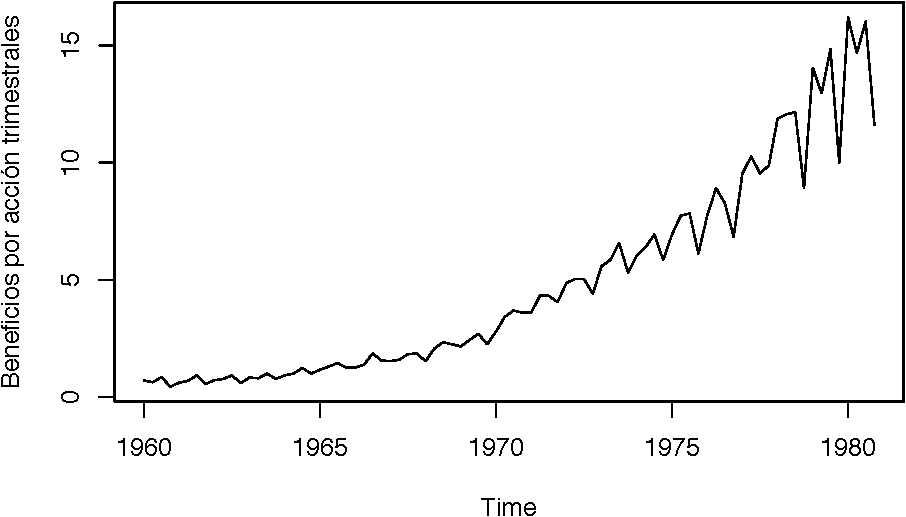
\includegraphics{Serie-de-Tiempo-en-R_files/figure-latex/unnamed-chunk-8-1} 

}

\caption{Beneficios por acción trimestrales para la compañía Johnson y Johnson}\label{fig:unnamed-chunk-8}
\end{figure}

\BeginKnitrBlock{example}
\protect\hypertarget{exm:reservas-internacionales}{}{\label{exm:reservas-internacionales}
}El archivo \emph{``ReservasInternacionales.xlsx''}, contiene el
registro mensual de Reservas Internacionales Venezolanas en millones de
dólares (\$), iniciando en el mes de enero de 1996 hasta el mes de
diciembre de 2017
\EndKnitrBlock{example}

\begin{Shaded}
\begin{Highlighting}[]
\KeywordTok{library}\NormalTok{(readxl)}
\NormalTok{reservas <-}\StringTok{ }\KeywordTok{read_excel}\NormalTok{(}\StringTok{"data/ReservasInternacionales.xlsx"}\NormalTok{)}
\NormalTok{reservas=}\KeywordTok{ts}\NormalTok{(reservas,}\DataTypeTok{start =} \DecValTok{1996}\NormalTok{,}\DataTypeTok{frequency =} \DecValTok{12}\NormalTok{)}
\KeywordTok{plot.ts}\NormalTok{(reservas[,}\DecValTok{2}\NormalTok{], }\DataTypeTok{xlab=}\StringTok{"Año"}\NormalTok{,}\DataTypeTok{ylab=}\StringTok{"Monto"}\NormalTok{,}
        \DataTypeTok{main=}\StringTok{"Reservas Internacionales de Venezuela (millones $)"}\NormalTok{)}
\end{Highlighting}
\end{Shaded}

\textbackslash{}begin\{figure\}

\{\centering 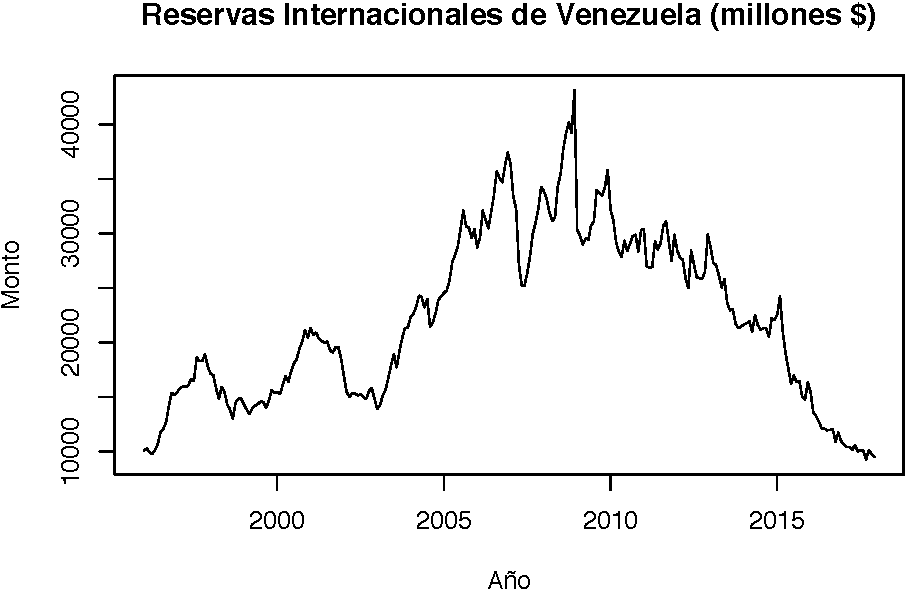
\includegraphics{Serie-de-Tiempo-en-R_files/figure-latex/unnamed-chunk-9-1}

\}

\textbackslash{}caption\{Reservas Internacionales de Venezuela (millones
\$) 1996-2017\}\label{fig:unnamed-chunk-9} \textbackslash{}end\{figure\}

\BeginKnitrBlock{example}
\protect\hypertarget{exm:precio-petroleo}{}{\label{exm:precio-petroleo} }El
archivo \emph{``PreciosPetroleoVzla.xlsx''} contiene el precio promedio
mensual de venta para el petróleo venezolano (en dólares) desde enero
2006 hasta noviembre 2017
\EndKnitrBlock{example}

\begin{Shaded}
\begin{Highlighting}[]
\KeywordTok{library}\NormalTok{(readxl)}
\NormalTok{petroleo <-}\StringTok{ }\KeywordTok{read_excel}\NormalTok{(}\StringTok{"data/PreciosPetroleoVzla.xlsx"}\NormalTok{)}
\NormalTok{petroleo=}\KeywordTok{ts}\NormalTok{(petroleo,}\DataTypeTok{start =} \DecValTok{2006}\NormalTok{,}\DataTypeTok{frequency =} \DecValTok{12}\NormalTok{)}
\KeywordTok{plot.ts}\NormalTok{(petroleo[,}\DecValTok{2}\NormalTok{], }\DataTypeTok{xlab=}\StringTok{"Año"}\NormalTok{,}\DataTypeTok{ylab=}\StringTok{"Monto"}\NormalTok{,}
        \DataTypeTok{main=}\StringTok{"Precio promedio del petróleo venezolano (en dolares $)"}\NormalTok{)}
\end{Highlighting}
\end{Shaded}

\textbackslash{}begin\{figure\}

\{\centering 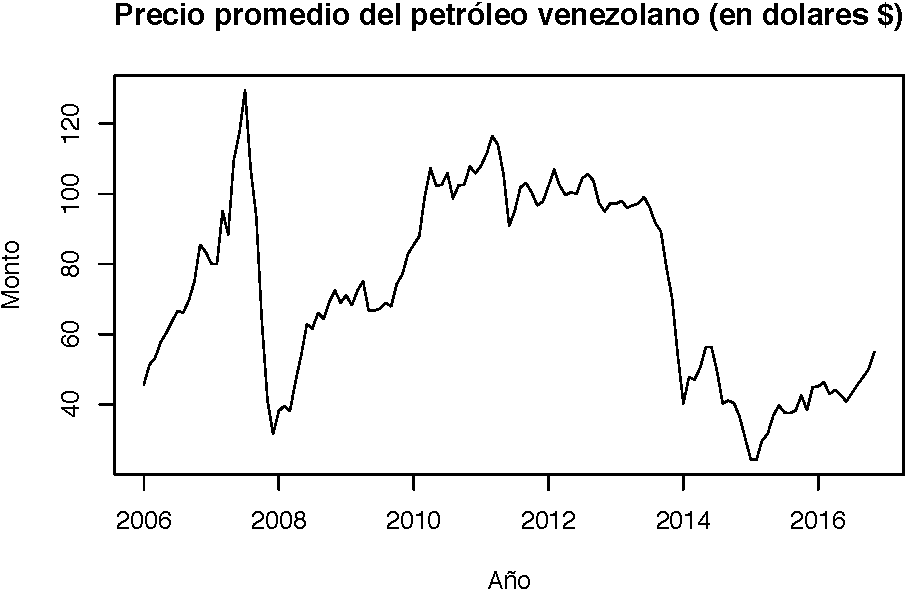
\includegraphics{Serie-de-Tiempo-en-R_files/figure-latex/unnamed-chunk-10-1}

\}

\textbackslash{}caption\{Precio promedio del petróleo venezolano (en
dolares \$) 2006-2017\}\label{fig:unnamed-chunk-10}
\textbackslash{}end\{figure\}

\BeginKnitrBlock{example}
\protect\hypertarget{exm:indice-dow-jones}{}{\label{exm:indice-dow-jones}
}El archivo \emph{``IndiceDowJones.xlsx''} contiene los valores
histórico del Índice Dow-Jones desde enero de 1930 hasta octubre de
2017. En el archivo podems notar que desde enero de 1930 hasta diciembre
de 1994, los registros son el promedio semanal, a partir de enero de
1995, los registros son diarios. La primera columa es la fecha, la
segunda columna es el valor de apertura, la tercera columna el valor
máximo, la cuarta el valor mínimo, la quinta el último valor del índice
o valor de cierre y la sexta columna es el volumen de acciones.
\EndKnitrBlock{example}

\begin{Shaded}
\begin{Highlighting}[]
\NormalTok{DJ=}\KeywordTok{read_excel}\NormalTok{(}\StringTok{"data/IndiceDowJones.xlsx"}\NormalTok{)}
\NormalTok{DJ=}\KeywordTok{ts}\NormalTok{(DJ)}
\KeywordTok{plot.ts}\NormalTok{(DJ[,}\OperatorTok{-}\DecValTok{1}\NormalTok{], }\DataTypeTok{xlab=}\StringTok{"Días"}\NormalTok{, }
        \DataTypeTok{main=}\StringTok{"Índice Dow-Jones desde enero 1930 hasta octubre 2017"}\NormalTok{)}
\end{Highlighting}
\end{Shaded}

\begin{figure}

{\centering 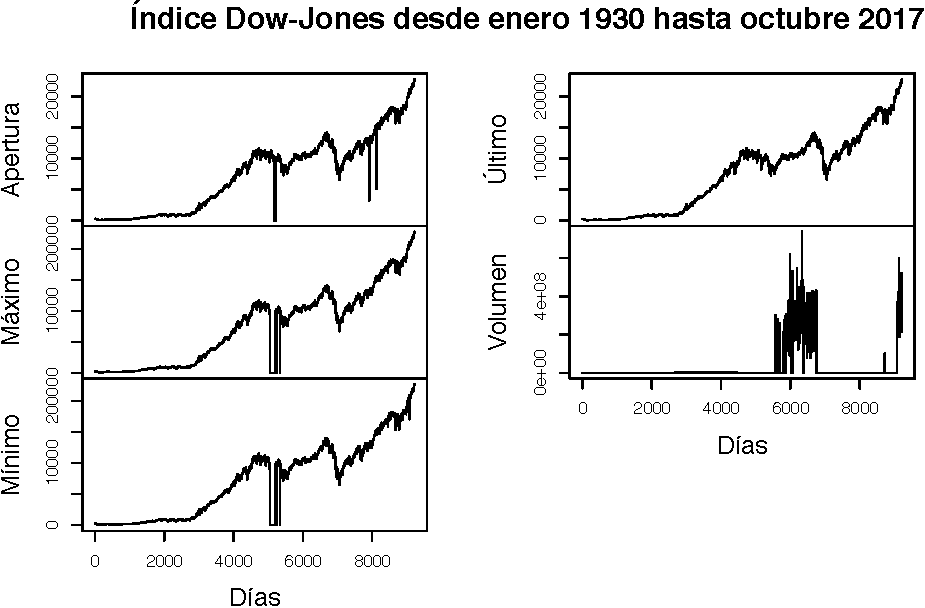
\includegraphics{Serie-de-Tiempo-en-R_files/figure-latex/unnamed-chunk-11-1} 

}

\caption{Índice Dow-Jones desde enero 1930 hasta octubre 2017}\label{fig:unnamed-chunk-11}
\end{figure}

\BeginKnitrBlock{example}
\protect\hypertarget{exm:Bolsa-Valores-New-York}{}{\label{exm:Bolsa-Valores-New-York}
}La figura siguiente muestra los porcentajes de cambio diario de la
Bolsa de Valores de New York desde el 2 de febrero de 1984 hasta el 31
de diciembre de 1991. Como se ve hay una caída fuerte, esta ocurrió el
19 de octubre de 1987 en \(t=938\). El archivo de datos es
\emph{``nyse.txt''}.
\EndKnitrBlock{example}

\begin{Shaded}
\begin{Highlighting}[]
\NormalTok{NYSE=}\KeywordTok{ts}\NormalTok{(}\KeywordTok{scan}\NormalTok{(}\StringTok{"data/nyse.txt"}\NormalTok{))}
\KeywordTok{plot}\NormalTok{(NYSE,}\DataTypeTok{xlab=}\StringTok{"Tiempo"}\NormalTok{,}\DataTypeTok{ylab=}\StringTok{"Porcentaje de cambio, NYSE"}\NormalTok{)}
\end{Highlighting}
\end{Shaded}

\begin{figure}

{\centering 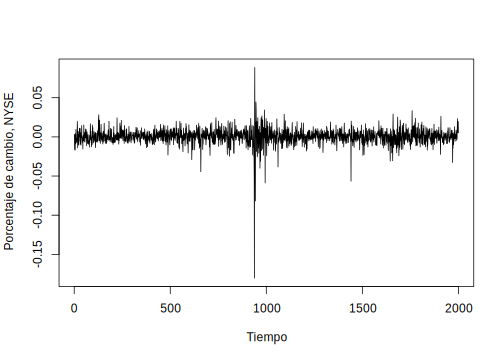
\includegraphics{Serie-de-Tiempo-en-R_files/figure-latex/unnamed-chunk-12-1} 

}

\caption{Porcentaje de cambio de la bolsa de New York}\label{fig:unnamed-chunk-12}
\end{figure}

\BeginKnitrBlock{example}
\protect\hypertarget{exm:euribor}{}{\label{exm:euribor} }La evolución del
EURIBOR es algo que fluctúa a diario. Se entiende por EURIBOR (Euro
Interbank Offered Rate) el tipo de interés, promovido por el Instituto
Europeo de Mercados Monetarios (EMMI), consistente en la media
aritmética simple de los valores diarios con días de mercado para
operaciones de depósitos en euros a plazo de uno/tres/seis/doce meses y
referido al día quince del mes anterior al comienzo de cada período de
interés o al día siguiente hábil si aquel no lo fuese, calculado a
partir del ofertado por una muestra de Bancos para operaciones entre
entidades de similar calificación.

A continuación mostramos dos series del EURIBOR. La primera es la
evolución histórica anual del EURIBOR desde su implantación en 1999
hasta 2018, los datos se corresponden al mes de enero de cada año. La
segunda es la evolución mensual desde enero de 2007 hasta marzo de 2018.
\EndKnitrBlock{example}

\begin{Shaded}
\begin{Highlighting}[]
\NormalTok{EURIBORa<-}\KeywordTok{read_excel}\NormalTok{(}\StringTok{"data/EURIBOR-anual.xlsx"}\NormalTok{)}
\KeywordTok{plot}\NormalTok{(EURIBORa,}\DataTypeTok{type=}\StringTok{"l"}\NormalTok{, }\DataTypeTok{col =} \StringTok{"blue"}\NormalTok{, }\DataTypeTok{xlab =} \StringTok{"Periodo"}\NormalTok{, }
     \DataTypeTok{main=}\StringTok{"Serie EURIBOR anual (1999-2018)"}\NormalTok{)}
\KeywordTok{grid}\NormalTok{(}\DataTypeTok{col =} \StringTok{"gray"}\NormalTok{)}
\end{Highlighting}
\end{Shaded}

\begin{figure}

{\centering 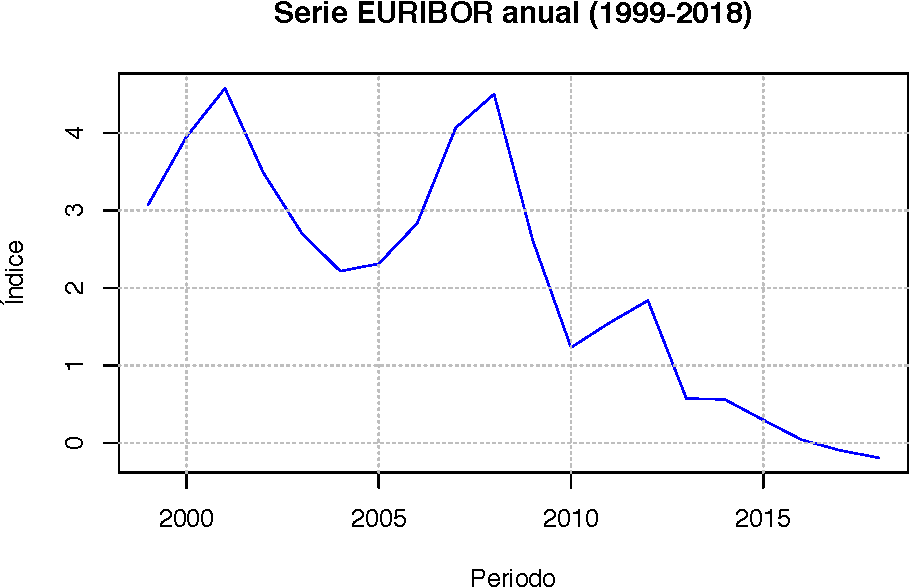
\includegraphics{Serie-de-Tiempo-en-R_files/figure-latex/unnamed-chunk-13-1} 

}

\caption{Evolución anual del EURIBOR (1999-2018)}\label{fig:unnamed-chunk-13}
\end{figure}

\begin{Shaded}
\begin{Highlighting}[]
\NormalTok{EURIBORm<-}\KeywordTok{read_excel}\NormalTok{(}\StringTok{"data/EURIBOR-mensual.xlsx"}\NormalTok{)}
\NormalTok{EURIts<-}\KeywordTok{ts}\NormalTok{(EURIBORm[,}\DecValTok{2}\NormalTok{],}\DataTypeTok{start =} \DecValTok{2007}\NormalTok{, }\DataTypeTok{frequency =} \DecValTok{12}\NormalTok{)}
\KeywordTok{plot.ts}\NormalTok{(EURIts,}\DataTypeTok{xlab =} \StringTok{"Periodo"}\NormalTok{, }\DataTypeTok{col =} \StringTok{"blue"}\NormalTok{, }
        \DataTypeTok{main=}\StringTok{"Serie EURIBOR mensual (enero 2007- marzo 2018)"}\NormalTok{)}
\KeywordTok{grid}\NormalTok{(}\DataTypeTok{col =} \StringTok{"gray"}\NormalTok{)}
\end{Highlighting}
\end{Shaded}

\begin{figure}

{\centering 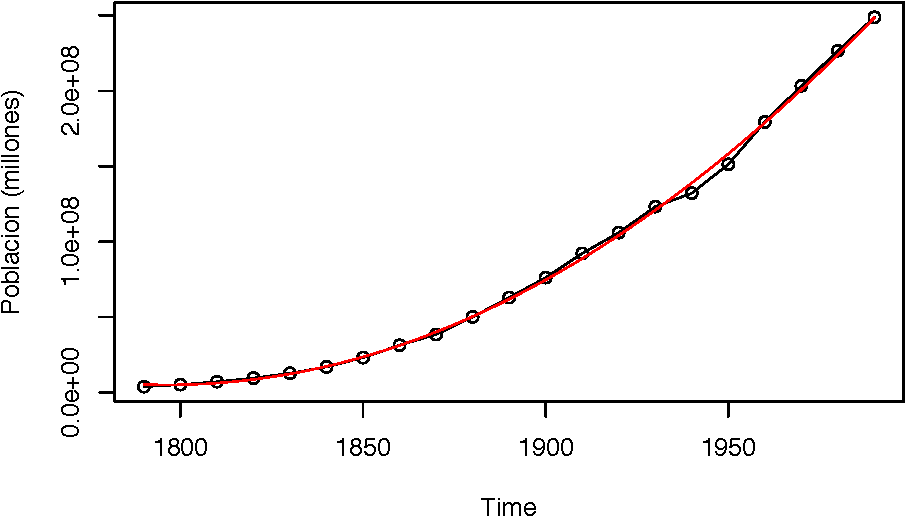
\includegraphics{Serie-de-Tiempo-en-R_files/figure-latex/unnamed-chunk-14-1} 

}

\caption{Evolución mensual del EURIBOR (2007-2018)}\label{fig:unnamed-chunk-14}
\end{figure}

\BeginKnitrBlock{example}
\protect\hypertarget{exm:cambio-dolar-euro}{}{\label{exm:cambio-dolar-euro}
}El archivo \emph{Cambio-EUR-USD.xlsx} contiene el histórico de la
cotización dolar estadounidense versus el euro desde el 01/05/2017 hasta
el 26/04/2018. En la primera columna se muestra la fecha, la segunda
columna el precio de apertura, la tercera el precio de cierre, la cuarta
la diferencia en \%, la quinta el precio máximo del día, la sexta el
precio mínimo y la utlima el volumen de transacciones. A continuación
presentamos los gráficos de apertura, cierre, máximo y mínimo.
\EndKnitrBlock{example}

\begin{Shaded}
\begin{Highlighting}[]
\NormalTok{Cambio<-}\KeywordTok{read_excel}\NormalTok{(}\StringTok{"data/Cambio-EUR-USD.xlsx"}\NormalTok{)}
\KeywordTok{par}\NormalTok{(}\DataTypeTok{mfrow=}\KeywordTok{c}\NormalTok{(}\DecValTok{3}\NormalTok{,}\DecValTok{2}\NormalTok{))}
\KeywordTok{plot}\NormalTok{(Cambio}\OperatorTok{$}\NormalTok{Fecha,Cambio}\OperatorTok{$}\NormalTok{Apertura, }\DataTypeTok{col=}\StringTok{"blue"}\NormalTok{, }\DataTypeTok{type =} \StringTok{"l"}\NormalTok{,}
     \DataTypeTok{xlab =} \StringTok{"Periodo"}\NormalTok{, }\DataTypeTok{ylab =} \StringTok{"Cotizacion"}\NormalTok{,}
     \DataTypeTok{main =} \StringTok{"Apertura"}\NormalTok{)}
\KeywordTok{plot}\NormalTok{(Cambio}\OperatorTok{$}\NormalTok{Fecha,Cambio}\OperatorTok{$}\NormalTok{Cierre, }\DataTypeTok{col=}\StringTok{"blue"}\NormalTok{, }\DataTypeTok{type =} \StringTok{"l"}\NormalTok{,}
     \DataTypeTok{xlab =} \StringTok{"Periodo"}\NormalTok{, }\DataTypeTok{ylab =} \StringTok{"Cotizacion"}\NormalTok{,}
     \DataTypeTok{main =} \StringTok{"Cierre"}\NormalTok{)}
\KeywordTok{plot}\NormalTok{(Cambio}\OperatorTok{$}\NormalTok{Fecha,Cambio}\OperatorTok{$}\NormalTok{Máximo, }\DataTypeTok{col=}\StringTok{"blue"}\NormalTok{, }\DataTypeTok{type =} \StringTok{"l"}\NormalTok{,}
     \DataTypeTok{xlab =} \StringTok{"Periodo"}\NormalTok{, }\DataTypeTok{ylab =} \StringTok{"Cotizacion"}\NormalTok{,}
     \DataTypeTok{main =} \StringTok{"Máximo"}\NormalTok{)}
\KeywordTok{plot}\NormalTok{(Cambio}\OperatorTok{$}\NormalTok{Fecha,Cambio}\OperatorTok{$}\NormalTok{Mínimo, }\DataTypeTok{col=}\StringTok{"blue"}\NormalTok{, }\DataTypeTok{type =} \StringTok{"l"}\NormalTok{,}
     \DataTypeTok{xlab =} \StringTok{"Periodo"}\NormalTok{, }\DataTypeTok{ylab =} \StringTok{"Cotizacion"}\NormalTok{,}
     \DataTypeTok{main =} \StringTok{"Mínimo"}\NormalTok{)}
\KeywordTok{plot}\NormalTok{(Cambio}\OperatorTok{$}\NormalTok{Fecha,Cambio}\OperatorTok{$}\StringTok{`}\DataTypeTok{Dif.%}\StringTok{`}\NormalTok{, }\DataTypeTok{col=}\StringTok{"blue"}\NormalTok{, }\DataTypeTok{type =} \StringTok{"l"}\NormalTok{,}
     \DataTypeTok{xlab =} \StringTok{"Periodo"}\NormalTok{, }\DataTypeTok{ylab =} \StringTok{"Porcentaje"}\NormalTok{,}
     \DataTypeTok{main =} \StringTok{"Diferencia (apetura-cierre) %"}\NormalTok{)}
\KeywordTok{plot}\NormalTok{(Cambio}\OperatorTok{$}\NormalTok{Fecha,Cambio}\OperatorTok{$}\NormalTok{Volumen, }\DataTypeTok{col=}\StringTok{"blue"}\NormalTok{, }\DataTypeTok{type =} \StringTok{"l"}\NormalTok{,}
     \DataTypeTok{xlab =} \StringTok{"Periodo"}\NormalTok{, }\DataTypeTok{ylab =} \StringTok{"Monto"}\NormalTok{,}
     \DataTypeTok{main =} \StringTok{"Volumen"}\NormalTok{)}
\end{Highlighting}
\end{Shaded}

\begin{figure}

{\centering 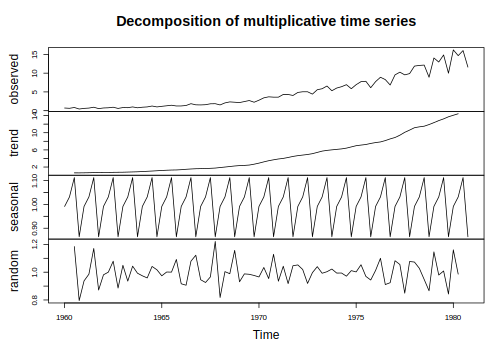
\includegraphics{Serie-de-Tiempo-en-R_files/figure-latex/unnamed-chunk-15-1} 

}

\caption{Histórico de cambio del USD vs. EUR (01/05/2017 al 26/04/2018)}\label{fig:unnamed-chunk-15}
\end{figure}

\subsection{Clasificación de las series de
tiempo}\label{clasificacion-de-las-series-de-tiempo}

Como se ha mostrado en los ejemplos anteriores, hay una amplia variedad
de series de tiempo que pueden clasificarse en varias categorías desde
varios puntos de vista.

\begin{itemize}
\item
  \textbf{Series de tiempo continuas y discretas}. Los datos registrados
  continuamente, por ejemplo, por un dispositivo analógico, se denominan
  series de tiempo continuas. Por otra parte, los datos observados en
  ciertos intervalos de tiempo, como la presión atmosférica medida cada
  hora, se denominan series de tiempo discretas. Existen dos tipos de
  series de tiempo discretas: una en la que las observaciones de los
  datos se realizan a intervalos de igual espaciamiento y otra en la que
  las observaciones de los datos se realizan a intervalos de
  espaciamiento desigual. Aunque las series de tiempo mostradas en los
  ejemplos anteriores están conectadas continuamente por líneas sólidas,
  todas ellas son series de tiempo discretas. A partir de ahora en este
  libro, consideramos sólo series de tiempo discretas registradas a
  intervalos igualmente espaciados, porque las series de tiempo que
  analizamos en ordenadores digitales son generalmente series de tiempo
  discretas.
\item
  \textbf{Series de tiempo univariadas y multivariadas}. Las series de
  tiempo que consisten en una sola observación en cada punto temporal,
  como se muestran en los ejemplos 1.1, 1.2, 1.3 y 1.5, se denominan
  series de tiempo univariadas. Por otra parte, las series de tiempo que
  se obtienen grabando simultáneamente dos o más fenómenos como los
  ilustrados en el ejemplo 1.4 se denominan series de tiempo
  multivariadas. Sin embargo, puede ser difícil distinguir entre series
  de tiempo univariadas y multivariadas desde su naturaleza; más bien,
  la distinción se hace desde el punto de vista del analista y por
  varios otros factores, como la restricción de la medición y los
  conocimientos empíricos o teóricos sobre el tema. Desde el punto de
  vista del modelado estadístico, la selección de variables en sí misma
  es un problema importante en el análisis de series de tiempo.
\item
  \textbf{Series de tiempo estacionarias y no estacionarias}. Una serie
  de tiempo es un registro de un fenómeno que varía irregularmente con
  el tiempo. En el análisis de series de tiempo, las series de tiempo de
  variación irregular se expresan generalmente mediante modelos
  estocásticos. En algunos casos, un fenómeno aleatorio puede ser
  considerado como la realización de un modelo estocástico con una
  estructura de variación temporal. Estas series de tiempo se denominan
  series de tiempo estacinarias. El ejemplo 1.5 es un ejemplo típico de
  una serie de tiempo estacionaria. Por otra parte, si la estructura
  estoc?stica de una serie de tiempo cambia con el tiempo, se denomina
  serie de tiempo no estacionaria. Como ejemplos típicos de series de
  tiempo no estacionarias, considere la serie en los ejemplos 1.1 a 1.4
  . Se puede observar que los valores medios cambian a lo largo del
  tiempo.
\item
  \textbf{Series de tiempo gaussianas y no gaussianas}. Cuando una
  distribución de una serie de tiempo sigue una distribución normal, la
  serie de tiempo se denomina serie de tiempo gaussiana; de lo
  contrario, se denomina serie de tiempo no gausiana. La mayoría de los
  modelos considerados en este libro son modelos gaussianos, asumiendo
  que las series de tiempo siguen distribuciones gaussianas. Al igual
  que en el caso del ejemplo 1.3, el patrón de las series de tiempo es a
  veces asimétrico, de modo que la distribución marginal no puede
  considerarse gaussiana. Incluso en tal situación, podemos obtener una
  serie de tiempo gaussiana aproximada mediante una transformación de
  datos apropiada.
\item
  \textbf{Series de tiempo lineales y no lineales}. Una serie de tiempo
  expresable como la salida de un modelo lineal se denomina serie de
  tiempo lineal. Por el contrario, la salida de un modelo no lineal se
  denomina serie de tiempo no lineal.
\item
  \textbf{Datos faltantes y valores atípicos}. En el modelado de series
  de tiempo de problemas del mundo real, a veces necesitamos tratar con
  observaciones faltante y valores atípicos. Algunos valores de las
  series de tiempo que no se han registrado por algunas razones se
  denominan observaciones que faltan en las series de tiempo. Los
  valores atípicos (observaciones exteriores) pueden ocurrir debido al
  comportamiento extraordinario del objeto, mal funcionamiento del
  dispositivo de observación o errores en el registro. En los datos de
  los ejemplos 1.4 y 1.5 se pueden observar datos atípicos. En el
  ejemplo 1.4 podemos notar caídas en los índices del DowJones y en el
  ejemplo 1.4 podemos notar una fuerte caída en el porcentaje de cambio
  de diario ocurrido el 19 de octubre de 1987.
\end{itemize}

\section{Componentes de una serie de
tiempo}\label{componentes-de-una-serie-de-tiempo}

El análisis clásico de las series de tiempo se basa en la suposición de
que los valores que toma la variable de observación es la consecuencia
de tres componentes, cuya actuación conjunta da como resultado los
valores medidos, estos componentes son:

\begin{enumerate}
\def\labelenumi{\arabic{enumi})}
\item
  \textbf{Componente de tendencia}. Se puede definir como un cambio a
  largo plazo que se produce en la relación al nivel medio, o el cambio
  a largo plazo de la media. La tendencia se identifica con un
  movimiento suave de la serie a largo plazo.
\item
  \textbf{Componente estacional}. Muchas series de tiempo presentan
  cierta periodicidad o dicho de otro modo, variación de cierto período
  (semestral, mensual, etc.). Por ejemplo las Ventas al Detalle en
  Puerto Rico aumentan por los meses de noviembre y diciembre por las
  festividades navideñas. Estos efectos son fáciles de entender y se
  pueden medir explícitamente o incluso se pueden eliminar de la serie
  de datos, a este proceso se le llama desestacionalización de la serie.
\item
  \textbf{Componente aleatoria}. Esta componente no responde a ningún
  patrón de comportamiento, sino que es el resultado de factores
  fortuitos o aleatorios que inciden de forma aislada en una serie de
  tiempo.
\end{enumerate}

De los tres componentes anteriores los dos primeros son componentes
determinísticos, mientras que la última es aleatoria.

Los modelos que se utilizan con más frecuencia son:

\begin{itemize}
\item
  \textbf{Modelo aditivo}: \(X_t=T_t+E_t+\epsilon_t\)
\item
  \textbf{Modelos multiplicativos}:

  \begin{itemize}
  \item
    \emph{Puro}: \(X_t = T_t\times E_t\times\epsilon_t\)
  \item
    \emph{Mixto}: \(X_t = T_t\times E_t+\epsilon_t\)
  \end{itemize}
\end{itemize}

La elección de uno de estos modelos se hará de manera que el modelo
seleccionado sea capaz de agrupar las principales características
observadas en el gráfico de la serie en estudio.

\subsection{El Modelo Aditivo de Componentes de Series de
Tiempo}\label{el-modelo-aditivo-de-componentes-de-series-de-tiempo}

Dada una serie \(X_t, t=1,\ldots,n\), el \emph{Modelo Aditivo de
Componentes} consiste en asumir que \(X_t\) se puede descomponer en tres
componentes:

\begin{equation}
X_t = T_t+E_t+\epsilon_t
\label{eq:eq-modelo-aditivo}
\end{equation}

donde \(T_t\) es la componente de tendencia, \(E_t\) es la componente
estacional y \(\epsilon_t\) es la componente aleatoria o de errores. Las
componentes \(T_t\) y \(E_t\) son funciones de \(t\) determinísticas. Su
evolución es perfectamente predecible.

Este modelo es apropiado cuando la magnitud de la fluctuaciones
estacionales de la serie no varía al hacerlo la tendencia.

La componente \(T_t\) en algunos casos también puede ser una componente
estacional, pero de baja frecuencia, o, equivalentemente, una componente
con período muy grande. Por ejemplo, en una serie diaria, \(E_t\) puede
tener período 30 días, y \(T_t\) período 360 días.

En la Figura \ref{grafica-tema3-modelo-aditivo} se muestra la idea de la
descomposición. Al superponer las series en los gráficos (a), (b) y (c)
se obtiene la serie en el gráfico (d).

\begin{figure}

{\centering 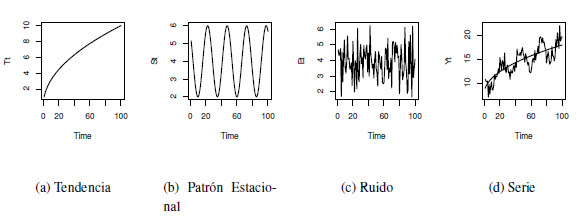
\includegraphics[width=8.12in]{images/Grafica-tema3-modelo-aditivo} 

}

\caption{Modelo aditivo de series de tiempo}\label{fig:unnamed-chunk-16}
\end{figure}

Asumiendo el modelo aditivo, el análisis de series de tiempo consiste en
modelar y estimar \(T_t\) y \(E_t\) y luego extraerlas de \(X_t\) para
obtener \(\hat{\epsilon}_t = X_t - \hat{T}_t - \hat{E}_t\). La serie
\(\hat{\epsilon}_t\) se modela y estima para finalmente reconstruir
\(X_t\), \(\hat{X}_t = \hat{T}_t+\hat{E}_t+\hat{\epsilon}_t\), y poder
realizar el pronóstico
\(\hat{X}_{t+h}=\hat{T}_{t+h}+\hat{E}_{t+h}+\hat{\epsilon}_{t+h}\),
utilizando la información disponible \(X_t,\ldots,X_n\) con
\(h=1,2,\ldots,m\). Sin embargo, puede suceder que la serie
\(\hat{\epsilon}_t\) sea incorrelacionada, es decir,
\(Corr(\hat{\epsilon}_t,\hat{\epsilon}_{t+s}) = 0\), para \(s\neq0\). En
este caso \(\hat{\epsilon}_{t+h}=0\) para todo \(h>0\).

En \textbf{R} podemos descomponer una serie de tiempo usando la función
\emph{stl()} o la función \emph{decompose()}. Retomando la serie de
beneficios trimestrales de las acciones de Johnson y Johnson (Ejemplo
\ref{exm:ejem-beneficios-acciones}) podemos observar la descomposición
de la misma. En la parte superior de la gráfica se observa la serie
original, en el gráfico siguiente la estacionalidad, en el tercero la
tendencia y en el gráfico inferior los residuales.

\begin{Shaded}
\begin{Highlighting}[]
\KeywordTok{plot}\NormalTok{(}\KeywordTok{decompose}\NormalTok{(jj, }\DataTypeTok{type =} \StringTok{"additive"}\NormalTok{, }\DataTypeTok{filter =} \OtherTok{NULL}\NormalTok{))}
\end{Highlighting}
\end{Shaded}

\begin{figure}

{\centering 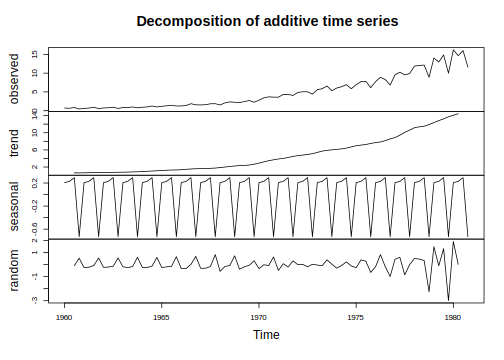
\includegraphics{Serie-de-Tiempo-en-R_files/figure-latex/unnamed-chunk-17-1} 

}

\caption{Descomposición aditiva de la serie Johnson y Johnson}\label{fig:unnamed-chunk-17}
\end{figure}

La función \emph{stl()} es más sofisticada que \emph{decompose()}, la
misma usa la descomposición de estacionalidad y tendencia de Loess
(Seasonal and Trend decomposition using Loess) el cual es un método
robusto y versátil para la descomposición de series de tiempo. El método
STL fue desarrollado por Cleveland et al. (1990). A continuación
mostramos la misma serie de beneficios de acciones de Johnson y Johnson
usando esta función.

\begin{Shaded}
\begin{Highlighting}[]
\KeywordTok{plot}\NormalTok{(}\KeywordTok{stl}\NormalTok{(jj,}\DataTypeTok{s.window=}\StringTok{"periodic"}\NormalTok{), }\DataTypeTok{col=}\StringTok{"blue"}\NormalTok{,}
     \DataTypeTok{main=}\StringTok{"Descomposicion de la serie Johnson y Johnson"}\NormalTok{)}
\end{Highlighting}
\end{Shaded}

\begin{figure}

{\centering 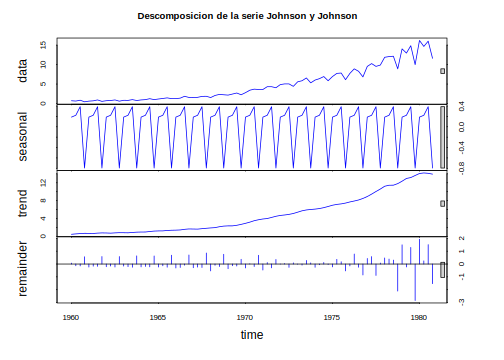
\includegraphics{Serie-de-Tiempo-en-R_files/figure-latex/unnamed-chunk-18-1} 

}

\caption{Descomposición de la serie Johnson y Johnson usando la descomposición de Loess (STL)}\label{fig:unnamed-chunk-18}
\end{figure}

\subsection{El Modelo Multiplicativo de Componentes de Series de
Tiempo}\label{el-modelo-multiplicativo-de-componentes-de-series-de-tiempo}

Dada una serie de tiempo \(X_t,t=1,\ldots,n\), el \emph{Modelo
Multiplicativo de Componentes} consiste en asumir que \(X_t\) se puede
descomponer de una de las siguientes maneras:

\begin{itemize}
\tightlist
\item
  \emph{Puro}:

  \begin{equation}
  X_t = T_t\times E_t\times\epsilon_t
  \label{eq:eq-modelo-multiplicativo-puro}
  \end{equation}
\item
  \emph{Mixto}:

  \begin{equation}
  X_t = T_t\times E_t+\epsilon_t
  \label{eq:eq-modelo-multiplicativo-mixto}
  \end{equation}
\end{itemize}

donde \(T_t\) es la componente de tendencia, \(E_t\) es la componente
estacional y \(\epsilon_t\) es la componente aleatoria o de errores.
Estos modelos son apropiados cuando la magnitud de las fluctuaciones
estacionales de la serie crece y decrece proporcionalmente con los
crecimientos y decrecimientos de la tendencia respectivamente.

Usamos la misma función \emph{decompose()} para realizar la
descomposición multiplicativa de la serie de tiempo, para ello en `type'
cambiamos ``additive'' por ``multiplicative''

\begin{Shaded}
\begin{Highlighting}[]
\KeywordTok{plot}\NormalTok{(}\KeywordTok{decompose}\NormalTok{(jj, }\DataTypeTok{type =} \StringTok{"multiplicative"}\NormalTok{, }\DataTypeTok{filter =} \OtherTok{NULL}\NormalTok{))}
\end{Highlighting}
\end{Shaded}

\begin{figure}

{\centering 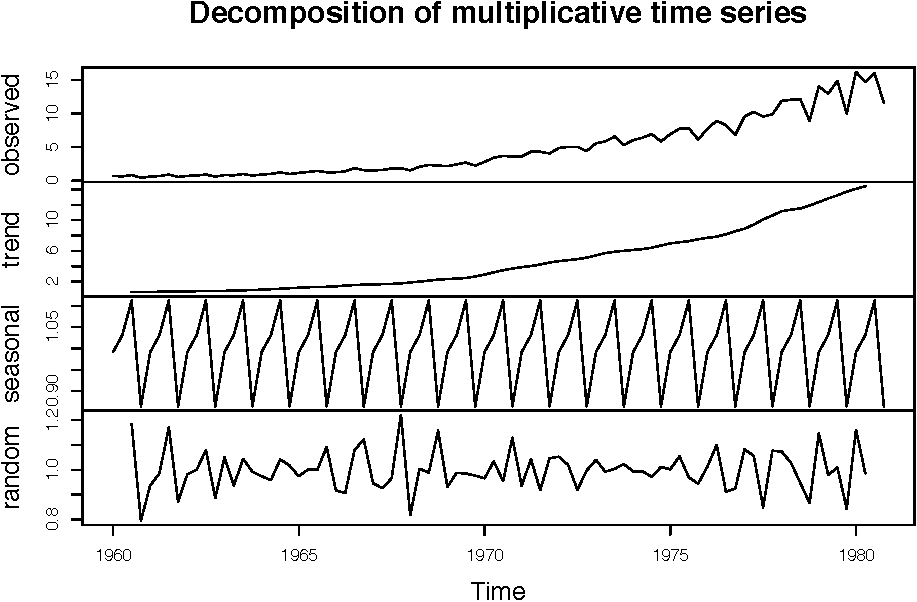
\includegraphics{Serie-de-Tiempo-en-R_files/figure-latex/unnamed-chunk-19-1} 

}

\caption{Descomposición multiplicativa de la serie Johnson y Johnson}\label{fig:unnamed-chunk-19}
\end{figure}

\chapter{Características de series de
tiempo}\label{caracteristicas-de-series-de-tiempo}

El objetivo primario en el análisis de Series de Tiempo es desarrollar
modelos matemáticos que provean una descripción apropiada para los datos
muestrales, como los vistos en los ejemplos del capítulo anterior. Así,
lo primero que hacemos es utilizar la definición
\ref{def:defi-serie-tiempo}, para tener un soporte estadístico. En este
capítulo daremos algunas definiciones que serán de uso general en todo
el resto del libro, también sedescribiran algunos métodos para el
análisis exploratorio de las series de tiempo

\section{Medidas de dependencia para series de
tiempo}\label{medidas-de-dependencia-para-series-de-tiempo}

\BeginKnitrBlock{definition}
\protect\hypertarget{def:defi-proceso-estocastico}{}{\label{def:defi-proceso-estocastico}
}Un \textbf{proceso estocástico} es una familia de variables aleatorias
indexadas \(x(\omega,t)\) ó \(x_t(\omega)\) donde \(t\) pertenece a un
conjunto de índices \(T\) y \(\omega\) pertenece a un espacio muestral
\(\Omega\). Si \(t=t^*\) fijo, \(x(\omega,t^*)\) es una variable
aleatoria. Si \(\omega=\omega^*\) fijo, \(x(\omega^*,t)\) es una función
de \(t\), y se llama una realización del proceso. Una \textbf{serie de
tiempo} es la realización de un proceso estocástico.
\EndKnitrBlock{definition}

Una descripción completa de una serie de tiempo, observada como una
colección de \(n\) variables aleatorias en puntos de tiempo enteros
arbitrarios \(t_1,t_2,\ldots,t_n\), para cada entero positivo \(n\), es
proporcionada por la función de distribución conjunta, evaluada como la
probabilidad de que los valores de la serie sean conjuntamente menor que
\(n\) constantes \(c_1,c_2,\ldots,c_n\), esto es

\begin{equation}
F(c_1,c_2,\ldots,c_n)=P(x_{t_1}\leq c_1,x_{t_2}\leq c_2,\ldots,x_{t_n}\leq c_n).
\label{eq:eq-distribucion-conjunta}
\end{equation}

Desafortunadamente, la función de distribución multidimensional
usualmente no se puede escribir fácilmente a menos que las variables
aleatorias tengan distribución normal conjunta, en cuyo caso, la
ecuación \eqref{eq:eq-distribucion-conjunta} llega a ser la distribución
normal multivariada usual.

Un caso particular en la cual la función de distribución
multidimensional es fácil de escribir, será en el caso de variables
aleatorias normal estándar independientes e idénticamente distribuidas,
para lo cual la función de distribución se puede expresar como el
producto de las distribuciones marginales, es decir,

\begin{equation}
F(c_1,c_2,\ldots,c_n)=\prod_{t_1}^{n}\Phi(c_t)
\label{eq:eq-distribucion-producto-marginal}
\end{equation}

donde

\begin{equation}
\Phi(x)=\frac{1}{\sqrt{2\pi}}\int_{-\infty}^{x}\mathbb{E}xp\left\{-\frac{z^2}{2}\right\}dz\label{eq:eq-distribucion-normal}
\end{equation}

es la función de distribución normal estándar acumulada.

Aunque la función de distribución multidimensional describa los datos
completamente, esto es un instrumento poco manejable para mostrar y
analizar datos de series de tiempo. La función de distribución
\eqref{eq:eq-distribucion-conjunta} debe ser evaluada como una función de
\(n\) argumentos, entonces cualquier graficación de las correspondientes
funciones de densidad multivariante es prácticamente imposible. La
función de distribución unidimensional

\[F_t(x)=P\{x_t\leq x\}\] o la correspondiente función de densidad
unidimensional

\[f_t(x)=\frac{\partial F_t(x)}{\partial x},\] cuando existen, a menudo
son más útiles para determinar si una coordenada en particular de la
serie de tiempo tiene una función de densidad conocida, como la
distribución normal (gaussiana), por ejemplo.

\BeginKnitrBlock{definition}
\protect\hypertarget{def:defi-funcion-media}{}{\label{def:defi-funcion-media}
}La \textbf{función de media} es definida como

\begin{equation}
\mu_{xt}=\mathbb{E}(x_t)=\int_{-\infty}^{\infty}xf_t(x)dx,
\label{eq:eq-funcion-media}
\end{equation}

en caso de que exista, donde \(\mathbb{E}\) denota el operador usual de
esperanza. Cuando no haya confusión sobre a que serie de tiempo nos
referimos, escribiremos \(\mu_{xt}\) como \(\mu_t\).
\EndKnitrBlock{definition}

Lo importante de comprender sobre \(\mu_t\) consiste en que es una media
teórica para la serie de tiempo en un punto particular, donde la media
se asume o calcula sobre todos los posibles eventos que podrían haber
producido \(x_t\).

\BeginKnitrBlock{definition}
\protect\hypertarget{def:defi-funcion-autocovarianza}{}{\label{def:defi-funcion-autocovarianza}
}La \textbf{función de autocovarianza} es definida como producto del
segundo momento

\begin{equation}
\gamma_x(s,t)=\mathbb{E}[(x_s-\mu_s)(x_t-\mu_t)],
\label{eq:eq-funcion-autocovarianza}
\end{equation}

para todo \(t\) y \(s\). cuando no haya confusión en la existencia sobre
a que serie nos referimos, escribiremos \(\gamma_x(s,t)=\gamma(s,t)\).
\EndKnitrBlock{definition}

Note que \(\gamma_x(s,t)=\gamma_x(t,s)\) para todo los puntos \(s\) y
\(t\). La función de autocovarianza mide la dependencia lineal entre dos
puntos de la misma serie en diferentes tiempos. La autocovarianza
\eqref{eq:eq-funcion-autocovarianza} es el promedio de los productos
cruzados relacionado con la densidad conjunta \(F(x_s,x_t)\). Es claro
que, para \(s=t\), la autocovarianza se reduce a la varianza (en el caso
finito), dado que

\begin{equation}
\gamma_x(t,t)=\mathbb{E}[(x_t-\mu_t)^2]
\label{eq:eq-funcion-autocovarianza-varianza}
\end{equation}

Otro función de medida de tendencia importante es la \emph{función de
autocorrelación}.

\BeginKnitrBlock{definition}
\protect\hypertarget{def:defi-acf}{}{\label{def:defi-acf} }La
\textbf{función de autocorrelación (ACF)} (ACF, siglas en ingles:
Autocorrelation Function) se define como

\begin{equation}
\rho(s,t)=\frac{\gamma(s,t)}{\sqrt{\gamma(s,s)\gamma(t,t)}}
\label{eq:eq-funcion-autocorrelacion}
\end{equation}
\EndKnitrBlock{definition}

La \(ACF\) mide la predictibilidad lineal de una serie de tiempo en
tiempo \(t\), digamos \(x_t\) usando solo el valor \(x_s\). Es fácil de
demostrar que \(-1\leq\rho(s,t)\leq1\) usando la desigualdad de
Cauchy-Schwarz \footnote{Note que la desigualdad de Cauchy-Schwartz
  implica \(|\gamma(s,t)|^2\leq\gamma(s,s)\gamma(t,t)\).\}.}

Si podemos predecir \(x_t\) exactamente de \(x_s\) a través de la
relación lineal \(x_t=\beta_0+\beta_1x_s\) entonces la correlación será
1 cuando \(\beta_1>0\) y \(-1\) cuando \(\beta_1<0\).

\BeginKnitrBlock{definition}
\protect\hypertarget{def:defi-covarianza-cruzada}{}{\label{def:defi-covarianza-cruzada}
}La \textbf{función de covarianza cruzada} entre dos series \(x_t\) y
\(y_t\) se define como

\begin{equation}
\gamma_{xy}(s,t)=\mathbb{E}[(x_s-\mu_{xs})(y_t-\mu_{yt})]
\label{eq:eq-funcion-covarianza-cruzada}
\end{equation}
\EndKnitrBlock{definition}

\BeginKnitrBlock{definition}
\protect\hypertarget{def:defi-ccf}{}{\label{def:defi-ccf} }La
\textbf{función de correlación cruzada (CCF)} (CCF, siglas en ingles:
Cross Correlation Function) es definida como

\begin{equation}
\rho_{xy}(s,t)=\frac{\gamma_{xy}(s,t)}{\sqrt{\gamma_x(s,s)\gamma_y(t,t)}}
\label{eq:eq-funcion-correlacion-cruzada}
\end{equation}
\EndKnitrBlock{definition}

Las definiciones anteriores de funciones de media y varianza son
completamente generales. Aunque nosotros no hayamos hecho ninguna
suposición especial sobre el comportamiento de las series de tiempo,
muchos de los ejemplos precedentes han insinuado que puede existir una
especie de regularidad en el comportamiento de las mismas. Introducimos
la noción de regularidad que usa el concepto de \emph{estacionaridad},
que ya hemos introducido empíricamente en el apartado 1.2.1
``Clasificación de las series de tiempo''

Formalmente tenemos las siguientes definiciones de estacionaridad

\BeginKnitrBlock{definition}
\protect\hypertarget{def:defi-estricta-estacionaridad}{}{\label{def:defi-estricta-estacionaridad}
}Una serie de tiempo \textbf{estrictamente estacionaria} es una serie
para la cual el comportamiento probabilístico de cada sucesión de
valores

\[\{x_{t_1},x_{t_2},\ldots,x_{t_k}\}\]

es idéntico a la serie trasladada en el tiempo

\[\{x_{t_1+h},x_{t_2+h},\ldots,x_{t_k+h}\}\]

Esto es,

\begin{equation}
P[X_{t_1}\leq c_1,\ldots,x_{t_k}\leq c_k] = P[X_{t_1+h}\leq c_1,\ldots,x_{t_k+h}\leq c_k]
\label{eq:eq-estricta-estacionaridad}
\end{equation}

para todo \(k=1,2,\ldots\), todo puntos de tiempos
\(t_1,t_2,\ldots,t_k\) y números \(c_1,c_2,\ldots,c_k\) y todo salto
\(h=\pm0,\pm1,\pm2,\ldots\).
\EndKnitrBlock{definition}

Esta definición de estacionaridad es muy fuerte para la mayoría de las
aplicaciones prácticas. Por ello necesitamos una versión menos fuerte
que imponga menos condiciones sobre las distribuciones de probabilidad,
ya que si observamos bien la ecuación
\eqref{eq:eq-estricta-estacionaridad}, lo que nos dice la misma es que
todas las posibles distribuciones de probabilidad deben ser iguales, lo
que como ya indicamos en la práctica es muy difícil de compriobar aún
para conjuntos de datos sencillos. La siguiente versión de
estacionaridad solo impone condiciones sobre los dos primeros momentos
de la serie

\BeginKnitrBlock{definition}
\protect\hypertarget{def:defi-debilmente-estacionaria}{}{\label{def:defi-debilmente-estacionaria}
}Una serie de tiempo \textbf{débilmente estacionaria} \(x_t\), es un
proceso de varianza finita tal que

\begin{enumerate}
\def\labelenumi{\arabic{enumi})}
\item
  la función de media \(\mu_t\) es constante y no depende del tiempo
  \(t\),
\item
  la función de covarianza \(\gamma(t,s)\) depende solo de las
  diferencias de \(s\) y \(t\), \(|t-s|\).
\end{enumerate}

Por consiguiente, usaremos el término \textbf{estacionaridad} para
referirnos a estcionaridad débil; si un proceso es estacinario en el
sentido estricto usaremos el término \emph{estrictamente estacionario}.
\EndKnitrBlock{definition}

\BeginKnitrBlock{remark}
\iffalse{} {Nota. } \fi{}1) Si una serie de tiempo es estrictamente
estacionaria, entonces todos las funciones de distribución multivariadas
para subconjuntos de variables deben coincidir con sus contrapartes en
el conjunto trasladado, para todos los valores del parámetro \(h\). Por
ejemplo para \(k=1\) La ecuación \eqref{eq:eq-estricta-estacionaridad}
implica que

\begin{equation}
        P\{x_s\leq c\}=P\{x_t\leq c\}
\label{eq:e1p20}
\end{equation}

para cada puntos \(s\) y \(t\).

Esta declaración implica, por ejemplo, que si la probabilidad de un
valor de una serie de tiempo muestreada cada hora es negativa a la
1:00a.m, la probabilidad a la 10:00a.m. es la misma. Además, si la
función de media, \(\mu_t\) de la serie \(x_t\) existe, \eqref{eq:e1p20}
implica que \(\mu_s=\mu_t\) para todo \(s\) y \(t\), y por consiguiente
\(\mu_t\) debe ser constante.

\begin{enumerate}
\def\labelenumi{\arabic{enumi})}
\setcounter{enumi}{1}
\tightlist
\item
  Cuando \(k=2\), podemos escribir la ecuación
  \eqref{eq:eq-estricta-estacionaridad} como
\end{enumerate}

\begin{equation}
  P\{x_s\leq c_1,x_t\leq c_2\}=P\{x_{s+h}\leq c_1,x_{t+h}\leq c_2\}
\label{eq:e1p21}
\end{equation}

para cada par de puntos \(s\) y \(t\) y salto \(h\). Entonces, si la
función de varianza del proceso existe, \eqref{eq:e1p21} implica que la
función de autocovarianza de la serie \(x_t\) satisface
\(\gamma(s,t)=\gamma(s+h,t+h)\) para todos \(s\) y \(t\) y salto \(h\).

Podemos interpretar este resultado diciendo que la función de
autocovarianza del proceso depende sólo de las diferencias de tiempo
entre \(s\) y \(t\), y no del tiempo actual.
\EndKnitrBlock{remark}

Es claro de la definición \ref{def:defi-estricta-estacionaridad} de
serie estrictamente estacionaria, que una serie de tiempo estrictamente
estacionaria con varianza finita, también es una serie estacionaria. El
recíproco no es cierto a menos que impongamos condicionaes adicionales.
Un importante caso donde estacionaridad implica estricta estacionaridad
es el caso de series de tiempo gaussianas.

Ya que la función de media \(\mathbb{E}(x_t)=\mu_t\) de una serie de
tiempo estacionaria es independiente del tiempo \(t\), escribimos

\begin{equation}
\mu_t=\mu
\label{eq:e1p22}
\end{equation}

Debido a que la función de covarianza de una serie de tiempo
estacionaria, \(\gamma(s,t)\) en tiempos \(s\) y \(t\) depende sólo de
la diferencia \(|s-t|\), podemos simplificar la notación. Sea \(s=t+h\),
donde \(h\) representa el tiempo de traslación o salto, entonces

\begin{eqnarray}
\gamma(s,t)&=&\mathbb{E}[(x_{t+h}-\mu)(x_t-\mu)]\\ \nonumber
    &=&\mathbb{E}[(x_h-\mu)(x_0-\mu)]\\
    &=&\gamma(h,0) \nonumber
    \label{eq:eq-funcion-covarianza-estacionaria}
\end{eqnarray}

no depende del argumento de tiempo \(t\); asumiendo que
\(\text{Var}(x_t)=\gamma(0,0)<\infty\). De ahora en adelante, por
conveniencia, prescindiremos del segundo argumento de \(\gamma(h,0)\),
es decir, la función de covarianza se denotará \(\gamma(h)\).

\BeginKnitrBlock{definition}
\protect\hypertarget{def:defi-autocovarianza-serie-estacionaria}{}{\label{def:defi-autocovarianza-serie-estacionaria}
}La \textbf{función de autocovarianza de una serie de tiempo
estacionaria} se escribirá como

\begin{equation}
\gamma(h)=\mathbb{E}[(x_{t+h}-\mu)(x_t-\mu)]
\label{eq:eq-funcion-autocovarianza-estacionaria}
\end{equation}
\EndKnitrBlock{definition}

\BeginKnitrBlock{definition}
\protect\hypertarget{def:defi-acf-estacionaria}{}{\label{def:defi-acf-estacionaria}
}La \textbf{función de autocorrelación (ACF) de una serie de tiempo
estacionaria} será escrita, usando \eqref{eq:eq-funcion-autocorrelacion}
como

\begin{equation}
\rho(h)=\frac{\gamma(t+h,t)}{\sqrt{\gamma(t+h,t+h)\gamma(t,t)}}=\frac{\gamma(h)}{\gamma(0)}
\label{eq:eq-funcion-autocorrelacion-estacionaria}
\end{equation}
\EndKnitrBlock{definition}

La desigualdad de Cauchy-Schwartz muestra nuevamente que
\(-1\leq\rho(h)\leq1\) para todo \(h\).

** Propiedades de la función de covarianza**

\begin{enumerate}
\def\labelenumi{\arabic{enumi})}
\tightlist
\item
  Para el valor en \(h=0\), la función de autocovarianza

  \begin{equation}
  \gamma(0)=\mathbb{E}[(x_t-\mu)^2]
  \label{eq:eq-funcion-autocovarianza-h0}
  \end{equation}

  es la varianza de la serie de tiempo; note que la desigualdad de
  Cauchy-Schwartz implica que \(|\gamma(h)|\leq\gamma(0)\).
\item
  La autocovarianza de una serie estacionaria es simétrica respecto al
  origen, esto es

  \begin{equation}
  \gamma(h)=\gamma(-h)
  \label{eq:eq-simetria-funcion-autocovarianza}
  \end{equation}

  para todo \(h\). Esta propiedad se debe a que trasladar la serie por
  \(h\) significa que

  \begin{eqnarray*}
  \gamma(h)&=&\gamma(t+h-t)\\
      &=&\mathbb{E}[(x_{t+h}-\mu)(x_t-\mu)]\\
      &=&\mathbb{E}[(x_t-\mu)(x_{t+h}-\mu)]\\
      &=&\gamma(t-(t+h))\\
      &=&\gamma(-h)
  \end{eqnarray*}

  lo cual muestra como usar la notación para demostrar el resultado.
\end{enumerate}

\BeginKnitrBlock{definition}
\protect\hypertarget{def:defi-conjuntamente-estacionarias}{}{\label{def:defi-conjuntamente-estacionarias}
}Dos series de tiempo \(x_t\) y \(x_s\) se dice que son
\textbf{conjuntamente estacionarias} si cada una de ellas es
estacionaria y la función de correlación cruzada

\begin{equation}
\gamma_{xy}(h)=\mathbb{E}[(x_{t+h}-\mu_x)(y_t-\mu_y)]
\label{eq:eq-estacionaridad-conjunta}
\end{equation}

es una función sólo del salto \(h\).
\EndKnitrBlock{definition}

\BeginKnitrBlock{definition}
\protect\hypertarget{def:defi-ccf-conjuntamente-estacionarias}{}{\label{def:defi-ccf-conjuntamente-estacionarias}
}La \textbf{función de correlación cruzada (CCF)} de dos series
conjuntamente estacionarias \(x_t\) y \(y_t\) se define como

\begin{equation}
\rho_{xy}(h)=\frac{\gamma_{xy}(h)}{\sqrt{\gamma_x(0)\gamma_y(0)}}
\label{eq:eq-ccf-conjuntamente-estacionarias}
\end{equation}
\EndKnitrBlock{definition}

De nuevo, tenemos el resultado \(-1\leq\rho_{xy}(h)\leq1\) lo cual nos
permite comparar los valores extremos -1 y 1 cuando vemos la relación
entre \(x_{t+h}\) y \(y_t\). La función de correlación cruzada satisface

\begin{equation}
\rho_{xy}(h)=\rho_{yx}(-h)
\label{eq:eq-simetria-ccf-conjuntamente-estacionarias}
\end{equation}

lo cual se puede demostrar de manera similar que para
\eqref{eq:eq-simetria-funcion-autocovarianza}.

\BeginKnitrBlock{example}[Estacionaridad conjunta]
\protect\hypertarget{exm:ejem-estacionaridad-conjunta}{}{\label{exm:ejem-estacionaridad-conjunta}
\iffalse (Estacionaridad conjunta) \fi{} }Considere las series \(x_t\) y
\(y_t\) formadas por las sumas y diferencias de dos valores sucesivos de
un ruido blanco respectivamente, esto es

\[x_t=w_t+w_{t-1}\]

y

\[y_t=w_t-w_{t-1}\]

donde \(w_t\) son variables aleatorias independientes con media cero y
varianza \(\sigma_w^2\). Es fácil demostrar que
\(\gamma_x(0)=\gamma_y(0)=2\sigma_w^2\) y
\(\gamma_x(1)=\gamma_x(-1)=\sigma_w^2\),
\(\gamma_y(1)=\gamma_y(-1)=-\sigma_w^2\). También

\begin{eqnarray*}
\gamma_{xy}(1)&=&\mathbb{E}[(x_{t+1}-0)(y_t-0)]\\
    &=&\mathbb{E}[(w_{t+1}+w_t)(w_t-w_{t-1})]\\
    &=&\sigma_w^2
\end{eqnarray*}

porque solo uno de los productos es distinto de cero.\textbackslash{}
Similarmente, \(\gamma_{xy}(0)=0,\gamma_{xy}(-1)=-\sigma_w^2\). Usando
(\ref{eq-ccf-conjuntamente-estacionarias}), obtenemos

\[\rho_{xy}(h)=\begin{cases}0,&h=0\\
            1/2,&h=1\\
            -1/2,&h=-1\\
            0,&|h|\geq2\end{cases}.\]

Claramente, las funciones de autocovarianza y correlación cruzada
dependen solo del salto \(h\), por lo tanto las series son conjuntamente
estacionarias.
\EndKnitrBlock{example}

El concepto de estacionaridad débil forma la base para muchos de los
análisis realizados con series de tiempo. Las propiedades fundamentales
de la media \eqref{eq:e1p22} y la función de covarianza
\eqref{eq:eq-funcion-autocovarianza-estacionaria} son satisfechas por
muchos modelos teóricos que aparecen para generar realizaciones
muestrales apropiadas.

\BeginKnitrBlock{definition}
\protect\hypertarget{def:defi-proceso-lineal}{}{\label{def:defi-proceso-lineal}
}Un \textbf{proceso lineal} \(x_t\) se define como una combinación
lineal de variables aleatorias de ruido blanco \(w_t\), y está dado por

\begin{equation}
x_t=\mu+\sum_{j=-\infty}^{\infty}\psi_jw_{t-j}
\label{eq:eq-proceso-lineal}
\end{equation}

donde los coeficientes satisfacen

\begin{equation}
\sum_{j=-\infty}^{\infty}|\psi_j|<\infty
\label{eq:eq-coeficientes-proceso-lineal}
\end{equation}
\EndKnitrBlock{definition}

Para un proceso lineal, podemos demostrar que la función de
autocovarianza está dada por

\begin{equation}
\gamma(h)=\sigma_w^2\sum_{j=-\infty}^{\infty}\psi_{j+h}\psi_j
\label{eq:eq-funcion-autocovarianza-proceso-lineal}
\end{equation}

para todo \(h\geq0\); recuerde que \(\gamma(-h)=\gamma(h)\). Finalmente
como mencionamos anteriormente, un caso importante en el cual una serie
débilmente estacionaria es también estrictamente estacionaria es la
serie normal o gaussiana.

\BeginKnitrBlock{definition}
\protect\hypertarget{def:defi-proceso-gaussiano}{}{\label{def:defi-proceso-gaussiano}
}Un proceso \(\{x_t\}\), se dice que es un \textbf{proceso gaussiano} si
el \(k\)-ésimo vector dimensional
\(\hat{x}=(x_{t_1},x_{t_2},\ldots,x_{t_k})\), para cada conjunto de
puntos \(t_1,t_2,\ldots,t_k\) y cada entero positivo \(k\) tiene
distribución normal multivariada.
\EndKnitrBlock{definition}

Definiendo \(k\times1\) vector de medias
\(\hat{\mu}=(\mu_{t_1},\mu_{t_2},\ldots,\mu_{t_k})'\) y la \(k\times k\)
matriz de covarianza positiva como
\(\Gamma=\{\gamma(t_i,t_j);i,j=1,\ldots,k\}\), la función de densidad
normal multivariada se puede escribir como

\begin{equation}
f(\hat{x})=(2\pi)^{-k/2}|\Gamma|^{-1/2}\exp\left\{-\frac{1}{2}(\hat{x}-\hat{\mu})'\Gamma^{-1}(\hat{x}-\hat{\mu})\right\}
\label{eq:eq-densidad-normal-multivariada}
\end{equation}

donde \(|\cdot|\) denota el determinante. Esta distribución forma la
base para resolver problemas que envuelven inferencia estadística para
series de tiempo. Si una serie de tiempo gaussiana \(\{x_t\}\) es
débilmente estacionaria, entonces \(\mu_t=\mu\) y
\(\gamma(t_i,t_j)=\gamma(|t_i-t_j|)\), de modo que el vector
\(\hat{\mu}\) y la matriz \(\Gamma\) son independientes del tiempo. Este
hecho implica que todas las distribuciones finitas,
\eqref{eq:eq-densidad-normal-multivariada} de la serie \(\{x_t\}\)
dependen sólo del salto de tiempo y no del tiempo actual, y por
consiguiente la serie debe ser estrictamente estacionaria.

\section{Estimación de la Tendencia}\label{estimacion-de-la-tendencia}

En esta sección introducimos la estimación de la tendencia. En esencia,
existen dos métodos para estimar la tendencia y la componente estacional
de una serie de tiempo:

\begin{itemize}
\tightlist
\item
  \textbf{Método paramétrico}: Se basa en
\item
  Proponer modelos paramétricos para expresar la relación que guardan la
  tendencia y la componente estacional con el tiempo.
\item
  Ajustar dichos modelos a la serie de tiempo (por ejemplo, a través del
  método de mínimos cuadrados).
\item
  Aislar la tendencia y la componente estacional por medio de los
  modelos ajustados.
\item
  \textbf{Método no paramétrico}: Se basa en
\item
  Asumir ``suavidad'' en la relación que guardan la tendencia y la
  componente estacional con el tiempo.
\item
  Aislar la tendencia y la componente estacional a través de la
  suavización del gráfico de la serie (aplicando, por ejemplo, filtros
  de promedios móviles).
\end{itemize}

Hay otros métodos que no consideraremos en este libro, por ejemplo,
\emph{wavelets}. En ocasiones la expresión ``suavizar una serie'' es
equivalente a ``extracción de la tendencia de una serie'', y ambas
equivalen a la estimación de la tendencia.

A continuación presentamos una lista de posibles modelos para la
tendencia \(T_t\):

\begin{itemize}
\tightlist
\item
  Lineal

  \begin{equation}
  T_t=\beta_0+\beta_1t
  \label{eq:eq-modelo-lineal}
  \end{equation}
\item
  Cuadrático

  \begin{equation}
  T_t=\beta_0+\beta_1t+\beta_2t^2
  \label{eq:eq-modelo-cuadratico}
  \end{equation}
\item
  Cúbico

  \begin{equation}
  T_t=\beta_0+\beta_1t+\beta_2t^2+\beta_3t^3
  \label{eq:eq-modelo-cubico}
  \end{equation}
\item
  Exponencial

  \begin{equation}
  T_t=\exp(\beta_0+\beta_1t)
  \label{eq:eq-modelo-exponencial}
  \end{equation}
\item
  Logístico

  \begin{equation}
  T_t=\frac{\beta_2}{1+\beta_1\exp(-\beta_0t)}
  \label{eq:eq-modelo-logistico}
  \end{equation}
\end{itemize}

En la tendencia cuadrática podemos observar:

\begin{itemize}
\tightlist
\item
  Si \(\beta_1,\beta_2>0\), \(T_t\) es monótona creciente.
\item
  Si \(\beta_1,\beta_2<0\), \(T_t\) es monótona decreciente.
\item
  Si \(\beta_1>0\) y \(\beta_2<0\), \(T_t\) es cóncava.
\item
  Si \(\beta_1<0\) y \(\beta_2>0\), \(T_t\) es convexa.
\end{itemize}

Otro modelo propuesto para la tendencia es el dado por la siguiente
definición.

\BeginKnitrBlock{definition}
\protect\hypertarget{def:defi-modelo-log-lineal}{}{\label{def:defi-modelo-log-lineal}
}El modelo \textbf{Logarítmico Lineal} o \textbf{Log-Lineal} se define
como

\begin{equation}
\ln X_t = \beta_0+\beta_1t + \epsilon_t
\label{eq:eq-modelo-log-lineal}
\end{equation}
\EndKnitrBlock{definition}

El modelo anterior corresponde a un modelo con tendencia lineal para el
logaritmo de \(X_t\). En \eqref{eq:eq-modelo-log-lineal} al tomar
exponencial se tiene \(X_t = \exp(\beta_0+\beta_1t + \epsilon_t)\), que
es similar al modelo con tendencia exponencial
\eqref{eq:eq-modelo-exponencial}. Sin embargo, son modelos diferentes y se
estiman por métodos diferentes.

Para la estimación de los parámetros \(\beta_0,\beta_1,\beta_2\) en los
modelos lineales \eqref{eq:eq-modelo-lineal},
\eqref{eq:eq-modelo-cuadratico}, \eqref{eq:eq-modelo-cubico} y
\eqref{eq:eq-modelo-log-lineal} utilizaremos el método de mínimos
cuadrados clásico (MCC). En este método los parámetros estimados son
aquellos que producen el valor mínimo de la suma de errores cuadrados.
Para los modelos \eqref{eq:eq-modelo-exponencial} y
\eqref{eq:eq-modelo-logistico} se usa el método de mínimos cuadrados no
lineales, que también minimiza la suma de errores cuadrados.

El modelo Log-Lineal \eqref{eq:eq-modelo-log-lineal} es equivalente,
algebráicamente, a

\[X_t = \exp(\beta_0 + \beta_1t + \epsilon_t).\] Sin embargo, este
último modelo es no lineal y no coincide con el modelo
exponencial,\eqref{eq:eq-modelo-exponencial},
\(X_t = \exp(\beta_0+\beta_1t)+\epsilon_t\). Es posible estimar por
mínimos cuadrados ordinarios el modelo Log-Lineal y utilizar los
parámetros estimados \(\hat{\beta}_0,\hat{\beta}_1\) como valores
iniciales en la estimación del modelo exponencial por mínimos cuadrados
no lineales. Pero los parámetros estimados en ambos modelos no
necesariamente coinciden.

Aunque la serie tenga una componente estacional \(E_t\),
\(X_t = T_t + E_t + \epsilon_t\), solamente consideramos un modelo de
regresión entre \(X_t\) y \(T_t\), tal que \(X_t = T_t + \eta_t\), donde
\(\eta_t\) es el término de error, de forma que
\(\eta_t=E_t+\epsilon_t\). Por ejemplo,

\begin{enumerate}
\def\labelenumi{\arabic{enumi}.}
\item
  En el caso lineal \(T_t = \beta_0 + \beta_1t\), ajustamos el modelo de
  regresión lineal: \(X_t = \beta_0 + \beta_1t + \eta_t\).
\item
  En el caso cuadrático \(T_t = \beta_0 +\beta_1t+\beta_2t^2\),
  ajustamos el modelo de regresión cuadrático
  \(X_t = \beta_0+\beta_1t+\beta_2t^2 +\eta_t\). Nótese que en este caso
  hay que definir una variable explicativa adicional \(t^2\).
\end{enumerate}

En general, para que datos de series de tiempo sean estacionarias, es
necesario hacer un promedio de productos en el tiempo. Como para datos
de serie de tiempo es importante medir la dependencia entre los valores
de la serie; al menos, debemos ser capaces de estimar las
autocorrelaciones con precisión. Será difícil medir la dependencia de
estos valores si la estructura de dependencia no es regular o si cambia
en el tiempo. De ahí, que para realizar cualquier análisis estadístico
significativo de datos de series de tiempo, será crucial que las
funciones de media y autocovarianza satisfagan las condiciones de
estacionaridad dadas en la Definición
\ref{def:defi-debilmente-estacionaria}. A menudo, este no es el caso, y
en esta sección daremos algunos métodos para lidiar con los efectos de
no-estacionaridad sobre las propiedades estacionarias de las series a
estudiar.

Quizás la forma más fácil de trabajar con series no-estacionarias es el
modelo de tendencia estacionaria donde el proceso tiene comportamiento
estacionario alrededor de una tendencia. Podemos escribir este tipo de
modelos como

\begin{equation}
X_t=T_t+Y_t
\label{eq:eq-modelo-tendencia-estacionaria}
\end{equation}

donde \(X_t\) son las observaciones, \(T_t\) denota la tendencia y
\(Y_t\) es un proceso estacionario.

Por lo general, una tendencia fuerte \(T_t\) puede oscurecer el
comportamiento del proceso estacionario \(Y_t\), como veremos en
ejemplos posteriores.

De aquí, será una ventaja el que podamos remover la tendencia como un
primer paso para un análisis exploratorio de los datos. Los pasos
envuelven obtener un estimador razonable del componente de tendencia,
llamémoslo \(\hat{T}_t\) y entonces trabajar con el residual

\begin{equation}
\hat{Y}_t=X_t-\hat{T}_t.
\label{eq:eq-estimacion-componente-tendencia}
\end{equation}

El primer paso en el análisis de cualquier tipo de serie es un gráfico
de los datos.

\begin{itemize}
\item
  Si existe alguna aparente discontinuidad en la serie, tal como un
  cambio súbito en el nivel de la serie, esto puede darnos una idea para
  el análisis de la serie, un primer paso sería dividir la serie en
  segmentos homogéneos.
\item
  Si existen observaciones o datos ``\emph{outliers}'', estos deben ser
  estudiados con cuidado para verificar si existe alguna justificación
  para descartar estas observaciones, como por ejemplo si una
  observación ha sido registrada de algún otro proceso por error.
\item
  La inspección del gráfico también podría sugerir la representación de
  los datos como una realización de un proceso, como el modelo clásico
  de descomposición dado por \eqref{eq:eq-modelo-aditivo}.
\end{itemize}

Si la componente estacional y la componente aleatoria o ruido parecen
incrementarse con el nivel del proceso entonces una transformación
preliminar de los datos es a menudo usada para hacer que los datos
transformados sean compatibles con el modelo \eqref{eq:eq-modelo-aditivo}.
En esta sección discutiremos algunas técnicas para identificar y
eliminar las componentes en \eqref{eq:eq-modelo-aditivo}.

Nuestro objetivo es estimar y extraer las componentes determinísticas
\(T_t\) y \(E_t\) con la esperanza de que el residual o la componente
aleatoria \(\epsilon_t\) llegue a ser un proceso estacionario. Entonces
podremos usar la teoría de tales procesos para hallar un modelo
probabilístico satisfactorio para el proceso \(\epsilon_t\), analizar
sus propiedades y usarlo en conjunto con \(T_t\) y \(E_t\) para hacer
pronósticos y control de \(X_t\).

Los dos enfoques para la eliminación de las componentes de tendencia y
estacional son:

\begin{enumerate}
\def\labelenumi{\arabic{enumi}.}
\tightlist
\item
  Estimación de \(T_t\) y \(E_t\) en el modelo
  \eqref{eq:eq-modelo-aditivo},
\item
  Diferencia de los datos \(X_t\).
\end{enumerate}

Ilustraremos ambos enfoque con varios ejemplos

\subsection{Estimación de la tendencia en ausencia de
estacionalidad}\label{estimacion-de-la-tendencia-en-ausencia-de-estacionalidad}

Si tenemos una serie de tiempo para la cual está ausente la componente
estacional \(E_t\) el modelo \eqref{eq:eq-modelo-aditivo} llega ser

\begin{equation}
X_t = T_t + \epsilon_t,\quad t=1,\ldots,n
\label{eq:eq-modelo-tendencia}
\end{equation}

donde, sin perdida de generalidad, podemos suponer que
\(\mathbb{E}(\epsilon_t)=0\). A continuación vamos a describir tres
métodos para estimar la tendencia \(T_t\).

\begin{enumerate}
\def\labelenumi{\arabic{enumi}.}
\tightlist
\item
  \textbf{Método T1: Estimación de \(T_t\) por mínimos cuadrados}. El
  objetivo de este método es intentar ajustar una familia paramétrica de
  funciones como las vistas en las ecuaciones \eqref{eq:eq-modelo-lineal}
  a \ref{eq:}, a los datos eligiendo los parámetros que minimicen
  \(\sum_t(X_t-T_t)^2\). Esto es, asumiendo que
  \(\mathbb{E}(\epsilon_t)=0\), se tiene \[\mathbb{E}(X_t)=T_t=f(t)\]
  Una suposición común es que la función \(f\) depende de ciertos
  parámetros (desconocidos) \(\beta_1,\ldots,\beta_p\), es decir,
\end{enumerate}

\begin{equation}
f(t)=f(t;\beta_1,\ldots,\beta_p)
\label{eq:eq-funcion-parametros-metodo-T1}
\end{equation}

Sin embargo, el \emph{tipo} de función es conocida. Los parámetros
\(\beta_1,\ldots,\beta_p\) serán estimados a partir de una realización
\(x_t\) de la variable aleatoria \(X_t\). La aproximación por
\emph{estimación de mínimos cuadrados}
\(\hat{\beta}_1,\ldots,\hat{\beta}_p\) debe satisfacer

\begin{equation}
\sum_t(x_t-f(t;\hat{\beta}_1,\ldots,\hat{\beta}_p))^2 = \min_{\beta_1,\ldots,\beta_p}\sum_t(x_t-f(t;\beta_1,\ldots,\beta_p))^2
\label{eq:ecuacion-minimos-cuadrados-T1}
\end{equation}

cuya solución, si existe, es un problema numérico. El valor
\(\hat{x}_t=f(t;\hat{\beta}_1,\ldots,\hat{\beta}_p)\) servirá como una
\emph{predicción} de futuros valores \(x_t\). Las diferencias observadas
\(x_t-\hat{x}_t\) son llamadas \emph{residuales}. Ellas contienen
información sobre la bondad de ajuste del modelo a los datos.

\BeginKnitrBlock{example}
\protect\hypertarget{exm:ejem-poblacion-usa-metodo-T1}{}{\label{exm:ejem-poblacion-usa-metodo-T1}
}El archivo ``USPOP.txt'' contiene la información de la población de
Estados Unidos de América desde 1780 hasta 1980 segun el censo
poblacional cada 10 años. En el gráfico podemos observar que no existe
estacionalidad, por lo que podemos aplicar el método descrito para
ajustar la tendencia.
\EndKnitrBlock{example}

\begin{Shaded}
\begin{Highlighting}[]
\NormalTok{uspop=}\KeywordTok{ts}\NormalTok{(}\KeywordTok{scan}\NormalTok{(}\StringTok{"data/USPOP.txt"}\NormalTok{),}\DataTypeTok{frequency=}\DecValTok{1}\OperatorTok{/}\DecValTok{10}\NormalTok{,}\DataTypeTok{start=}\DecValTok{1790}\NormalTok{) }
\NormalTok{pop=}\KeywordTok{window}\NormalTok{(uspop,}\DataTypeTok{start=}\DecValTok{1790}\NormalTok{)}
\KeywordTok{plot}\NormalTok{(pop,}\DataTypeTok{type=}\StringTok{"o"}\NormalTok{,}\DataTypeTok{ylab=}\StringTok{"Poblacion (millones)"}\NormalTok{)}
\end{Highlighting}
\end{Shaded}

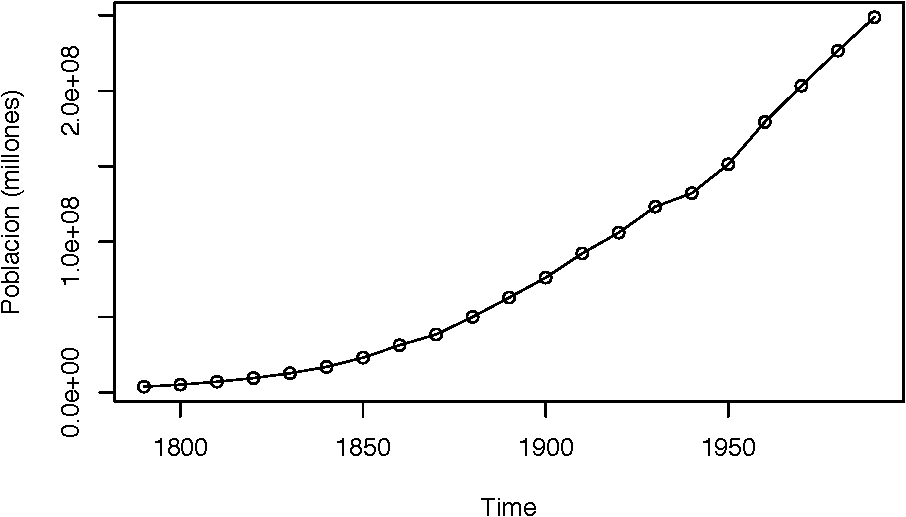
\includegraphics{Serie-de-Tiempo-en-R_files/figure-latex/unnamed-chunk-21-1.pdf}

Podemos notar del gráfico que la tendencia es creciente y parece tener
un comportamiento cuadrático, por lo que ajustando una función de la
forma \eqref{eq:eq-modelo-cuadratico} para la población de los datos USPOP
para \(1790\leq t\leq1980\) nos da los parámetros estimados

\[\hat{a}_0=2.101\times10^{10};\quad \hat{a}_1=-2.338\times10^{7}; \hat{a}_2=6.506\times10^{3}\]

En el gráfico siguiente se puede observar la curva ajustada y los datos
originales. Los valores estimados del proceso de ruido
\(\epsilon_t, 1790\leq t\leq1980\), son los residuales obtenidos por
sustracción de \(\hat{T}_t=\hat{a}_0+\hat{a}_1t+\hat{a}_2t^2\) de la
serie \(X_t\). La componente de tendencia \(T_t\) nos proporciona un
predictor natural de los valores futuros de \(X_t\). Por ejemplo si
deseamos estimar \(T_{1990}\) por su valor medio, obtenemos

\[T_{1990} = 2.4853\times10^8\]

para la población de EE.UU en 1990. Sin embargo si los residuales
\(\hat{\epsilon}_t\) están altamente correlacionados podemos ser capaces
de usar esos valores para dar una mejor estimación de \(T_{1990}\) y por
consiguiente de \(X_{1990}\).

\begin{Shaded}
\begin{Highlighting}[]
\NormalTok{x=}\KeywordTok{time}\NormalTok{(pop)}
\NormalTok{reg=}\KeywordTok{lm}\NormalTok{(pop}\OperatorTok{~}\NormalTok{x}\OperatorTok{+}\KeywordTok{I}\NormalTok{(x}\OperatorTok{^}\DecValTok{2}\NormalTok{),}\DataTypeTok{na.action=}\OtherTok{NULL}\NormalTok{)}
\KeywordTok{summary}\NormalTok{(reg)}
\end{Highlighting}
\end{Shaded}

\begin{verbatim}
## 
## Call:
## lm(formula = pop ~ x + I(x^2), na.action = NULL)
## 
## Residuals:
##      Min       1Q   Median       3Q      Max 
## -6947521  -358167   436285  1481410  3391761 
## 
## Coefficients:
##              Estimate Std. Error t value Pr(>|t|)    
## (Intercept)  2.10e+10   6.59e+08    31.9   <2e-16 ***
## x           -2.34e+07   6.98e+05   -33.5   <2e-16 ***
## I(x^2)       6.51e+03   1.85e+02    35.2   <2e-16 ***
## ---
## Signif. codes:  
## 0 '***' 0.001 '**' 0.01 '*' 0.05 '.' 0.1 ' ' 1
## 
## Residual standard error: 2770000 on 18 degrees of freedom
## Multiple R-squared:  0.999,  Adjusted R-squared:  0.999 
## F-statistic: 8.05e+03 on 2 and 18 DF,  p-value: <2e-16
\end{verbatim}

\begin{Shaded}
\begin{Highlighting}[]
\KeywordTok{plot}\NormalTok{(pop,}\DataTypeTok{type=}\StringTok{"o"}\NormalTok{,}\DataTypeTok{xlab=}\StringTok{"Años"}\NormalTok{,}\DataTypeTok{ylab=}\StringTok{"Poblacion (millones)"}\NormalTok{)}
\KeywordTok{lines}\NormalTok{(reg}\OperatorTok{$}\NormalTok{fitted.values,}\DataTypeTok{col=}\StringTok{"red"}\NormalTok{)}
\end{Highlighting}
\end{Shaded}

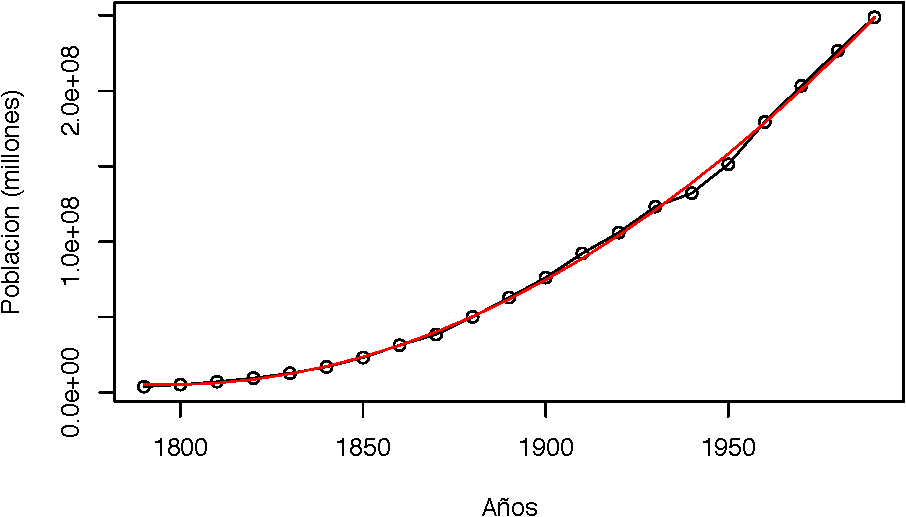
\includegraphics{Serie-de-Tiempo-en-R_files/figure-latex/unnamed-chunk-22-1.pdf}

\begin{center}\rule{0.5\linewidth}{\linethickness}\end{center}

\BeginKnitrBlock{example}
\protect\hypertarget{exm:ejemplo-poblacion-alemania-T1}{}{\label{exm:ejemplo-poblacion-alemania-T1}
}El archivo ``Population-North-Rhine-Westphalia.txt'' contiene la
población de la región North-Rhine-Westphalia (Alemania) en millónes
cada 5 años desde 1935 hasta 1980. Observando el gráfico podemos suponer
que la tendencia se puede ajustar por el modelo cúbico
\eqref{eq:eq-modelo-cubico}, esto es
\EndKnitrBlock{example}

\[T_t=\beta_0+\beta_1t+\beta_2t^2+\beta_3t^3\]

El código en R para el gráfico y el ajuste es

\begin{Shaded}
\begin{Highlighting}[]
\NormalTok{NRWpop=}\KeywordTok{read.table}\NormalTok{(}\StringTok{"data/Population-North-Rhine-Westphalia.txt"}\NormalTok{,}
                     \DataTypeTok{header =} \OtherTok{TRUE}\NormalTok{)}
\NormalTok{knitr}\OperatorTok{::}\KeywordTok{kable}\NormalTok{(}\KeywordTok{head}\NormalTok{(NRWpop,}\DataTypeTok{booktabs=}\OtherTok{TRUE}\NormalTok{,}
                  \DataTypeTok{caption=}\StringTok{"Población (en millones) de North-Rhine-Westphalia, Alemania, 1935-1980"}\NormalTok{))}
\end{Highlighting}
\end{Shaded}

\begin{tabular}{r|r}
\hline
Year & Population\\
\hline
1935 & 11772\\
\hline
1940 & 12059\\
\hline
1945 & 11200\\
\hline
1950 & 12926\\
\hline
1955 & 14442\\
\hline
1960 & 15694\\
\hline
\end{tabular}

\begin{Shaded}
\begin{Highlighting}[]
\KeywordTok{plot}\NormalTok{(NRWpop, }\DataTypeTok{type =} \StringTok{"b"}\NormalTok{,}\DataTypeTok{col=}\StringTok{"blue"}\NormalTok{,}\DataTypeTok{xlab =} \StringTok{"Años"}\NormalTok{,}\DataTypeTok{ylab =} \StringTok{"Población (millones)"}\NormalTok{)}
\CommentTok{# Modelo cúbico}
\NormalTok{t=NRWpop[,}\DecValTok{1}\NormalTok{]}
\NormalTok{pob=NRWpop[,}\DecValTok{2}\NormalTok{]}
\NormalTok{modelo=}\KeywordTok{lm}\NormalTok{(pob}\OperatorTok{~}\NormalTok{t}\OperatorTok{+}\KeywordTok{I}\NormalTok{(t}\OperatorTok{^}\DecValTok{2}\NormalTok{)}\OperatorTok{+}\KeywordTok{I}\NormalTok{(t}\OperatorTok{^}\DecValTok{3}\NormalTok{),}\DataTypeTok{na.action =} \OtherTok{NULL}\NormalTok{)}
\KeywordTok{summary}\NormalTok{(modelo)}
\end{Highlighting}
\end{Shaded}

\begin{verbatim}
## 
## Call:
## lm(formula = pob ~ t + I(t^2) + I(t^3), na.action = NULL)
## 
## Residuals:
##    Min     1Q Median     3Q    Max 
## -813.0 -199.2   67.1  275.6  493.8 
## 
## Coefficients:
##              Estimate Std. Error t value Pr(>|t|)   
## (Intercept)  2.11e+09   5.10e+08    4.13   0.0061 **
## t           -3.23e+06   7.81e+05   -4.14   0.0061 **
## I(t^2)       1.65e+03   3.99e+02    4.14   0.0061 **
## I(t^3)      -2.81e-01   6.79e-02   -4.14   0.0061 **
## ---
## Signif. codes:  
## 0 '***' 0.001 '**' 0.01 '*' 0.05 '.' 0.1 ' ' 1
## 
## Residual standard error: 472 on 6 degrees of freedom
## Multiple R-squared:  0.974,  Adjusted R-squared:  0.962 
## F-statistic: 76.2 on 3 and 6 DF,  p-value: 3.63e-05
\end{verbatim}

\begin{Shaded}
\begin{Highlighting}[]
\KeywordTok{lines}\NormalTok{(t,modelo}\OperatorTok{$}\NormalTok{fitted.values,}\DataTypeTok{col=}\StringTok{"red"}\NormalTok{)}
\end{Highlighting}
\end{Shaded}

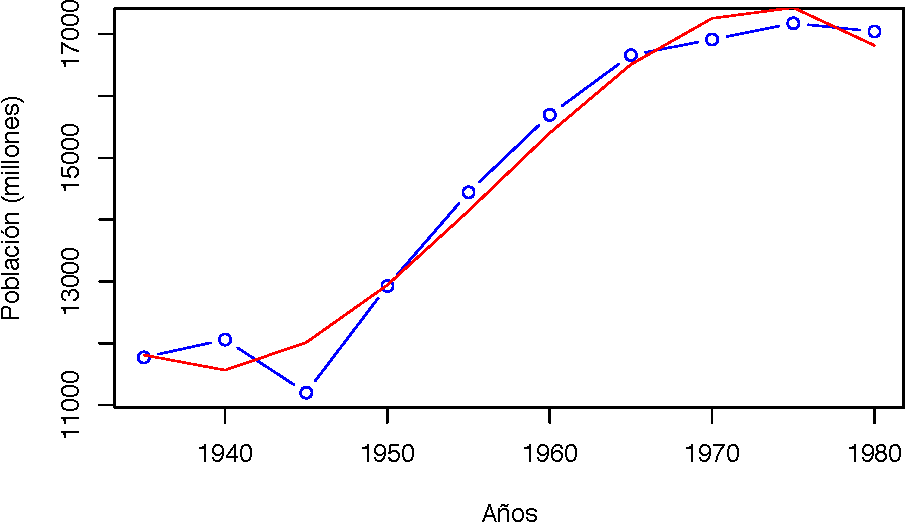
\includegraphics{Serie-de-Tiempo-en-R_files/figure-latex/unnamed-chunk-23-1.pdf}

La curva punteada en azul corresponde a los datos originales, la curva
en rojo corresponde al ajuste mediante el modelo cúbico.

\begin{center}\rule{0.5\linewidth}{\linethickness}\end{center}

\begin{enumerate}
\def\labelenumi{\arabic{enumi}.}
\setcounter{enumi}{1}
\tightlist
\item
  \textbf{Método T2: Suavizado por medio de un promedio móvil}. Sea
  \(q\) un entero no negativo y consideremos un promedio móvil de la
  forma
\end{enumerate}

\begin{equation}
W_t = \frac{1}{2q+1}\sum_{j=-q}^{q}X_{t+j}
\label{eq:eq-promedio-movil-orden-q}
\end{equation}

de un proceso \(\{X_t\}\) definido por \eqref{eq:eq-modelo-tendencia}.
Entonces para \(q+1\leq t\leq n-q\),

\begin{eqnarray}
W_t &=& \frac{1}{2q+1}\sum_{j=-q}^qT_{t+j}+\frac{1}{2q+1}\sum_{j=-q}^q\epsilon_{t+j}\\ \nonumber
    &\simeq& T_t \label{eq:eq-media-promedio-movil}
\end{eqnarray}

suponiendo que \(T_t\) es aproximadamente lineal sobre el intervalo
\([t-q,t+q]\) y que el promedio del término de error sobre este
intervalo es cercano a cero.

El promedio móvil entonces nos provee con el estimador

\begin{equation}
\hat{T}_t = \frac{1}{2q+1}\sum_{j=-q}^qX_{t+j},\quad q+1\leq t\leq n-q.
\label{eq:eq-estimador-promedio-movil}
\end{equation}

Dado que \(X_t\) es no observado para \(t\leq0\) o \(t\geq n\) no
podemos usar \eqref{eq:eq-estimador-promedio-movil} para \(t\leq q\) o
\(t>n-q\). Una forma de resolver este problema es haciendo \(X_t=X_1\)
para \(t<1\) y \(X_t=X_n\) para \(t>n\). A continuación presentamos un
ejemplo

\begin{center}\rule{0.5\linewidth}{\linethickness}\end{center}

\BeginKnitrBlock{example}
\protect\hypertarget{exm:ejem-huelgas-USA-T2}{}{\label{exm:ejem-huelgas-USA-T2}
}El gráfico siguiente muestra las huelgas ocurridas en EE.UU, de 1951 a
1980, según la Oficina de Estadísticas Laborales del Departamento de
Trabajo de los EE.UU.
\EndKnitrBlock{example}

A estos datos le aplicamos un promedio móvil de 5 puntos, la Figura
muestra la serie suavizada y el término de error estimado
\(\hat{\epsilon}_t = X_t - \hat{T}_t\) se muestra en la Figura
\ref{Grafico-tema3-residuales-huelga-USA}. Como era de esperarse ellos
no presentan una tendencia clara.

Las instrucciones en R para el suavizado y los gráficos son los
siguientes:

\begin{Shaded}
\begin{Highlighting}[]
\NormalTok{H=}\KeywordTok{read.table}\NormalTok{(}\StringTok{"data/Huelgas.txt"}\NormalTok{)}
\CommentTok{# Proemdio móvil por medio de la función "filter"}
\NormalTok{W=}\KeywordTok{filter}\NormalTok{(H[,}\DecValTok{2}\NormalTok{],}\DataTypeTok{sides=}\DecValTok{2}\NormalTok{,}\KeywordTok{rep}\NormalTok{(}\DecValTok{1}\OperatorTok{/}\DecValTok{5}\NormalTok{,}\DecValTok{5}\NormalTok{))}
\CommentTok{# Residuales de X_t}
\NormalTok{y=H[,}\DecValTok{2}\NormalTok{]}\OperatorTok{-}\NormalTok{W }
\CommentTok{# Graficos}
\KeywordTok{par}\NormalTok{(}\DataTypeTok{mfrow=}\KeywordTok{c}\NormalTok{(}\DecValTok{3}\NormalTok{,}\DecValTok{1}\NormalTok{))}
\KeywordTok{plot}\NormalTok{(H,}\DataTypeTok{xlab=}\StringTok{"años"}\NormalTok{,}\DataTypeTok{ylab=}\StringTok{"Huelgas"}\NormalTok{,}\DataTypeTok{type=}\StringTok{'b'}\NormalTok{,}
     \DataTypeTok{main =} \StringTok{"Huelgas en EE.UU., años 1951-1980"}\NormalTok{)}
\KeywordTok{plot}\NormalTok{(H[,}\DecValTok{1}\NormalTok{],W,}\DataTypeTok{xlab=}\StringTok{"años"}\NormalTok{,}\DataTypeTok{ylab=}\StringTok{"Huelgas"}\NormalTok{,}\DataTypeTok{type=}\StringTok{'b'}\NormalTok{,}
     \DataTypeTok{main =} \StringTok{"Promedio móvil de 5 puntos para los datos de Huelga"}\NormalTok{)}
\KeywordTok{plot}\NormalTok{(H[,}\DecValTok{1}\NormalTok{],y,}\DataTypeTok{xlab=}\StringTok{"años"}\NormalTok{,}\DataTypeTok{ylab=}\StringTok{"Residuales"}\NormalTok{,}\DataTypeTok{type=}\StringTok{'b'}\NormalTok{,}
     \DataTypeTok{main =} \StringTok{"Residuales e_t=X_t-T_t"}\NormalTok{)}
\end{Highlighting}
\end{Shaded}

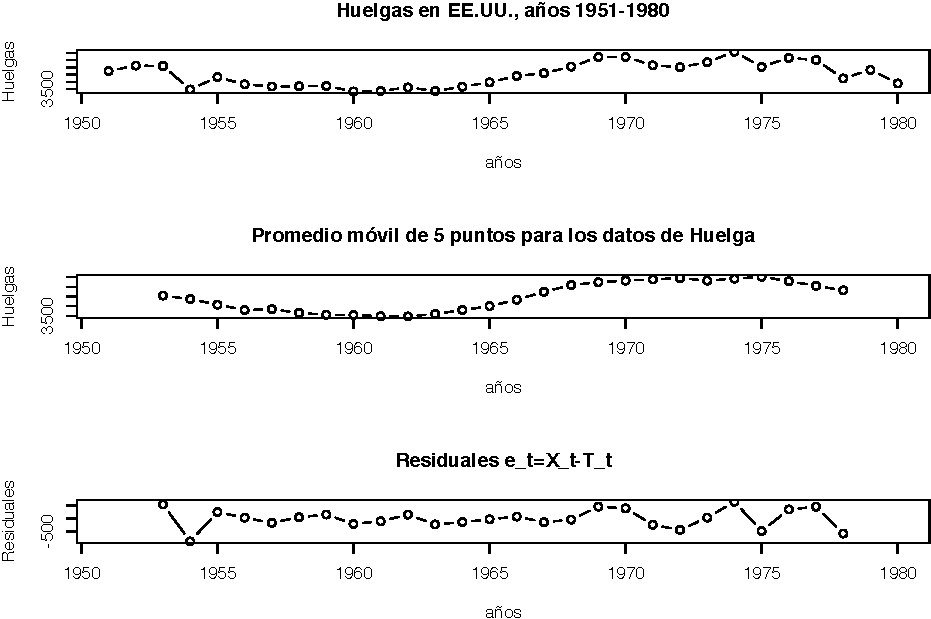
\includegraphics{Serie-de-Tiempo-en-R_files/figure-latex/unnamed-chunk-24-1.pdf}

\begin{center}\rule{0.5\linewidth}{\linethickness}\end{center}

Para cada valor fijo \(a\in[0,1]\), el promedio móvil de un lado
\(\hat{T}_t, t=1,\ldots,n\), definido por la recursión

\begin{equation}
  \hat{T}_t = aX_t+(1-a)\hat{T}_t,\quad t=2,\ldots,n
 \label{eq:eq-promedio-movil-1-lado-peso}
\end{equation}

y

\[\hat{T}_1=X_1,\]

se puede calcular usando la opción \emph{sides=1} en la función
\emph{filter} de R.

Es usual pensar como aplicación de la ecuación
\eqref{eq:eq-promedio-movil-1-lado-peso} como un suavizado exponencial,
dado que se sigue de la recursión que para
\(t\leq2, \hat{T}_t=\sum_{j=0}^{t-2}a(1-a)^jX_{t-j}+(1-a)^{t-1}X_1\), es
un promedio móvil con peso de \(X_t,X_{t-1},\ldots\), con pesos
decreciendo exponencialmente (excepto para el último término).

Es útil pensar en \(\{\hat{T}_t\}\) en (\emph{filter}) como un proceso
obtenido de \(\{X_t\}\) por aplicación de un operador lineal o filtro
lineal \(\hat{T}_t=\sum_{j=-\infty}^{\infty}a_jX_{t+j}\) con pesos
\(a_j=(2q+1)^{-1},-q\leq j\leq q\), y \(a_j=0,|j|>q\). Este filtro
particular es un filtro de ``paso-bajo'' ya que toma los datos
\(\{X_t\}\) y remueve la componente de rápida fluctuación (o de alta
frecuencia) \(\{\hat{\epsilon}_t\}\), para dejar el término de la
tendencia estimada de lenta variación \(\{\hat{T}_t\}\).

\begin{enumerate}
\def\labelenumi{\arabic{enumi}.}
\setcounter{enumi}{2}
\tightlist
\item
  \textbf{Método T3: Diferenciación para generar datos estacionarios}.
  En lugar de intentar remover el ruido por suavizado como en el Método
  T2, ahora intentaremos eliminar la tendencia por diferenciación.
  Definamos primero el operador diferencia \(\nabla\) por
\end{enumerate}

\begin{equation}
  \nabla x_t = x_t-x_{t-1}=(1-B)x_t,
\label{eq:eq-operador-diferencia}
\end{equation}

donde \(B\) es el operador de desplazamiento hacia atrás (\emph{backward
shift operator} en inglés),

\begin{equation}
  Bx_t=x_{t-1}.
\label{eq:eq-backward-shift-operator}
\end{equation}

Las potencias de los operadores \(B\) y \(\nabla\) se definen de manera
obvia, esto es, \(B^j(x_t)=x_{t-j}\) y
\(\nabla^j(x_t)=\nabla(\nabla^{j-1}(x_t)),j\geq1\) con
\(\nabla^0(x_t)=x_t\). Los polinomios en \(B\) y \(\nabla\) se manipulan
de la misma manera que las funciones polinómicas de variables reales.
Por ejemplo

\begin{eqnarray*}
  \nabla^2x_t &=& \nabla(\nabla x_t) = (1-B)(1-B)x_t = (1-2B+B^2)x_t \\
              &=& x_t-2x_{t-1}+x_{t-2}.
\end{eqnarray*}

Si el operador \(\nabla\) se aplica a una función con tendencia lineal
\(T_t=at+b\), entonces obtenemos la función constante \(\nabla T_t=a\).
De la misma manera cada tendencia polinomial de grado \(k\) se puede
reducir a una constante por aplicación del operador \(\nabla^k\).

Iniciando entonces con el modelo \(X_t=T_t+\epsilon_t\), donde
\(T_t=\sum_{j=0}^ka_jt^j\) y \(\epsilon_t\) es estacionario con media
cero, obtenemos

\[\nabla^kX_t = k!a_k+\nabla^k\epsilon_t,\]

un proceso estacionario con media \(k!a_k\). Esta consideración sugiere
la posibilidad, dada una sucesión \(\{X_t\}\) de datos, de aplicar el
operador \(\nabla\) repetidamente hasta conseguir una sucesión
\(\{\nabla^kX_t\}\) la cual puede ser apropiadamente modelada como una
realización de un proceso estacionario. Se encuentra a menudo en la
práctica que el orden \(k\) de diferenciación es bastante pequeño,
frecuentemente uno o dos. \footnote{Esto depende del hecho de que muchas
  funciones pueden ser aproximadas bastante bien, en un intervalo de
  longitud finita, por un polinomio de grado razonablemente bajo.}

\BeginKnitrBlock{example}
\protect\hypertarget{exm:ejem-diferenciacion-poblacion-usa-T2}{}{\label{exm:ejem-diferenciacion-poblacion-usa-T2}
}Aplicando esta técnica al ejemplo
\ref{exm:ejem-poblacion-usa-metodo-T1} de población de los EE.UU,
hallamos que dos operaciones de diferenciación son suficientes para
producir una serie sin aparente tendencia. Los datos diferenciados se
muestran en la Figura. Note que la magnitud de las fluctuaciones en
\(\nabla^2X_n\) se incrementa con el valor de \(n\). Este efecto se
puede suprimir tomando primero logaritmo natural, \(y_n=\ln X_n\) y
entonces aplicando el operador \(\nabla^2\) a la serie \(\{y_n\}\).
\EndKnitrBlock{example}

Las instrucciones en R son las siguientes

\begin{Shaded}
\begin{Highlighting}[]
\NormalTok{Dx=}\KeywordTok{diff}\NormalTok{(uspop,}\DataTypeTok{difference=}\DecValTok{2}\NormalTok{)}
\KeywordTok{plot}\NormalTok{(Dx,}\DataTypeTok{type=}\StringTok{"b"}\NormalTok{,}\DataTypeTok{xlab=}\StringTok{"Año"}\NormalTok{, }\DataTypeTok{ylab=}\StringTok{"Diferencias"}\NormalTok{)}
\end{Highlighting}
\end{Shaded}

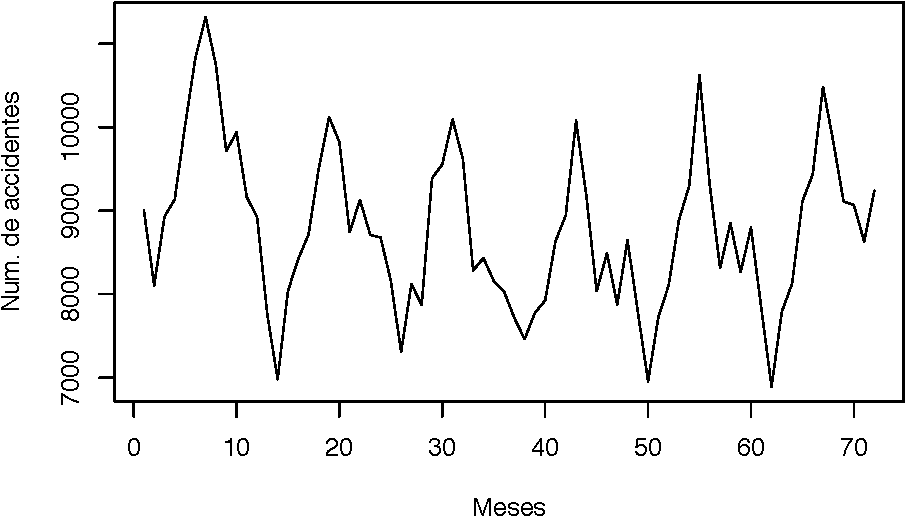
\includegraphics{Serie-de-Tiempo-en-R_files/figure-latex/unnamed-chunk-25-1.pdf}

\subsection{Estimación de la tendencia y la
estacionalidad}\label{estimacion-de-la-tendencia-y-la-estacionalidad}

Los métodos descritos para estimar y remover la tendencia pueden ser
adaptados de manera natural para estimar tanto la tendencia como la
estacionalidad en el modelo general

\begin{equation}
X_t = T_t + E_t + \epsilon_t
\end{equation}

donde \(\mathbb{E}(\epsilon_t)=0, E_{t+d}=E_t\) y \(\sum_{j=1}^dE_t=0\).
Ilustraremos estos métodos con referencia al siguiente ejemplo de
accidentes. El archivo ``Accidentes3.txt'' muestra el número de
accidentes mortales de automóviles mensual ocurridos en EE.UU., entre
los años 1973 y 1978. En la tabla siguiente se muestran los datos

\begin{Shaded}
\begin{Highlighting}[]
\NormalTok{X<-}\KeywordTok{read.table}\NormalTok{(}\StringTok{"data/Accidentes3.txt"}\NormalTok{, }\DataTypeTok{header =} \OtherTok{TRUE}\NormalTok{)}
\end{Highlighting}
\end{Shaded}

\begin{tabular}{l|r|r|r|r|r|r}
\hline
Mes & X1973 & X1974 & X1975 & X1976 & X1977 & X1978\\
\hline
Ene & 9007 & 7750 & 8162 & 7717 & 7792 & 7836\\
\hline
Feb & 8106 & 6981 & 7306 & 7461 & 6957 & 6892\\
\hline
Mar & 8928 & 8038 & 8124 & 7776 & 7726 & 7791\\
\hline
Abr & 9137 & 8422 & 7870 & 7925 & 8106 & 8129\\
\hline
May & 10017 & 8714 & 9387 & 8634 & 8890 & 9115\\
\hline
Jun & 10826 & 9512 & 9556 & 8945 & 9299 & 9434\\
\hline
\end{tabular}

En la figura podemos observar que los datos presentan claramente una
componente estacional con periodo \(d=12\).

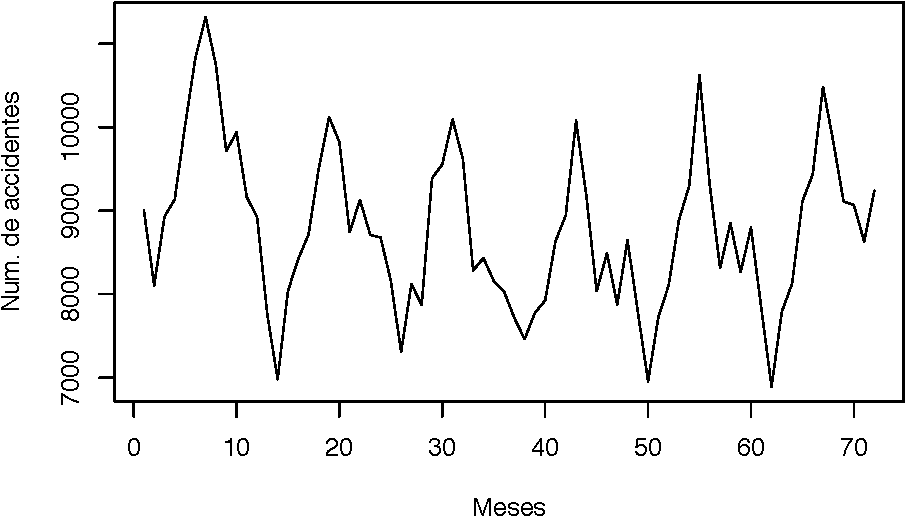
\includegraphics{Serie-de-Tiempo-en-R_files/figure-latex/unnamed-chunk-28-1.pdf}

Será conveniente para el primer método indexar los datos por mes y año.
Entonces \(X_{j,k}, j=1,\ldots,12, k=1,\ldots,6\) denotará el número de
muertes accidentales reportados para el \(j\)-ésimo mes del \(k\)-ésimo
año, \((1972+k)\). En otras palabras, definimos

\[X_{j,k}=X_{j+12(k-1)},\quad j=1,\ldots,12; k=1,\ldots,6.\]

\begin{enumerate}
\def\labelenumi{\arabic{enumi})}
\tightlist
\item
  \textbf{Método E1: Método de la tendencia pequeña}. Si la tendencia es
  pequeña (como en los datos de accidentes) no es irrazonable suponer
  que el término de la tendencia es constante, digamos \(T_k\) para el
  año \(k\). Dado que \(\sum_{j=1}^{12}E_j=0\), nos lleva al estimador
  insesgado natural para la tendencia
\end{enumerate}

\begin{equation}
\hat{T}_k = \frac{1}{12}\sum_{j=1}^{12}X_{j,k},
\label{eq:eq-estimador-Tj-accidentes}
\end{equation}

mientras que para la estacionalidad \(E_j, j=1,\ldots,12\) tenemos el
estimador

\begin{equation}
\hat{E}_j = \frac{1}{6}\sum_{k=1}^6(X_{j,k}-\hat{T}_k),
\label{eq:eq-estimador-Et-accidentes}
\end{equation}

el cual automáticamente satisface el requisito de que
\(\sum_{j=1}^{12}\hat{E}_j=0\). El término de error estimado para el mes
\(j\) del año \(k\) es por supuesto

\begin{equation}
\hat{\epsilon}_{j,k} = X_{j,k}-\hat{T}_k-\hat{E}_j, \quad j=1,\ldots,12; k=1,\ldots,6.
\label{eq:eq-estimador-epsilon-t-accidentes}
\end{equation}

La generalización de \eqref{eq:eq-estimador-Tj-accidentes} a
\eqref{eq:eq-estimador-epsilon-t-accidentes} para datos con estacionalidad
con un periodo distinto de 12 es bastante sencillo de realizar,
simplemente cambiamos 12 por el correspondiente valor de \(d\). Así, en
general, si tenemos \(n\) años (meses, semanas, días, etc.) y
estacionalidad con periodo \(d\), los estimadores seran:

Para la tendencia \(T_k\):

\begin{equation}
\hat{T}_k=\frac{1}{d}\sum_{j=1}^dX_{j,k}
\label{eq:eq-estimador-Tk-E1}
\end{equation}

Para la estacionalidad \(E_j\):

\begin{equation}
\hat{E}_j=\frac{1}{n}\sum_{k=1}^n(X_{j,k}-\hat{T}_k),\quad j=1,\ldots,d
\label{eq:eq-estimador-Ej-E1}
\end{equation}

Para el error

\begin{equation}
\hat{\epsilon}_{j,k}=X_{j,k}-\hat{T}_k-\hat{E}_j,\quad k=1,\ldots,n; j=1,\ldots,d.
\label{eq:eq-estimador-error-E1}
\end{equation}

Las Figuras siguientes muestran respectivamente las observaciones con la
tendencia removida \(X_{j,k}-\hat{T}_k\), la componente estacional
estimada \(\hat{E}_j\) y las observaciones con la tendencia y la
estacionalidad removida
\(\hat{\epsilon}_{j,k}=X_{j,k}-\hat{T}_k-\hat{E}_j\). En la última no se
observa una aparente tendencia o estacionalidad.

\begin{Shaded}
\begin{Highlighting}[]
\CommentTok{# Estimacion de la tendencia}
\NormalTok{Tk=}\KeywordTok{numeric}\NormalTok{(n}\OperatorTok{*}\NormalTok{d)}
\ControlFlowTok{for}\NormalTok{(k }\ControlFlowTok{in} \DecValTok{1}\OperatorTok{:}\NormalTok{n)}
\NormalTok{\{}
  \ControlFlowTok{for}\NormalTok{(j }\ControlFlowTok{in} \DecValTok{1}\OperatorTok{:}\NormalTok{d)}
\NormalTok{  \{}
\NormalTok{    Tk[(k}\OperatorTok{-}\DecValTok{1}\NormalTok{)}\OperatorTok{*}\NormalTok{d}\OperatorTok{+}\NormalTok{j]=Tk[(k}\OperatorTok{-}\DecValTok{1}\NormalTok{)}\OperatorTok{*}\NormalTok{d}\OperatorTok{+}\NormalTok{j]}\OperatorTok{+}\NormalTok{(}\DecValTok{1}\OperatorTok{/}\DecValTok{12}\NormalTok{)}\OperatorTok{*}\NormalTok{X[j,k}\OperatorTok{+}\DecValTok{1}\NormalTok{]}
\NormalTok{  \}}
\NormalTok{\}}
\CommentTok{# Grafico con la tendencia removida}
\KeywordTok{plot}\NormalTok{(V}\OperatorTok{-}\NormalTok{Tk,}\DataTypeTok{type =} \StringTok{"l"}\NormalTok{,}\DataTypeTok{xlab =} \StringTok{"Meses"}\NormalTok{,}\DataTypeTok{ylab =} \StringTok{"Num. de accidentes"}\NormalTok{,}
     \DataTypeTok{main =} \StringTok{"Accidentes mortales mensuales con la tendencia T_k removida"}\NormalTok{)}
\end{Highlighting}
\end{Shaded}

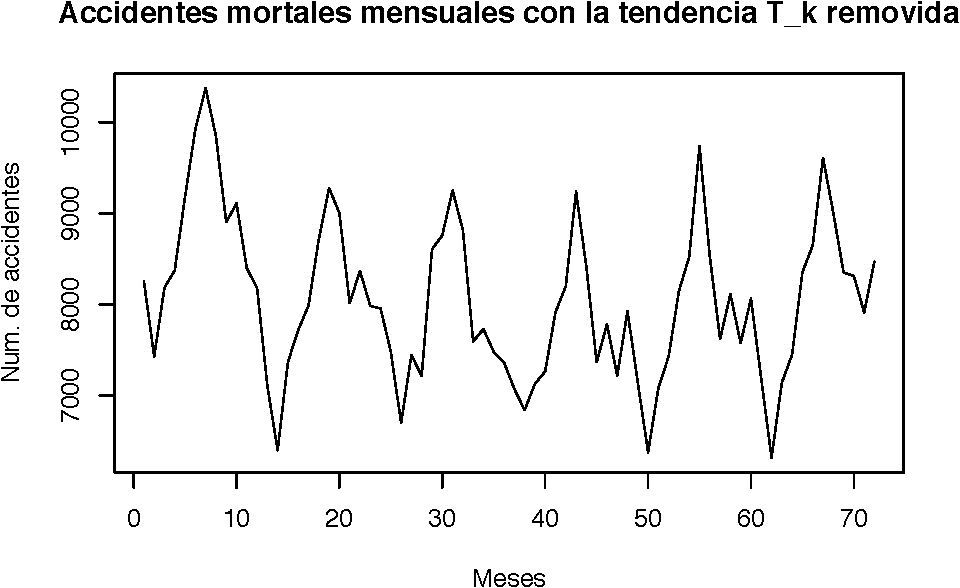
\includegraphics{Serie-de-Tiempo-en-R_files/figure-latex/unnamed-chunk-29-1.pdf}

\begin{Shaded}
\begin{Highlighting}[]
\CommentTok{# Estimacion de la estacionalidad}
\NormalTok{Ej=}\KeywordTok{numeric}\NormalTok{(n}\OperatorTok{*}\NormalTok{d)}
\ControlFlowTok{for}\NormalTok{(j }\ControlFlowTok{in} \DecValTok{1}\OperatorTok{:}\NormalTok{d)}
\NormalTok{\{}
\NormalTok{  aux=}\DecValTok{0}
  \ControlFlowTok{for}\NormalTok{(k }\ControlFlowTok{in} \DecValTok{1}\OperatorTok{:}\NormalTok{n)}
\NormalTok{  \{}
\NormalTok{    aux=aux}\OperatorTok{+}\NormalTok{(X[j,k}\OperatorTok{+}\DecValTok{1}\NormalTok{]}\OperatorTok{-}\NormalTok{Tk[(k}\OperatorTok{-}\DecValTok{1}\NormalTok{)}\OperatorTok{*}\NormalTok{d}\OperatorTok{+}\NormalTok{j])}
\NormalTok{  \}}
  \ControlFlowTok{for}\NormalTok{(k }\ControlFlowTok{in} \DecValTok{1}\OperatorTok{:}\NormalTok{n)}
\NormalTok{  \{}
\NormalTok{    Ej[(k}\OperatorTok{-}\DecValTok{1}\NormalTok{)}\OperatorTok{*}\NormalTok{d}\OperatorTok{+}\NormalTok{j]=(}\DecValTok{1}\OperatorTok{/}\NormalTok{n)}\OperatorTok{*}\NormalTok{aux}
\NormalTok{  \}}
\NormalTok{\}}
\CommentTok{# Grafico de la estacionalidad}
\KeywordTok{plot}\NormalTok{(Ej,}\DataTypeTok{type =} \StringTok{"l"}\NormalTok{,}\DataTypeTok{xlab =} \StringTok{"Meses"}\NormalTok{,}\DataTypeTok{ylab =} \StringTok{"Num. de accidentes"}\NormalTok{,}
     \DataTypeTok{main =} \StringTok{"Estacionalidad de los accidentes mortales mensuales"}\NormalTok{)}
\end{Highlighting}
\end{Shaded}

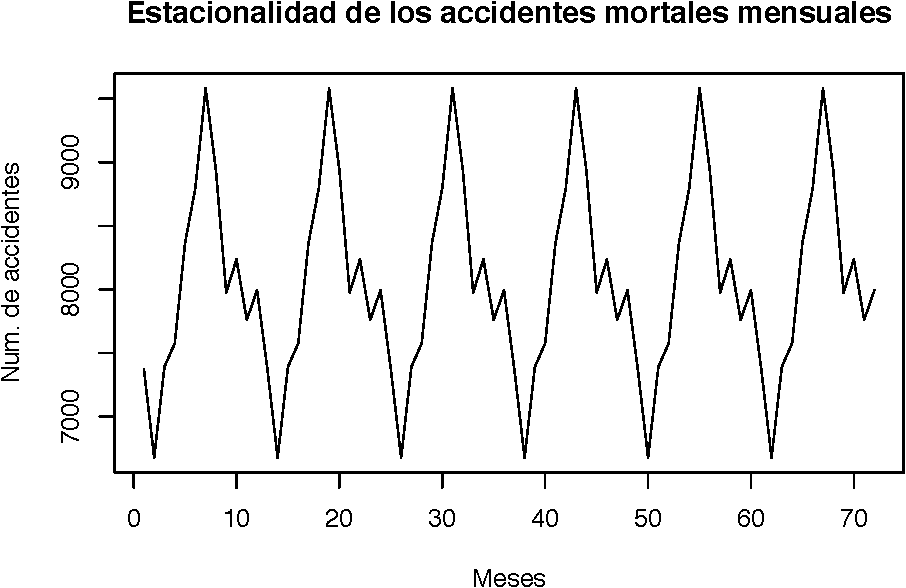
\includegraphics{Serie-de-Tiempo-en-R_files/figure-latex/unnamed-chunk-29-2.pdf}

\begin{Shaded}
\begin{Highlighting}[]
\CommentTok{# Estimacion del error}
\NormalTok{error=V}\OperatorTok{-}\NormalTok{Tk}\OperatorTok{-}\NormalTok{Ej}
\CommentTok{# Grafico del error estimado}
\KeywordTok{plot}\NormalTok{(error,}\DataTypeTok{type =} \StringTok{"l"}\NormalTok{,}\DataTypeTok{xlab =} \StringTok{"Meses"}\NormalTok{,}\DataTypeTok{ylab =} \StringTok{"Error estimado"}\NormalTok{,}
     \DataTypeTok{main =} \StringTok{"Error estimado de los accidentes mortales"}\NormalTok{)}
\KeywordTok{grid}\NormalTok{(}\DataTypeTok{col =} \StringTok{"darkgray"}\NormalTok{)     }
\end{Highlighting}
\end{Shaded}

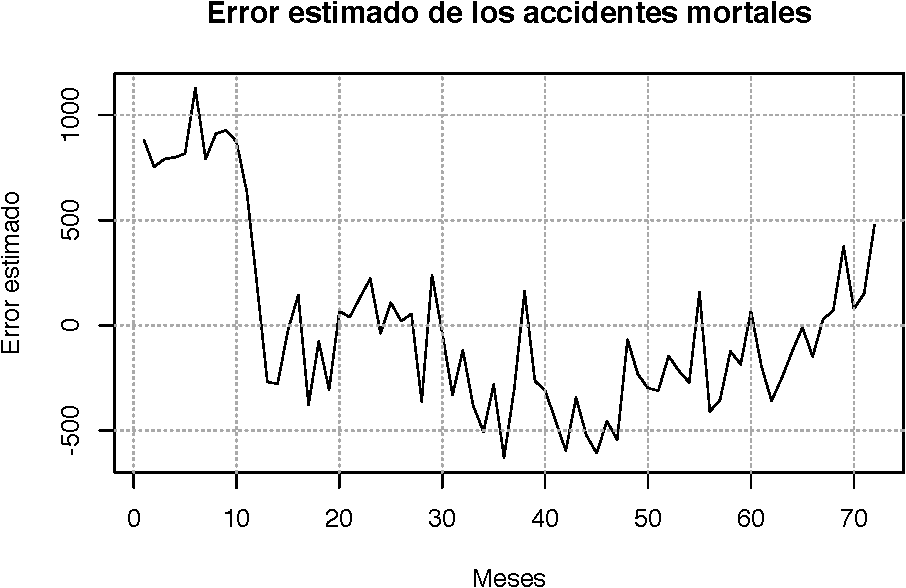
\includegraphics{Serie-de-Tiempo-en-R_files/figure-latex/unnamed-chunk-29-3.pdf}

\begin{enumerate}
\def\labelenumi{\arabic{enumi})}
\setcounter{enumi}{1}
\tightlist
\item
  \textbf{Método E2: Estimación por promedio móvil}. La siguiente
  técnica es preferible al Método E1 ya que no se basa en la suposición
  de que \(T_t\) es casi constante sobre cada ciclo estacional.
\end{enumerate}

Suponga que tenemos las observaciones \(\{x_1,\ldots,x_n\}\). Se estima
primero la tendencia aplicando un filtro de promedio móvil especialmente
elegido para eliminar la componente estacional y para amortiguar el
ruido. Si el periodo \(d\) es par, digamos \(d=2q\), entonces usamos

\begin{equation}
\hat{T}_t = (0.5x_{t-q} + x_{t-q+1} + \cdots + x_{t+q-1} + 0.5x_{t+q})/d, q<t\leq n-q.
\label{eq:eq-filtro-especial-metodo-S2}
\end{equation}

Si el periodo es impar, digamos \(d=2q+1\), entonces usamos el promedio
móvil simple \eqref{eq:eq-estimador-promedio-movil}. La
Figura\textasciitilde{}\ref{Grafico-tema3-accidentes-promedio-movil}
muestra la tendencia estimada \(\hat{T}_t\) para los datos de accidentes
mortales obtenido de \eqref{eq:eq-filtro-especial-metodo-S2}. También
muestra la tendencia constante a trozos obtenida por el Método S1.

El segundo paso, es estimar la componente estacional. Para cada
\(k=1,\ldots,d\), calculamos el promedio \(w_k\) de las desviaciones
\(\{(X_{k+jd}-\hat{T}_{k+jd}):q<k+jd\leq n-q\}\). Dado que este promedio
de desviaciones no necesariamente suma cero, estimamos la componente
estacional \(E_k\) como

\begin{equation}
\hat{E}_k = w_k -\frac{1}{d}\sum_{i=1}^dw_i,\quad i=1,\ldots,d,
\label{eq:eq-estimador-Et-metodo-S2}
\end{equation}

y \(\hat{E}_k=\hat{E}_{k-d},k>d\).

Los datos sin la componente estacional se definen entonces como la serie
original con la componente estacional removida, es decir,

\begin{equation}
d_t = X_t-\hat{E}_t,\quad t=1,\ldots,n.
\label{eq:eq-serie-destacionalizada}
\end{equation}

Finalmente, reestimamos la tendencia de \(\{d_t\}\) aplicando un filtro
de promedio móvil como se describió para los datos no estacionales o
fijando un polinomio a la serie \(\{d_t\}\). El término del ruido
estimado llega a ser entonces

\[\hat{\epsilon}_t = X_t - \hat{E}_t - \hat{E}_t, \quad t=1,\ldots,n.\]

Los resultados de aplicar los Métodos S1 y S2 a los datos de accidentes
mortales son casi iguales, dado que en este caso la constante a trozos y
el promedio móvil de \(T_t\) están razonablemente cercanos.

Una comparación de los valores estimados de \(E_k, k=1,\ldots,12\),
obtenido con ambos métodos se muestra en la
Tabla\textasciitilde{}\ref{Tabla-tema3-componentes-estacionales-estimadas}

\begin{longtable}[]{@{}lllllllllllll@{}}
\toprule
k & 1 & 2 & 3 & 4 & 5 & 6 & 7 & 8 & 9 & 10 & 11 & 12\tabularnewline
\midrule
\endhead
\(\hat{E}_t(S1)\) & -7434 & -1504 & -724 & -523 & 338 & 808 & 1665 & 961
& -87 & 197 & -321 & -67\tabularnewline
\(\hat{E}_t(S2)\) & -804 & -1522 & -737 & -526 & 343 & 746 & 1680 & 987
& -109 & 258 & -259 & -57\tabularnewline
\bottomrule
\end{longtable}

Componentes estacional estimadas para los datos de accidentes mortales

\begin{itemize}
\tightlist
\item
  \textbf{Método E3: Diferenciación a paso \(\mathbf{d}\)}. La técnica
  de diferenciación la cual aplicamos antes a datos no estacionales se
  pueden adaptar para lidiar con el caso estacional de periodo \(d\)
  introduciendo el operador de diferencia de paso \(d\) \(\nabla_d\)
  definido por
\end{itemize}

\begin{equation}
\nabla_dX_t = X_t-X_{t-d} = (1-B^d)X_t.
\label{eq:eq-operador-diferencia-paso-d}
\end{equation}

Este operador no debe confundirse con el operador \(\nabla^d = (1-B)^d\)
definido por (\ref{eq-operador-diferencia}).

Aplicando el operador \(\nabla_d\) al modelo

\[X_t = T_t + E_t + \epsilon_t,\] donde \(\{E_t\}\) tiene periodo \(d\),
obtenemos

\[\nabla_dX_t = T_t-T_{t-d} + \epsilon_t-\epsilon_{t-d},\]

lo cual nos da una descomposición de la diferencia \(\nabla_dX_t\) en
una componente de tendencia \((T_t-T_{t-d})\) y un término de ruido
\((\epsilon_t-\epsilon_{t-d})\). La tendencia \((T_t-T_{t-d})\) se puede
eliminar usando los métodos ya descritos, por ejemplo, aplicando alguna
potencia del operador \(\nabla\). La figura siguiente muestra el
resultado de aplicar el operador \(\nabla_{12}\) a los datos de
accidentes mortales.

\begin{Shaded}
\begin{Highlighting}[]
\CommentTok{# Operador Nabla_d, usamos la funcion diff con lag=12}
\NormalTok{NdX=}\KeywordTok{diff}\NormalTok{(V,}\DataTypeTok{lag=}\DecValTok{12}\NormalTok{)}
\KeywordTok{plot}\NormalTok{(NdX,}\DataTypeTok{type =} \StringTok{"l"}\NormalTok{)}
\end{Highlighting}
\end{Shaded}

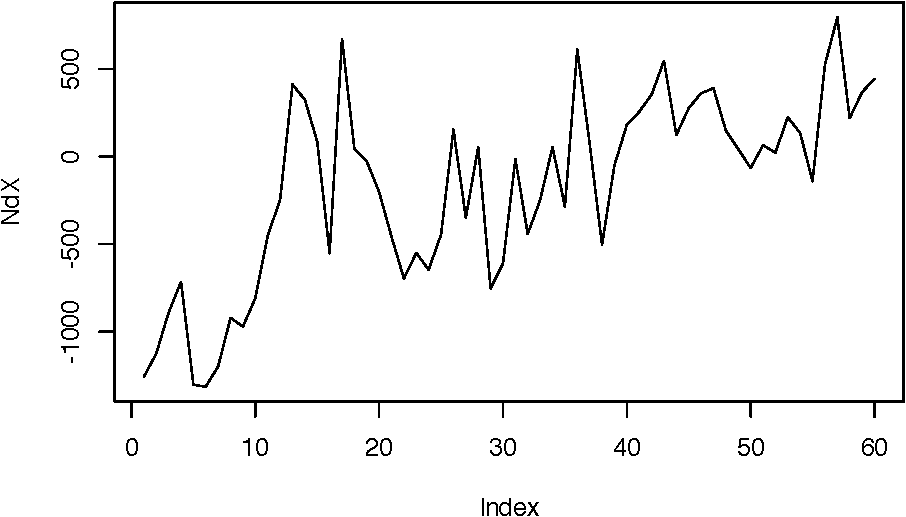
\includegraphics{Serie-de-Tiempo-en-R_files/figure-latex/unnamed-chunk-30-1.pdf}

La componente estacional evidente en la
Figura\textasciitilde{}\ref{Grafico-tema3-accidentes-USA} está ausente
en la Figura de \(\nabla_{12}X_t,13\leq t\leq72\). Sin embargo todavía
parece haber una tendencia decreciente. Si ahora aplicamos el operador
\(\nabla\) a \(\nabla_{12}X_t\) y graficamos las diferencias
\(\nabla\nabla_{12}X_t,t=14,\ldots,72\) obtenemos el gráfico mostrado en
la
Figura\textasciitilde{}\ref{Grafico-tema3-diferencia-diferencia-paso-12},
los cuales no tienen una aparente tendencia o componente estacional.

\begin{Shaded}
\begin{Highlighting}[]
\NormalTok{DNdX=}\KeywordTok{diff}\NormalTok{(NdX)}
\KeywordTok{plot}\NormalTok{(DNdX,}\DataTypeTok{type =} \StringTok{"l"}\NormalTok{)}
\end{Highlighting}
\end{Shaded}

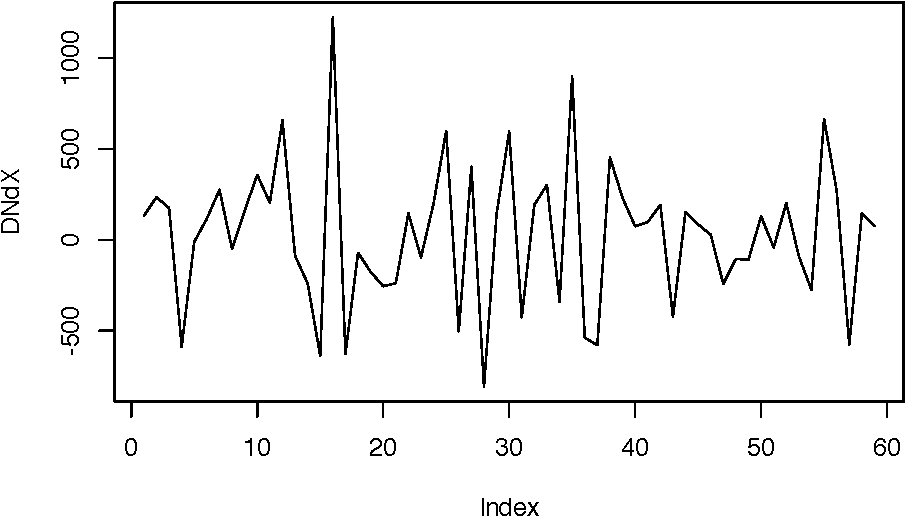
\includegraphics{Serie-de-Tiempo-en-R_files/figure-latex/unnamed-chunk-31-1.pdf}

\section{Estimación de la tendencia por regresión
clásica}\label{estimacion-de-la-tendencia-por-regresion-clasica}

Los modelos de regresión son importantes para modelos en el dominio de
tiempo y de frecuencia que discutiremos posteriormente. La idea
principal depende de poder expresar una serie respuesta \(X_t\) como una
combinación lineal de entradas \(z_{t_1},z_{t_2},\ldots,z_{t_q}\). La
estimación de los coeficientes \(\beta_1,\beta_2,\ldots,\beta_q\) de la
combinación por mínimos cuadrados proporciona un método para modelar
\(X_t\) en términos de las entradas.

\subsection{Regresión Clásica}\label{regresion-clasica}

Supongamos que tenemos \(X_t\), para \(t=1,2,\ldots,n\) influenciada por
una colección de series independientes
\(z_{t_1},z_{t_2},\ldots,z_{t_q}\), donde consideraremos primero que las
entradas son fijas y conocidas. Podemos expresar esta relación como

\begin{equation}
X_t=\beta_1z_{t_1}+\beta_2z_{t_2}+\cdots+\beta_qz_{t_q}+w_t
\label{eq:eq-regresion-lineal}
\end{equation}

donde \(\beta_1,\beta_2,\ldots,\beta_q\) son los coeficientes de
regresión fijos y desconocidos, \(\{w_t\}\) es un error aleatorio o un
proceso de ruido consistente de variables normales iid con media cero y
varianza \(\sigma_w^2\).

El modelo lineal descrito en \eqref{eq:eq-regresion-lineal} se puede
escribir de forma más general por medio de definir los vectores columna
\(\mathbf{z}_t=(z_{t_1},z_{t_2},\ldots,z_{t_q})^t\) y
\(\mathbf{\beta}=(\beta_1,\beta_2,\ldots,\beta_q)^t\) donde \(t\) denota
la traspuesta, así \eqref{eq:eq-regresion-lineal} será

\begin{equation}
X_t=\mathbf{\beta}^t\mathbf{z}_t+w_t
\label{eq:eq-regresion-lineal-2}
\end{equation}

donde \(w_t\sim iid(0,\sigma_w^2)\). Es natural considerar la estimación
de los coeficientes del vector \(\mathbf{\beta}\) minimizando la suma
residual de cuadrados

\begin{equation}
RSS=\sum_{t=1}^{n}(X_t-\mathbf{\beta}^t\mathbf{z}_t)^2
\label{eq:eq-suma-residual-cuadrados}
\end{equation}

con respecto a \(\beta_1,\beta_2,\ldots,\beta_q\). Minimizando RSS
obtenemos el estimador común de mínimos cuadrados. Esta minimización se
puede hacer por diferenciación de \eqref{eq:eq-suma-residual-cuadrados}
con respecto al vector \(\mathbf{\beta}\) o usando las propiedades de
proyección. En la notación anterior, obtenemos la ecuación normal

\begin{equation}
\left(\sum_{t=1}^{n}\mathbf{z}_t\mathbf{z}_t^t\right)\hat{\mathbf{\beta}}=\sum_{t=1}^{n}\mathbf{z}_tX_t
\label{eq:eq-regresion-lineal-normal}
\end{equation}

Definiendo la matriz
\(Z=(\mathbf{z}_1,\mathbf{z}_2,\ldots,\mathbf{z}_n)^t\) como una matriz
\(n\times q\) compuesta de \(n\) muestras de las variables de entradas y
el vector observado \(\mathbf{x}=(x_1,x_2,\ldots,x_n)^t\) se puede hacer
una simplificación de la notación. Esta identificación nos lleva a

\begin{equation}
(Z^tZ)\hat{\mathbf{\beta}}=Z^t\mathbf{x}
\label{eq:eq-regresion-matriz}
\end{equation}

y la solución es

\begin{equation}
\hat{\mathbf{\beta}}=(Z^tZ)^{-1}Z^t\mathbf{x},
\label{eq:eq-solucion-regresion-matriz}
\end{equation}

cuando la matriz \(Z^tZ\) es de rango \(q\). El residual minimizado de
suma de cuadrados \eqref{eq:eq-suma-residual-cuadrados} tiene la forma
matricial equivalente

\begin{eqnarray}
RSS&=&(\mathbf{x}-Z\hat{\mathbf{\beta}})^t(\mathbf{x}-Z\hat{\mathbf{\beta}})\\ \nonumber
&=&\mathbf{x}^t\mathbf{x}-\hat{\mathbf{\beta}}^tZ^t\mathbf{x}\\ \nonumber
&=&\mathbf{x}^t\mathbf{x}-\mathbf{x}^tZ(Z^tZ)^{-1}Z^t\mathbf{x}.
\label{eq:eq-suma-residual-cuadrados-matricial}
\end{eqnarray}

El estimador común de mínimos cuadrados es insesgado, esto es,
\(\mathbb{E}(\hat{\mathbf{\beta}})=\mathbf{\beta}\), y tiene la menor
varianza de todos los estimadores insesgados lineales.

Si los errores \(w_t\) son normalmente distribuidos (Gaussianos),
\(\hat{\mathbf{\beta}}\) es también el estimador de máxima verosimilitud
para \(\mathbf{\beta}\) y es normalmente distribuido con

\begin{eqnarray}
\text{cov}(\hat{\mathbf{\beta}})&=&\sigma_w^2\left(\sum_{t=1}^{n}\mathbf{z}_t\mathbf{z}_t^t\right)^{-1}\\ \nonumber
&=&\sigma_w^2(Z^tZ)^{-1}\\ \nonumber
&=&\sigma_w^2C,
\label{eq:eq-covarianza-beta-estimado}
\end{eqnarray}

donde

\begin{equation}
C=(Z^tZ)^{-1}.
\label{eq:eq-matriz-C}
\end{equation}

Un estimador insesgado para la varianza \(\sigma_w^2\) es

\begin{equation}
s_w^2=\frac{RSS}{n-q}
\label{eq:eq-estimador-insesgado-varianza}
\end{equation}

contrastado con el estimador de máxima verosimilitud
\(\hat{\sigma}_w^2=RSS/n\) el cual tiene divisor \(n\). Bajo la
suposición de que \(s_w^2\) tiene distribución proporcional a una
variable aleatoria chi-cuadrado con \(n-q\) grados de libertad,
\(\chi_{n-q}^2\), e independiente de \(\hat{\beta}\), se sigue que

\begin{equation}
t_{n-q}=\frac{(\hat{\beta}_i-\beta_i)}{s_w\sqrt{c_{ii}}}
\label{eq:eq-estadistico-t}
\end{equation}

tiene distribución \(t\)-de Student con \(n-q\) grados de libertad;
\(c_{ii}\) denota el \(i\)-ésimo elemento de la diagonal de \(C\), como
se definió en \eqref{eq:eq-matriz-C}.

Hay varios modelos que podemos utilizar de manera de seleccionar el
mejor subconjunto de variables independientes. Suponga que tenemos un
modelo que sólo considera un subconjunto \(q_1<q\) de variables
independientes \(\mathbf{z}_{1t}=(z_{t_1},z_{t_2},\ldots,z_{t_q1})^t\)
que influencian a la variable \(X_t\), así el modelo

\begin{equation}
X_t=\mathbf{\beta}_1^t\mathbf{z}_{1t}+w_t
\label{eq:eq-modelo-regresion-reducido}
\end{equation}

llega a ser la hipótesis nula, donde
\(\mathbf{\beta}_1=(\beta_1,\beta_2,\ldots,\beta_{q1})^t\) es un
subconjunto de los coeficientes de las \(q\) variables originales.
Podemos contrastar el modelo reducido
\eqref{eq:eq-modelo-regresion-reducido} contra el modelo completo
\eqref{eq:eq-regresion-lineal-2} comparando el residual de la suma de
cuadrados bajo los dos modelos usando el estadístico \(F\)

\begin{equation}
F_{q-q1,n-q}=\frac{RSS_1-RSS}{RSS}\frac{n-q}{q-q1}
\label{eq:eq-estadistico-F-residuales}
\end{equation}

el cual tiene distribución \(F\) con \(q-q1\) y \(n-q\) grados de
libertad cuando \eqref{eq:eq-estadistico-F-residuales} es el modelo
correcto. La información envuelta en la prueba se resume en una tabla de
Análisis de Varianza (ANOVA) como la mostrada en la Tabla siguiente para
este caso particular. La diferencia en el numerador es llamada regresión
de la suma de cuadrados.

\begin{longtable}[]{@{}llll@{}}
\toprule
\begin{minipage}[b]{0.10\columnwidth}\raggedright\strut
Fuente\strut
\end{minipage} & \begin{minipage}[b]{0.07\columnwidth}\raggedright\strut
g.l\strut
\end{minipage} & \begin{minipage}[b]{0.25\columnwidth}\raggedright\strut
Suma de cuadrados\strut
\end{minipage} & \begin{minipage}[b]{0.23\columnwidth}\raggedright\strut
Medias Cuadrados\strut
\end{minipage}\tabularnewline
\midrule
\endhead
\begin{minipage}[t]{0.10\columnwidth}\raggedright\strut
\(z_{t,q_1+1},\ldots,z_{t,q}\)\strut
\end{minipage} & \begin{minipage}[t]{0.07\columnwidth}\raggedright\strut
\(q-q_1\)\strut
\end{minipage} & \begin{minipage}[t]{0.25\columnwidth}\raggedright\strut
\(SS_{reg}=RSS_1-RSS\)\strut
\end{minipage} & \begin{minipage}[t]{0.23\columnwidth}\raggedright\strut
\(MS_{reg}=SS_{reg}/(q-q_1)\)\strut
\end{minipage}\tabularnewline
\begin{minipage}[t]{0.10\columnwidth}\raggedright\strut
Error\strut
\end{minipage} & \begin{minipage}[t]{0.07\columnwidth}\raggedright\strut
\(n-q\)\strut
\end{minipage} & \begin{minipage}[t]{0.25\columnwidth}\raggedright\strut
\(RSS\)\strut
\end{minipage} & \begin{minipage}[t]{0.23\columnwidth}\raggedright\strut
\(s_e^2=RSS/(n-q)\)\strut
\end{minipage}\tabularnewline
\begin{minipage}[t]{0.10\columnwidth}\raggedright\strut
Total\strut
\end{minipage} & \begin{minipage}[t]{0.07\columnwidth}\raggedright\strut
\(n-q_1\)\strut
\end{minipage} & \begin{minipage}[t]{0.25\columnwidth}\raggedright\strut
\(RSS_1\)\strut
\end{minipage} & \begin{minipage}[t]{0.23\columnwidth}\raggedright\strut
\strut
\end{minipage}\tabularnewline
\bottomrule
\end{longtable}

En términos de la Tabla, por convención escribimos el estadístico \(F\)
dado en \eqref{eq:eq-estadistico-F-residuales} como el radio de dos medias
cuadrados, obteniéndose

\begin{equation}
F_{q-q1,n-q}=\frac{M S_{reg}}{s_w^2}.
\label{eq:eq-estadistico-F-radio-medias}
\end{equation}

Un caso de especial interés es para \(q_1=1\) y \(z_{1t}=1\), así el
modelo en \eqref{eq:eq-modelo-regresion-reducido} es \[X_t=\beta_1+w_t\] y
la proporción de variación explicada por las otras variables es

\begin{equation}
R_{xz}^2=\frac{RSS_0-RSS}{RSS_0},
\label{eq:eq-proporcion-variacion-explicada}
\end{equation}

donde la suma residual de cuadrados bajo el modelo reducido dada por

\begin{equation}
RSS_0=\sum_{t=1}^{n}(X_t-\bar{X})^2
\label{eq:eq-suma-residual-reducido}
\end{equation}

es precisamente la suma de desviaciones al cuadrado de la media
\(\bar{X}\). La medida \(R_{xz}^2\) es la correlación múltiple cuadrado
entre \(X_t\) y \(z_{t2},z_{t3},\ldots,z_{tq}\).

Las técnicas discutidas se pueden usar para hacer comparación entre
varios modelos. Estas pruebas han sido usadas en el pasado en una manera
gradual, donde las variables son añadidas o suprimidas cuando los
valores de la prueba \(F\) exceden o fallan en exceder algunos niveles
predeterminados. El procedimiento, llamado regresión múltiple por pasos,
es útil para conseguir un conjunto de variables que sea de utilidad. Una
manera alternativa es enfocándose en un procedimiento para selección del
modelo que no sea secuencial, sino simplemente evaluar cada modelo en
base a sus propios méritos.

Suponga que consideramos un modelo de regresión con \(k\) coeficientes y
denotemos el estimador de máxima verosimilitud para la varianza como

\begin{equation}
\hat{\sigma}_k^2=\frac{RSS_k}{n}
\label{eq:eq-estimador-emv-varianza}
\end{equation}

donde \(RSS_k\) denota la suma residual de cuadrados bajo el modelo con
\(k\) coeficientes de regresión. Entonces, Akaike (1969, 1973, 1974)
sugirió medir la bondad del ajuste para este modelo en particular
equilibrando el error del ajuste contra el número de parámetros en el
modelo; definiendo lo siguiente

\BeginKnitrBlock{definition}[Criterio de Información de Akaike (AIC)]
\protect\hypertarget{def:defi-AIC}{}{\label{def:defi-AIC} \iffalse (Criterio
de Información de Akaike (AIC)) \fi{} }El Criterio de Información de
Akaike se define como

\begin{equation}
AIC=\ln\hat{\sigma}_k^2+\frac{n+2k}{n}
\label{eq:eq-AIC}
\end{equation}

donde \(\hat{\sigma}_k^2\) está dado por
\eqref{eq:eq-estimador-emv-varianza} y \(k\) es el número de parámetros en
el modelo
\EndKnitrBlock{definition}

\begin{center}\rule{0.5\linewidth}{\linethickness}\end{center}

El \emph{criterio de información de Akaike} (AIC) es una medida de la
calidad relativa de un modelo estadístico, para un conjunto dado de
datos. Como tal, el AIC proporciona un medio para la selección del
modelo. El valor de \(k\) que minimiza \(AIC\) especifica el mejor
modelo. La idea es que la minimización de \(\hat{\sigma}_k^2\) sea
razonablemente objetiva, excepto que decrezca monótonamente cuando \(k\)
crece. Por lo tanto, debemos penalizar la variación del error por un
término proporcional al número de parámetros. La elección del término de
penalización dado por \eqref{eq:eq-AIC} no es único.

\chapter{Modelos de series de tiempo}\label{modelos-de-series-de-tiempo}

Como indicamos en el capítulo anterior el objetivo principal en el
análisis de series de tiempo es desarrollar modelos matemáticos que
provean una descripción apropiada para los datos muestrales. Recordando
las definiciones \ref{def:defi-serie-tiempo} y
\ref{def:defi-proceso-estocastico} podemos describir los modelos
generales útiles para la descripción de series de tiempo

\section{Modelos Estocásticos}\label{modelos-estocasticos}

\subsection{Procesos Estocásticos}\label{procesos-estocasticos}

De la definición de procesos estocásticos (Definición
\ref{def:defi-proceso-estocastico}), las variables aleatorias de la
familia (medibles para todo \(t\in T\)) son funciones de la forma
\[x(\omega,t):\Omega\times T\to\mathbb{R}\] Para \(T=\mathbb{N}\),
tenemos un proceso en \emph{tiempo discreto} y para
\(T\subset\mathbb{R}\) tenemos un proceso en \emph{tiempo continuo}. En
lo que respecta a este libro, consideraremos como subconjunto de índices
\(T=(0,\infty)\).

Como ya indicamos, usaremos la notación \(X_t\) para denotar la
realización de un proceso estocástico \(x_t(\omega*)\) cuando no haya
lugar a confución. De esta forma, adoptaremos sin pérdida de
generalidad, el conjunto de índices habitual de las series de tiempo en
el ámbito de las finanzas y economía \(I=(1,T)\).

De lo anterior, se tiene que los procesos estocásticos suelen ser
descritos mediante su distribución conjunta de probabilidades, de manera
que la relación que existe entre una realización y un proceso
estocástico es análoga a la existente entre la muestra y la población en
el análisis estadístico clásico.

\subsection{Momentos, Varianza, Covarianza y
Correlación}\label{momentos-varianza-covarianza-y-correlacion}

\BeginKnitrBlock{definition}
\protect\hypertarget{def:defi-esperanza-varianza-procesos}{}{\label{def:defi-esperanza-varianza-procesos}
}El \textbf{valor esperado} y \textbf{varianza} de un proceso
estocástico están dados por

\begin{equation}
\mathbb{E}(x_t)=\int_{\Omega}x(\omega,t)dP(\omega),\quad t\in[0,T]
\label{eq:eq-esperanza-proceso}
\end{equation}

y

\begin{equation}
Var(x_t)=\mathbb{E}(x_t-\mathbb{E}(x_t))^2,\quad t\in[0,T]
\label{eq:eq-varianza-proceso}
\end{equation}

siempre que las integrales existan y sean finitas.
\EndKnitrBlock{definition}

\BeginKnitrBlock{definition}
\protect\hypertarget{def:defi-k-esimo-momento-proceso}{}{\label{def:defi-k-esimo-momento-proceso}
}El \textbf{\(k\)-ésimo momento} de \(x_t\), con \(k\geq1\), se define
como \(\mathbb{E}(x_t^k)\) para todo \(t\in[0,t]\).
\EndKnitrBlock{definition}

\BeginKnitrBlock{definition}
\protect\hypertarget{def:defi-funcion-covarianza-proceso}{}{\label{def:defi-funcion-covarianza-proceso}
}La \textbf{función de covarianza} del proceso para dos instantes de
tiempo \(t\) y \(s\) está dada por
\[\gamma(t,s)=Cov(x_t,x_s)=\mathbb{E}[(x_t-\mathbb{E}(x_t))(x_s-\mathbb{E}(x_s))]\]
La cantidad \(x_t-x_s\) es llamada el proceso de \emph{incrementos}
desde \(s\) a \(t\), con \(s<t\).
\EndKnitrBlock{definition}

\subsection{Variación de un proceso}\label{variacion-de-un-proceso}

Sea \(P_n=\{0=t_0<t_1<\cdots<t_i<\cdots<t_n=t\}\) una partición
cualquiera del intervalos \([0,t]\) en \(n\) subintervalos y denotemos
por \[||P_n||=\max\{j=0,1,\ldots,n-1(t_{j+1}-t_j)\}\] el tamaño de paso
máximo de discretización de la partición \(P_n\).

\BeginKnitrBlock{definition}
\protect\hypertarget{def:defi-variacion-proceso}{}{\label{def:defi-variacion-proceso}
}La \textbf{variación} del proceso \(x\) se define como

\begin{equation}
V_t(x)=p-\lim_{||P_n||}\sum_{k=0}^{n-1}|x_{t_{k+1}}-x_{t_k}|
\label{eq:eq-variacion-proceso}
\end{equation}

Si \(x\) es diferenciable, entonces \(V_t(x)=\int_0^t|x'(u)|du\). Si
\(V_t(X)<\infty\), entonces decimos que \(x\) es de \emph{variación
acotada} en \([0,t]\). Si es cierto para todo \(t\geq0\), entonces
decimos que \(x\) tiene \emph{variación acotada}.
\EndKnitrBlock{definition}

\BeginKnitrBlock{definition}
\protect\hypertarget{def:defi-variacion-acotada}{}{\label{def:defi-variacion-acotada}
}La \textbf{variación cuadrática} de un proceso estocástico \(x\),
denotada por \([x,x]_t\), se define como

\begin{equation}
[x,x]_t = p-\lim_{||P_n||}\sum_{k=0}^{n-1}|x_{t_{k+1}}-x_{t_k}|^2
\label{eq:eq-variacion-acotada-proceso}
\end{equation}
\EndKnitrBlock{definition}

Para procesos estocásticos con trayectorias continua, el límite existe,
y en dicho caso usamos la notación \(\langle x,x\rangle_t\) y podemos
definirla alternativamente como

\begin{equation}
\langle x,x\rangle_t = p-\lim_{n\to\infty}\sum_{k=1}^{2^n}\left(x_{\min(t,k/2^n)} - x_{\min(t,(k-1)/2^n)}\right)^2
\label{eq:eq-variacion-acotada-proceso-2}
\end{equation}

Si \(x\) es continuo y tiene variación acotada cuadrática finita,
entonces su variación total es infinita. Note que \(V_t(x)\) y
\([x,x]_t\) son también procesos estocásticos.

\subsection{Martingalas}\label{martingalas}

En teoría de probabilidad, un proceso estocástico de tipo
\textbf{martingala} (galicismo de \emph{martingale}) es todo proceso
caracterizado por no tener deriva. Este tipo de procesos estocásticos
reciben su nombre de la estrategia de la martingala, un método de
apuestas que tuvo cierta fama en el siglo XVIII. La estrategia de la
martingala consiste en volver a apostar por el total perdido al momento
de incurrir en una pérdida en un juego de azar,. En la nueva apuesta, el
jugador tiene la posibilidad de recobrar todas sus pérdidas, por lo que
podría parecer que a largo plazo la esperanza de ganancia con esta
estrategia se mantienen constantes y a favor del jugador. De hecho,
estadísticamente es así: el capital medio del jugador (esto es, el
dinero que el jugador tiene a su disposición para jugar) se mantiene
constante. El problema reside en que, al incurrir en sucesivas pérdidas,
el jugador que siga la estrategia de la martingala se ve obligado a
apostar de nuevo cantidades cada vez mayores (las pérdidas acumuladas),
que tienden a crecer exponencialmente. Al cabo de unos pocos ciclos de
apuestas, el jugador, cuyos recursos son habitualmente muy inferiores a
los de la banca, se ve arruinado al ser incapaz de apostar de nuevo por
el total de sus pérdidas. Evitar jugadores que intenten seguir la
estratega de la martingala es de todos modos una de las razones por las
que los casinos actuales establecen límites máximos de apuesta.

La estrategia de la martingala se popularizó en el siglo XVIII con fama
de ser una estrategia ingenua y propia de mentes simples, puesto que
aunque en apariencia es infalible, sin embargo, está abocada a arruinar
al jugador. Recibe el nombre de los habitantes de la localidad francesa
de \emph{Martigues} (martingales en francés), situada en las cercanías
de Marsella, que por aquel entonces tenían fama de ser ingenuos y
simplones.

El concepto de la martingala en la teoría de probabilidades fue
introducido por \emph{Paul Pierre Lévy}, y una gran parte del desarrollo
original de la teoría la realizó \emph{Joseph Leo Doob}. Parte de la
motivación para ese esfuerzo era demostrar la inexistencia de
estrategias de juego infalibles.

El concepto fue inmediatamente aplicado al análisis de procesos
bursátiles. Uno de los resultados más importantes de la matemática
financiera es, precisamente, que un mercado perfecto sin posibilidades
de arbitraje es una martingala.

\BeginKnitrBlock{definition}
\protect\hypertarget{def:defi-filtracion}{}{\label{def:defi-filtracion} }Sea
\((\omega,\mathcal{F},P)\) un espacio de probabilidad. Una
\textbf{filtración} \(\{\mathcal{F}_t,t\geq0\}\) es una familia
creciente de sub-\(\sigma\)-álgebras de \(\mathcal{F}\) indexadas por
\(t\geq0\); es decir, para cada \(s,t>0\) tal que \(s<t\), se tiene
\(\mathcal{F}_s\subset\mathcal{F}_t\) con
\(\mathcal{F}_0=\{\Omega,\emptyset\}\).
\EndKnitrBlock{definition}

Para cada proceso estocástico \(\{x_t\}_{t\geq0}\) y para cada \(t\),
podemos asociar una \(\sigma\)-álgebra denotada por
\(\mathcal{F}_t=\sigma\{x_s:0\leq s\leq t\}\), y que además es la
\(\sigma\)-álgebra generada por \(x\); es decir, la \(\sigma\)-álgebra
más pequeña (minimal) de \(\mathcal{F}\) que hace a \(x(s,\omega)\)
medible para cada \(0\leq s\leq t\).

\BeginKnitrBlock{definition}
\protect\hypertarget{def:defi-proceso-adaptado}{}{\label{def:defi-proceso-adaptado}
}Dado un proceso estocástico \(\{X_t\}_{t\geq0}\) y una filtración
\(\{\mathcal{F}_t, t\geq0\}\) (no necesariamente la que genera \(X\)),
el proceso \(X\) se denomina \textbf{adaptado} a
\(\{\mathcal{F}_t, t\geq0\}\) (\(\mathcal{F}_t\)-adaptado) si para cada
\(t\geq0\), \(X(t)\) es \(\mathcal{F}_t\)-medible.
\EndKnitrBlock{definition}

En otras palabras \(X=\{X_t\}_{t\geq0}\) es \(\mathcal{F}_t\)-adaptado
cuando el valor de \(X_t\) en el tiempo \(t\) solo depende de la
información contenida en la realización hasta el instante \(t\).

Dado un espacio de probabilidad \((\Omega,\mathcal{F},P)\) y una
filtración \(\{\mathcal{F}_t,t\geq0\}\), entonces definimos el
\textbf{espacio de probabilidad filtrado} a la cuaterna
\((\Omega,\mathcal{F},\{\mathcal{F}_t\}_{t\geq0},P)\).

\BeginKnitrBlock{definition}
\protect\hypertarget{def:defi-martingala}{}{\label{def:defi-martingala} }Sea
\((\Omega,\mathcal{F},\{\mathcal{F}_t\}_{t\geq0},P)\) un espacio de
probabilidad filtrado. Un proceso \(X_t\) con \(t\in T\),
\(T\subseteq\mathcal{R}\) un conjunto de índices, es una
\textbf{martingala} relativo a la filtración
\(\{\mathcal{F}_t,t\geq0\}\), si

\begin{enumerate}
\def\labelenumi{\arabic{enumi})}
\item
  \(X_t\) es adaptado a la filtración \(\{\mathcal{F}_t,t\geq0\}\)
\item
  \(X_t\) es integrable, es decir, \(\mathbb{E}|X_t|<\infty\),
\item
  Para cualesquieras \(s\) y \(t\) con \(s<t\),
  \(\mathbb{E}(X_t|\mathcal{F}_s)=X_s\) c.s.
\end{enumerate}

Decimos que el proceso es una \textbf{submartingala} si
\[\mathbb{E}(X_t|\mathcal{F}_s)\geq X_s \text{ c.s.}\] Decimos que es
una \textbf{supermartingala} si
\[\mathbb{E}(X_t|\mathcal{F}_s)\leq X_s \text{ c.s.}\]
\EndKnitrBlock{definition}

\BeginKnitrBlock{example}
\protect\hypertarget{exm:unnamed-chunk-32}{}{\label{exm:unnamed-chunk-32}
}Sean \(X_0,X_1,\ldots,X_n\) variables aleatorias iid tal que
\(\mathbb{E}(X_1)=\mu\) y sean

\begin{eqnarray*}
M_0 &=& X_0 \\
M_1 &=& X_0+X_1 \\
\vdots & & \vdots \\
M_n &=& X_0+X_1+\cdots+X_n
\end{eqnarray*}

La sucesión de variables aleatorias \(M_n\) se llama \textbf{paseo
aleatorio} y es una supermartingala si \(\mu\leq0\), una martingala si
\(\mu=0\) y una submartingala si \(\mu\geq0\).

Es fácil demostrarlo, sencillamente usamos el hecho de que
\[M_{n+1}=M_n+X_{n+1}\] y que \(M_n\) y \(X_{n+1}\) son independientes.
Podemos generar tal proceso en \textbf{R}.
\EndKnitrBlock{example}

\begin{Shaded}
\begin{Highlighting}[]
\NormalTok{n=}\DecValTok{100}
\NormalTok{mu=}\DecValTok{0}
\NormalTok{sigma=}\DecValTok{1}
\NormalTok{X=}\KeywordTok{rnorm}\NormalTok{(n,mu,sigma)}
\NormalTok{M=}\KeywordTok{cumsum}\NormalTok{(X)}
\KeywordTok{plot}\NormalTok{(M,}\DataTypeTok{type =} \StringTok{"l"}\NormalTok{,}\DataTypeTok{xlab =} \StringTok{"t"}\NormalTok{,}\DataTypeTok{ylab =} \StringTok{"M_n"}\NormalTok{)}
\end{Highlighting}
\end{Shaded}

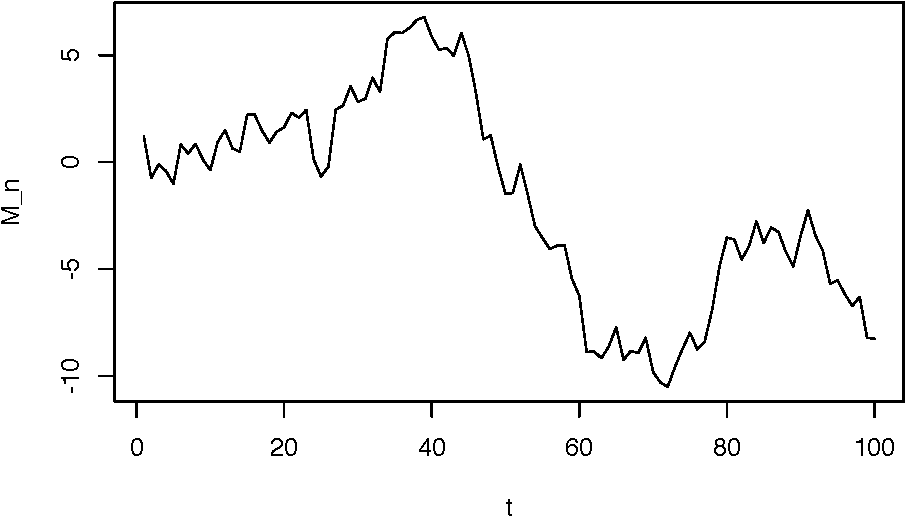
\includegraphics{Serie-de-Tiempo-en-R_files/figure-latex/unnamed-chunk-33-1.pdf}
\BeginKnitrBlock{example}[Precio de acciones]
\protect\hypertarget{exm:unnamed-chunk-34}{}{\label{exm:unnamed-chunk-34}
\iffalse (Precio de acciones) \fi{} }Sean \(Y_0,Y_1,\ldots,Y_n\)
variables aleatorias independientes y positivas. Supongamos que una
acción tiene precio \(M_0\) a tiempo \(t=0\).
\EndKnitrBlock{example}

Un modelo común para modelar el precio de la acción en tiempo \(t=n\) es

\[M_{n+1}=M_nY_n\]

donde \((Y_n-1)\times100\) representa (en porcentaje) la variabilidad de
la acción. Usando las propiedades de esperanza condicional (Apéndice),
es muy sencillo demostrar que

\[\mathbb{E}(M_{n+1}|M_0,\ldots,M_n)=M_n\mathbb{E}(Y_n)\]

En particular, si \(Y_1,\ldots,Y_n\) son idénticamente distribuidas con
\(\mathbb{E}(Y_1)=\mu\) tenemos que \(M_n\) es

\begin{itemize}
\item
  Una \textbf{martingala} si \(\mu=1\)
\item
  Una \textbf{submartingala} si \(\mu>1\)
\item
  Una \textbf{supermartingala} si \(\mu<1\).
\end{itemize}

Dos modelos bien conocidos de lo anterior son

\begin{enumerate}
\def\labelenumi{\arabic{enumi})}
\tightlist
\item
  Modelo \textbf{Black-Scholes discreto}.
\end{enumerate}

Sean \(Y_1,\ldots,Y_n\) definidas por

\[Y_n=e^{Z_n}\]

donde \(Z_1,\ldots,Z_n\) son variables aleatorias independientes
normales \(N(\mu,\sigma^2)\).

\begin{enumerate}
\def\labelenumi{\arabic{enumi})}
\setcounter{enumi}{1}
\tightlist
\item
  \textbf{Modelo Binomial}.
\end{enumerate}

Sean \(Y_1,\ldots,Y_n\) definidas por

\[P(Y_i=(1+t)e^{-r})=p\quad\text{ y }\quad P(Y_i=(1+t)^{-1}e^{-r})=1-p\]

La constante \(r\) es la tasa de interés y los factores \((1+t)\) y
\((1+t)^{-1}\) modelan las variaciones del mercado y garantizan que el
precio tiene la forma \(M_0(1+t)^ye^{-nr}\), con \(|y|\leq n\). La
volatilidad del precio está asociada a \(p\).

\BeginKnitrBlock{definition}
\protect\hypertarget{def:defi-proceso-cuadrado-integrable}{}{\label{def:defi-proceso-cuadrado-integrable}
}Una variable aleatoria \(X\) es \textbf{cuadrado integrable} si
\(\mathbb{E}(X^2)<\infty\). Un proceso estocástico \(X_t\) en el
intervalo \([0,T]\), donde \(T\) puede ser infinito, es \textbf{cuadrado
integrable} si

\begin{equation}
\sup_{t\in[0,T]}\mathbb{E}(X_t^2)<\infty
\label{eq:eq-proceso-cuadrado-integrable}
\end{equation}

es decir, si sus segundos momentos son acotados.
\EndKnitrBlock{definition}

\BeginKnitrBlock{definition}
\protect\hypertarget{def:defi-proceso-uniforme-integrable}{}{\label{def:defi-proceso-uniforme-integrable}
}Un proceso estocástico \(X_t, 0\leq t\leq T\) se dice que es
\textbf{uniformemente integrable} si
\[\mathbb{E}(|X_t|\mathbf{1}_{\{|X_t|>n\}})\] converge a 0 cuando
\(n\to\infty\) uniformemente en \(t\).
\EndKnitrBlock{definition}

\subsection{Propiedad de Markov}\label{propiedad-de-markov}

La propiedad de Markov establece que si conocemos el estado actual de un
proceso estocástico, entonces el comportamiento futuro de dicho proceso
es independiente de su pasado. Un proceso \(X_t\) tiene la
\emph{propiedad de Markov} si la distribución condicional del proceso
\(X_t\) dado el proceos en el instante \(X_t=x\), no depende de los
valores pasados.

\BeginKnitrBlock{definition}
\protect\hypertarget{def:defi-proceso-markov}{}{\label{def:defi-proceso-markov}
}\(X\) es un \textbf{proceso de Markov} si para cualquier \(t\) y
\(s>0\),
\[P(X_{t+s}\leq y|\mathcal{F}_t) = P(X_{t+s}\leq y|X_t) \text{ c.s.}\]
donde \(\mathcal{F}_t\) es la \(\sigma\)-álgebra generada por el proceso
hasta el tiempo \(t\).
\EndKnitrBlock{definition}

\BeginKnitrBlock{definition}
\protect\hypertarget{def:defi-funcion-transicion-probabilidad}{}{\label{def:defi-funcion-transicion-probabilidad}
}La \textbf{función de transición de probabilidad} de un proceso \(X\)
se define como \[P(y,t,x,s) = P(X_y\leq y|X_s\leq x)\] la función de
distribución condicional del proceso en el instante \(t\), dado que éste
está en el punto \(x\) en el instante \(s<t\).
\EndKnitrBlock{definition}

La propiedad de Markov implica una expresión que resulta muy útil en
términos de la esperanza condicional por la \(\sigma\)-álgebra de
eventos, la cual es válida tanto para procesos en tiempo discreto como
en tiempo continuo.

Las definiciones y propiedades anteriores son temas de estudio de gran
importancia y con una amplia teoría matemática que está fuera del
alcance de este libro, pero lo que hemos descrito es suficiente para el
objetivo del mismo.

\section{Modelos lineales}\label{modelos-lineales}

Los modelos lineales proporcionan un enfoque natural que permite
analizar el comportamiento de los procesos estocásticos o series de
tiempo y en especial a lo referente a finanzas y economía. En esta
sección discutiremos la estructura de dependencia, autocorrelación,
modelización y predicción de los modelos lineales teóricos, con los
correspondientes comandos en \textbf{R} para generar y nalaizar dichos
procesos.

\subsection{Proceso de Ruido Blanco}\label{proceso-de-ruido-blanco}

\BeginKnitrBlock{definition}
\protect\hypertarget{def:defi-ruido-blanco}{}{\label{def:defi-ruido-blanco}
}Un proceso \(\{w_t\}\) se denomina \textbf{ruido blanco} (white noise)
de media 0 y varianza \(\sigma^2\) si satisface

\begin{eqnarray*}
\mathbb{E}(w_t) &=& 0,\quad Var(w_t)=\sigma_w^2<\infty \\
Cov(w_t,w_{t-k}) &=& 0, \forall k\neq0
\end{eqnarray*}
\EndKnitrBlock{definition}

Las series de tiempo generadas de esta manera son muy usadas como
modelos para ruido en aplicaciones de ingeniería. La designación
\emph{``blanco''} se origina de la analogía con la luz blanca e indica
que todos los posibles períodos de oscilación están presentes con igual
intensidad.

En particular, una sucesión de variables aleatorias iid con media 0 y
varianza \(\sigma_w^2\) representa un caso especial de un proceso de
ruido blanco. Este proceso lo denotaremos por
\(w_t\sim WN(0,\sigma_w^2)\). Un muy usado ruido blanco es el
\textbf{ruido blanco gaussiano}, donde las \(w_t\) son variables
aleatorias normales o gaussianas con media 0 y varianza \(\sigma_w^2\) y
denotadas como \(w_t\sim iidN(0,\sigma_w^2)\).

La función de media de un ruido blanco es trivial, es decir
\[\mu_w=\mathbb{E}(w_t)=0.\] Calculemos la función de autocovarianza de
\(w_t\)

\begin{eqnarray*}
\gamma_w(s,t) &=& \mathbb{E}[(w_s-\mu_s)(w_t-\mu_t)] \\
      &=& \mathbb{E}[w_sw_t] \\
      &=& \begin{cases}
            \sigma_w^2, &\text{ si }s=t \\
            0, &\text{ si }s\neq t
          \end{cases}
\end{eqnarray*}

La última igualdad se sigue del hecho de que \(w_s\) y \(w_t\) son
no-correlacionados para \(s\neq t\) por lo que
\(\mathbb{E}(w_sw_t) = \mathbb{E}(w_s)\mathbb{E}(w_t)=0\).

\BeginKnitrBlock{example}[Estacionaridad de un ruido blanco]
\protect\hypertarget{exm:unnamed-chunk-35}{}{\label{exm:unnamed-chunk-35}
\iffalse (Estacionaridad de un ruido blanco) \fi{} }La función de
autocovarianza de un ruido blanco es fácil de evaluar como
\[\gamma_w(h) = \mathbb{E}(w_{t+h}w_t) = \begin{cases}
                                          \sigma_w^2,&\text{ si }h=0\\
                                          0,&\text{ si }h\neq0
                                         \end{cases}\] donde
\(\sigma_w^2\) es la varianza del ruido blanco. Esto significa que la
serie es \emph{débilmente estacionaria} o \emph{estacionaria}. Si las
variables de ruido blanco también son gaussianas, el proceso es
\emph{estrictamente estacionario}, como se pueder ver evaluando (2.10)
usando la relación (2.2).
\EndKnitrBlock{example}

\begin{Shaded}
\begin{Highlighting}[]
\CommentTok{#-----------------------------------------}
\CommentTok{# Ruidos blancos}
\CommentTok{#-----------------------------------------}
\CommentTok{# Uniforme [0,1]}
\NormalTok{wu=}\KeywordTok{runif}\NormalTok{(}\DecValTok{500}\NormalTok{,}\DecValTok{0}\NormalTok{,}\DecValTok{1}\NormalTok{)}
\CommentTok{# Gaussiano}
\NormalTok{wn=}\KeywordTok{rnorm}\NormalTok{(}\DecValTok{500}\NormalTok{,}\DecValTok{0}\NormalTok{,}\DecValTok{1}\NormalTok{)}
\CommentTok{# Graficos}
\KeywordTok{par}\NormalTok{(}\DataTypeTok{mfrow=}\KeywordTok{c}\NormalTok{(}\DecValTok{2}\NormalTok{,}\DecValTok{1}\NormalTok{))}
\KeywordTok{plot}\NormalTok{(wu,}\DataTypeTok{type =} \StringTok{"l"}\NormalTok{,}\DataTypeTok{xlab =} \StringTok{"Num. de observaciones"}\NormalTok{,}
     \DataTypeTok{main =} \StringTok{"Ruido blanco uniforme en [0,1]"}\NormalTok{)}
\KeywordTok{plot}\NormalTok{(wn,}\DataTypeTok{type =} \StringTok{"l"}\NormalTok{,}\DataTypeTok{xlab =} \StringTok{"Num. de observaciones"}\NormalTok{,}
     \DataTypeTok{main =} \StringTok{"Ruido blanco gaussiano"}\NormalTok{)}
\end{Highlighting}
\end{Shaded}

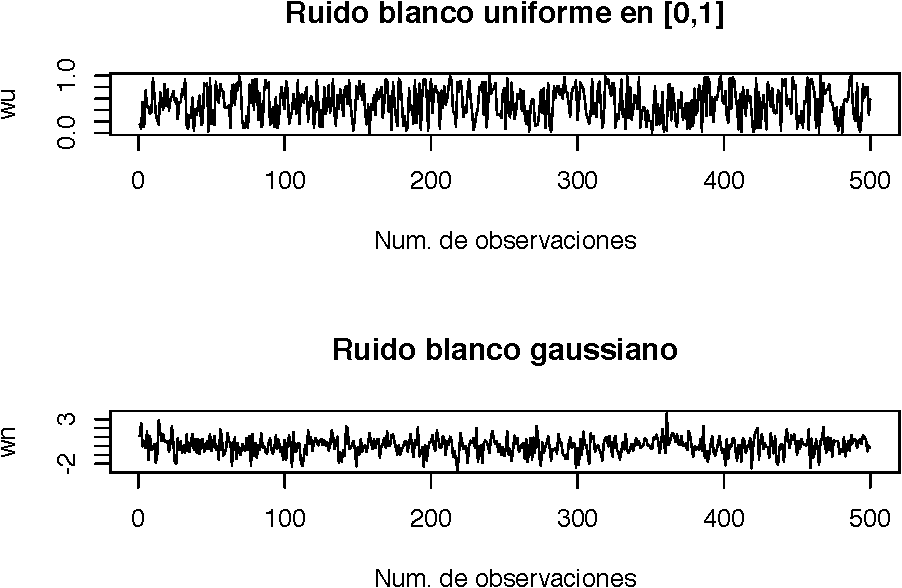
\includegraphics{Serie-de-Tiempo-en-R_files/figure-latex/unnamed-chunk-36-1.pdf}

\begin{Shaded}
\begin{Highlighting}[]
\CommentTok{# Funciones de autocovarianza (ACF)}
\KeywordTok{acf}\NormalTok{(wu)}
\KeywordTok{acf}\NormalTok{(wn)}
\end{Highlighting}
\end{Shaded}

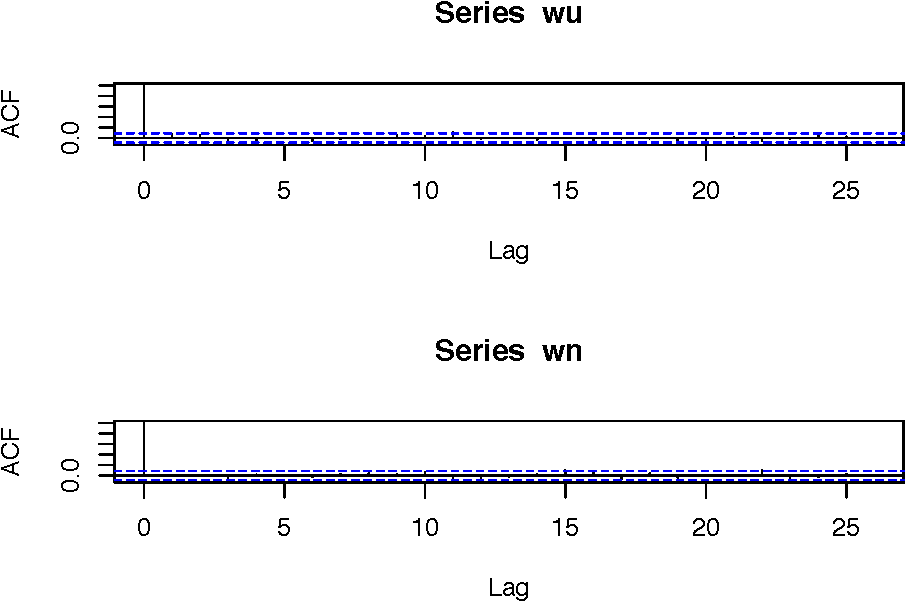
\includegraphics{Serie-de-Tiempo-en-R_files/figure-latex/unnamed-chunk-36-2.pdf}

\BeginKnitrBlock{example}
\protect\hypertarget{exm:ejem-promedio-movil-ruido-blanco}{}{\label{exm:ejem-promedio-movil-ruido-blanco}
}Podemos reemplazar las series de ruido blanco \(w_t\) por un promedio
móvil que suavice la serie. Por ejemplo, consideremos la serie \(w_t\)
en la ecuación ( ) y reemplacémosla por un promedio móvil de 3 puntos,
dado por

\begin{equation}
v_t = \frac{1}{3}(w_{t-1}+w_t+w_{t+1})
\label{eq:eq-promedio-movil-ruido-blanco}
\end{equation}

lo cual nos da una serie suavizada. Tomando la serie del ejemplo
anterior y usando la función `filter' de \textbf{R} se obtienen los
gráficos siguientes:
\EndKnitrBlock{example}

\begin{Shaded}
\begin{Highlighting}[]
\CommentTok{#------------------------------------------}
\CommentTok{# Promedio movil}
\CommentTok{#------------------------------------------}
\CommentTok{# Uniforme}
\NormalTok{vu=}\KeywordTok{filter}\NormalTok{(wu,}\DataTypeTok{sides =} \DecValTok{2}\NormalTok{,}\KeywordTok{rep}\NormalTok{(}\DecValTok{1}\OperatorTok{/}\DecValTok{3}\NormalTok{,}\DecValTok{3}\NormalTok{))}
\KeywordTok{par}\NormalTok{(}\DataTypeTok{mfrow=}\KeywordTok{c}\NormalTok{(}\DecValTok{2}\NormalTok{,}\DecValTok{1}\NormalTok{),}\DataTypeTok{mar=}\KeywordTok{c}\NormalTok{(}\DecValTok{3}\NormalTok{,}\DecValTok{4}\NormalTok{,}\DecValTok{3}\NormalTok{,}\DecValTok{2}\NormalTok{))}\CommentTok{#}
\KeywordTok{plot.ts}\NormalTok{(wu,}\DataTypeTok{xlab=}\StringTok{" "}\NormalTok{,}\DataTypeTok{ylab=}\StringTok{"Ruido blanco unif."}\NormalTok{)}
\KeywordTok{plot.ts}\NormalTok{(vu,}\DataTypeTok{ylim=}\KeywordTok{c}\NormalTok{(}\DecValTok{0}\NormalTok{,}\DecValTok{1}\NormalTok{),}\DataTypeTok{ylab=}\StringTok{"Promedio móvil")}
\end{Highlighting}
\end{Shaded}

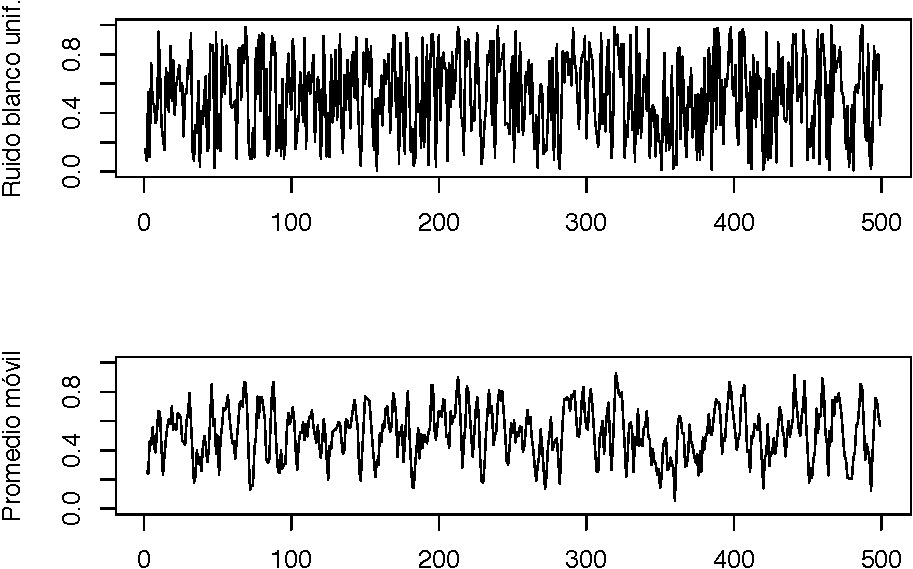
\includegraphics{Serie-de-Tiempo-en-R_files/figure-latex/unnamed-chunk-37-1.pdf}

\begin{Shaded}
\begin{Highlighting}[]
\CommentTok{# Gaussiano}
\NormalTok{vn=}\KeywordTok{filter}\NormalTok{(wn,}\DataTypeTok{sides =} \DecValTok{2}\NormalTok{,}\KeywordTok{rep}\NormalTok{(}\DecValTok{1}\OperatorTok{/}\DecValTok{3}\NormalTok{,}\DecValTok{3}\NormalTok{))}
\KeywordTok{par}\NormalTok{(}\DataTypeTok{mfrow=}\KeywordTok{c}\NormalTok{(}\DecValTok{2}\NormalTok{,}\DecValTok{1}\NormalTok{),}\DataTypeTok{mar=}\KeywordTok{c}\NormalTok{(}\DecValTok{3}\NormalTok{,}\DecValTok{4}\NormalTok{,}\DecValTok{3}\NormalTok{,}\DecValTok{2}\NormalTok{))}
\KeywordTok{plot.ts}\NormalTok{(wn,}\DataTypeTok{xlab=}\StringTok{" "}\NormalTok{,}\DataTypeTok{ylab=}\StringTok{"Ruido blanco gauss."}\NormalTok{)}
\KeywordTok{plot.ts}\NormalTok{(vn,}\DataTypeTok{ylim=}\KeywordTok{c}\NormalTok{(}\OperatorTok{-}\DecValTok{3}\NormalTok{,}\DecValTok{3}\NormalTok{),}\DataTypeTok{ylab=}\StringTok{"Promedio móvil")}
\end{Highlighting}
\end{Shaded}

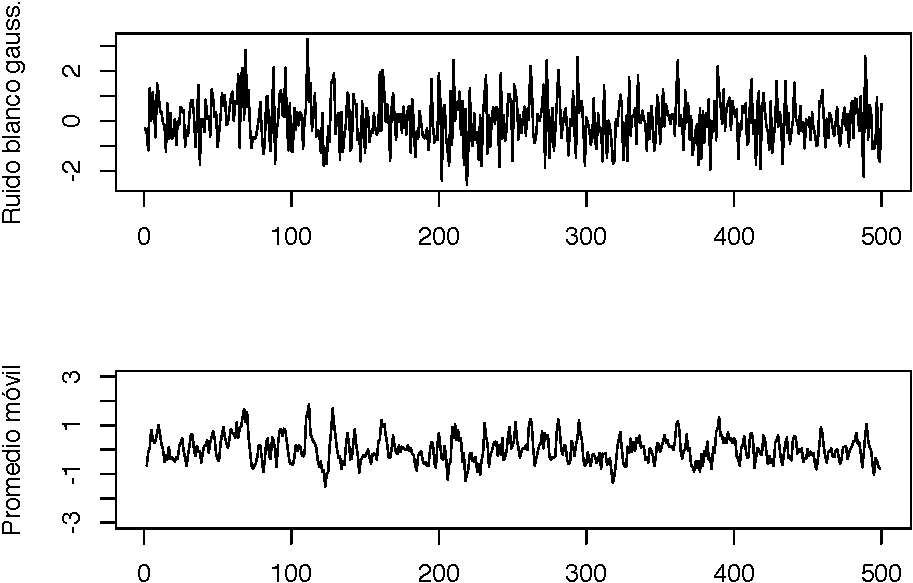
\includegraphics{Serie-de-Tiempo-en-R_files/figure-latex/unnamed-chunk-37-2.pdf}
En la parte superior de cada uno se observan los ruidos blancos y en la
parte inferior los respectivos promedios móviles. Podemos notar que las
series de promedio móvil suavizan el comportamiento de las series
originales, si tomamos más puntos en el promedio mayor será el
suavizado.

\BeginKnitrBlock{example}[Función de media de un promedio móvil]
\protect\hypertarget{exm:ejem-funcion-media-MA}{}{\label{exm:ejem-funcion-media-MA}
\iffalse (Función de media de un promedio móvil) \fi{} }Si \(w_t\)
denota una serie de ruido blanco, entonces
\(\mu_{wt}=\mathbb{E}(w_t)=0\) para todo \(t\). Luego para el promedio
móvil de 3 puntos se tiene
\[\mu_{wt} = \mathbb{E}(v_t) = \frac{1}{3}\mathbb{E}(w_{t-1}+w_t+w_{t+1}) = \frac{1}{3}(\mathbb{E}(w_{t-1})+\mathbb{E}(w_t)+\mathbb{E}(w_{t+1}))=0.\]
\EndKnitrBlock{example}

\BeginKnitrBlock{example}[Autocovarianza de un promedio móvil]
\protect\hypertarget{exm:ejem-ACF-MA}{}{\label{exm:ejem-ACF-MA}
\iffalse (Autocovarianza de un promedio móvil) \fi{} }Consideremos el
promedio móvil de 3 puntos del ejemplo anterior y calculemos su función
de autocovarianza

\begin{eqnarray*}
\gamma_v(s,t) &=& \mathbb{E}[(v_s-\mu_s)(v_t-\mu_t)] \\
      &=& \mathbb{E}[(v_s-o)(v_t-0)] \\
      &=& \frac{1}{9}\mathbb{E}[(w_{s-1}+w_s+w_{s+1})(w_{t-1}+w_t+w_{t+1})]
\end{eqnarray*}

Consideremos \(s-t=h\), para \(h=0,\pm1,\pm2,\ldots\). Entonces, tenemos
para \(h=0\)

\begin{eqnarray*}
\gamma_v(t,t) &=& \frac{1}{9}\mathbb{E}[(w_{t-1}+w_t+w_{t+1})(w_{t-1}+w_t+w_{t+1})] \\
      &=& \frac{1}{9}[\mathbb{E}(w_{t-1}w_{t-1})+\mathbb{E}(w_tw_t)+\mathbb{E}(w_{t+1}w_{t+1})] \\
      &=& \frac{3}{9}
\end{eqnarray*}

Para \(h=1\), tenemos

\begin{eqnarray*}
\gamma_v(t+1,t) &=& \frac{1}{9}\mathbb{E}[(w_t+w_{t+1}+w_{t+2})(w_{t-1}+w_t+w_{t+1})] \\
      &=& \frac{1}{9}[\mathbb{E}(w_tw_t)+\mathbb{E}(w_{t+1}w_{t+1})] \\
      &=& \frac{2}{9}
\end{eqnarray*}

Usando el hecho de que \(\mathbb{E}(w_tw_s)=0\) si \(s\neq t\). Cálculos
similares nos dan
\(\gamma_v(t-1,t)=2/9, \gamma_v(t+2,t)=\gamma_v(t-2,t)=1/9\) y 0 para
\(h\geq3\). Resumiendo se tiene

\begin{equation}
\gamma_v(s,t) = \begin{cases}
                3/9, &\text{ si }s=t\\
                2/9, &\text{ si }|s-t|=1\\
                1/9, &\text{ si }|s-t|=2\\
                0, &\text{ si }|s-t|\geq3
                \end{cases}
\label{eq:eq-autocovarianza-promedio-movil}
\end{equation}
\EndKnitrBlock{example}

\BeginKnitrBlock{example}[Estacionaridad de un promedio móvil]
\protect\hypertarget{exm:ejem-estacionaridad-MA}{}{\label{exm:ejem-estacionaridad-MA}
\iffalse (Estacionaridad de un promedio móvil) \fi{} }El proceso de
promedio móvil usado en los ejemplos
\ref{exm:ejem-promedio-movil-ruido-blanco} y
\ref{exm:ejem-funcion-media-MA} es estacionario ya que podemos escribir
la función de autocovarianza obtenida en
\eqref{eq:eq-autocovarianza-promedio-movil} como
\[\gamma_v(h) = \begin{cases}
                  3/9, &\text{ si }h=0\\
                  2/9, &\text{ si }h=\pm1\\
                  1/9, &\text{ si }h=\pm2\\
                  0, &\text{ si }|h|\geq3
                  \end{cases}\]
\EndKnitrBlock{example}

\BeginKnitrBlock{example}
\protect\hypertarget{exm:ejem-camino-aleatorio}{}{\label{exm:ejem-camino-aleatorio}
}Un modelo para analizar tendencias es el camino aleatorio con tendencia
dado por

\begin{equation}
X_t = \delta+X_{t-1}+w_t
\label{eq:eq-camino-aleatorio-tendencia}
\end{equation}

para \(t=1,2,\ldots,\) con condición inicial \(X_0=0\), y donde \(w_t\)
es un ruido blanco. La constante \(\delta\) es llamada \emph{tendencia},
y cuando \(\delta=0\), \eqref{eq:eq-camino-aleatorio-tendencia} es llamado
simplemente \emph{camino aleatorio}. El término camino aleatorio viene
del hecho de que cuando \(\delta=0\) el valor de la serie de tiempo en
tiempo \(t\) es el valor de la serie de tiempo al tiempo \(t-1\) más un
movimiento completamente aleatorio determinado por \(w_t\). La expresión
\eqref{eq:eq-camino-aleatorio-tendencia} la podemos reescribir como una
suma de variables de ruido blanco, esto es,

\begin{equation}
X_t = \delta t+\sum_{j=1}^Nw_j
\label{eq:eq-camino-aleatorio-suma}
\end{equation}

para \(t=1,2,\ldots.\) A continuación generaremos un camino aleatorio
usando \textbf{R}
\EndKnitrBlock{example}

\begin{Shaded}
\begin{Highlighting}[]
\KeywordTok{set.seed}\NormalTok{(}\DecValTok{154}\NormalTok{)}
\NormalTok{w=}\KeywordTok{rnorm}\NormalTok{(}\DecValTok{500}\NormalTok{,}\DecValTok{0}\NormalTok{,}\DecValTok{1}\NormalTok{)}
\NormalTok{X=}\KeywordTok{cumsum}\NormalTok{(w)}
\NormalTok{wd=w}\OperatorTok{+}\FloatTok{0.2}\NormalTok{; Xd=}\KeywordTok{cumsum}\NormalTok{(wd)}
\KeywordTok{plot.ts}\NormalTok{(Xd,}\DataTypeTok{ylim=}\KeywordTok{c}\NormalTok{(}\OperatorTok{-}\DecValTok{40}\NormalTok{,}\DecValTok{80}\NormalTok{))}
\KeywordTok{lines}\NormalTok{(X,}\DataTypeTok{col=}\StringTok{"red"}\NormalTok{)}
\KeywordTok{lines}\NormalTok{(}\FloatTok{0.2}\OperatorTok{*}\NormalTok{(}\DecValTok{1}\OperatorTok{:}\DecValTok{500}\NormalTok{),}\DataTypeTok{lty=}\StringTok{"dashed"}\NormalTok{,}\DataTypeTok{col=}\StringTok{"blue"}\NormalTok{)}
\end{Highlighting}
\end{Shaded}

\begin{figure}

{\centering 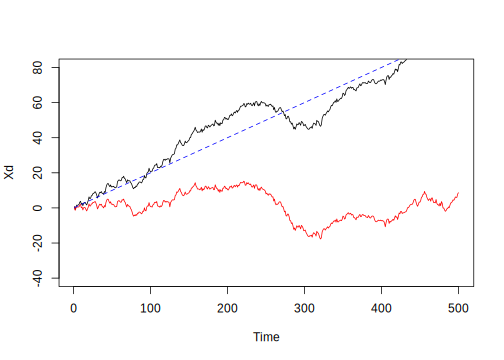
\includegraphics{Serie-de-Tiempo-en-R_files/figure-latex/unnamed-chunk-38-1} 

}

\caption{Gráficos de caminos aleatorios: con tendencia (negro), sin tendencia (rojo)}\label{fig:unnamed-chunk-38}
\end{figure}

\chapter{Modelos AR}\label{modelos-ar}

Los modelos autoregresivos están basados en la idea de que el valor
actual de la serie \(x_t\) se puede explicar como una función de \(p\)
valores pasados \(x_{t-1},x_{t-2},\ldots,x_{t-p}\) donde \(p\) determina
el número de pasos en necesarios para predecir el valor actual. Una
parte de las series de tiempo económicas y financieras suelen ser
caracterizadas por los modelos autorregresivos. Entre los principales
ejemplos de las finanzas tenemos valoración de precios y de dividendos,
las tasas reales de cambio, tasas de interés y los diferenciales de
tipos de interés (spreads).

\BeginKnitrBlock{definition}
\protect\hypertarget{def:defi-modelo-ARp}{}{\label{def:defi-modelo-ARp} }Un
\emph{modelo autoregresivo de orden \(p\)}, abreviado \(AR(p)\) es de la
forma

\begin{equation}
x_t=\phi_1x_{t-1}+\phi_2x_{t-2}+\cdots+\phi_px_{t-p}+w_t,
\label{eq:eq-ARp}
\end{equation}

donde \(x_t\) es estacionario, \(\phi_1\phi_2,\ldots,\phi_p\) son
constantes (\(\phi_p\neq0\)). A menos que se declare lo contrario, se
asume que \(w_t\) es un ruido blanco gaussiano de media cero y varianza
\(\sigma_w^2\). La media de \(x_t\) en \eqref{eq:eq-ARp} es cero. Si la
media \(\mu\) de \(x_t\) no es cero, reemplazamos \(x_t\) por
\(x_t-\mu\) en \eqref{eq:eq-ARp}, es decir

\[x_t-\mu=\phi_1(x_{t-1}-\mu)+\phi_2(x_{t-2}-\mu)+\cdots+\phi_p(x_{t-p}-\mu)+w_t\]

o escribimos

\begin{equation}
x_t=\alpha+\phi_1x_{t-1}+\phi_2x_{t-2}+\cdots+\phi_px_{t-p}+w_t,
\label{eq:eq-ARp-mu}
\end{equation}

donde \(\alpha=\mu(1-\phi_1-\phi_2-\cdots-\phi_p)\).
\EndKnitrBlock{definition}

\begin{center}\rule{0.5\linewidth}{\linethickness}\end{center}

Note que \eqref{eq:eq-ARp-mu} es similar al modelo de regresión dado en
\eqref{eq:eq-regresion-lineal} y por consiguiente el término
\emph{autoregresión}. Sin embargo, se presentan algunas dificultades
técnicas para la aplicación de este modelo, porque los regresores
\(x_{t-1},x_{t-2},\ldots,x_{t-p}\) son aleatorios, mientras que \(x_t\)
se asume fijo. Una forma más útil se deriva de usar el siguiente
operador de cambio dado por \eqref{eq:eq-backward-shift-operator}. Para
escribir el modelo \(AR(p)\) como

\begin{equation}
(1-\phi_1B-\phi_2B^2-\cdots-\phi_pB^p)x_t=w_t
\label{eq:eqARp-operador-B}
\end{equation}

o más conciso como

\begin{equation}
\phi(B)x_t=w_t.
\label{eq:eq-ARp-B-conciso}
\end{equation}

Las propiedades de \(\phi(B)\) son importantes para resolver
\eqref{eq:eq-ARp-B-conciso}. Esto nos lleva a la siguiente definición.

\BeginKnitrBlock{definition}
\protect\hypertarget{def:defi-operador-autoregresivo}{}{\label{def:defi-operador-autoregresivo}
}El \emph{operador autoregresivo} de orden \(p\) se define como

\begin{equation}
\phi(B) = 1-\phi_1B-\phi_2B^2-\cdots-\phi_pB^p
\label{eq:eq-operador-Bp}
\end{equation}
\EndKnitrBlock{definition}

\begin{center}\rule{0.5\linewidth}{\linethickness}\end{center}

\section{Modelo AR(1)}\label{modelo-ar1}

Iniciaremos el estudio de los modelos \(AR\) considerando el modelo de
primer orden \(AR(1)\), dado por \(x_t=\phi x_{t-1}+w_t\). Iterando el
operador de cambio \(k\) veces, obtenemos

\begin{eqnarray*}
x_t &=& \phi x_{t-1}+w_t = \phi(\phi x_{t-2}+w_{t-1})+w_t \\
    &=& \phi^2x_{t-2}+\phi w_{t-1}+w_t \\
    &\vdots& \\
    &=& \phi^kx_{t-k}+\sum_{j=0}^{k-1}\phi^jw_{t-j}.
\end{eqnarray*}

Este método sugiere que por iteración continua del operador de cambio,
siempre que \(|\phi|<1\) y \(x_t\) sea estacionario, podemos representar
un modelo \(AR(1)\) como un proceso lineal dado por \footnote{Note que
  \(\lim_{k\to\infty}\mathbb{E}(x_t-\sum_{j=0}^{\infty}\phi^jw_{t-j})^2 = \lim_{k\to\infty}\phi^{2k}\mathbb{E}(x_{t-k}^2)=0\),
  de modo que \eqref{eq:eq-AR1-serie-lineal} existe en el sentido de media
  cuadrado.}

\begin{equation}
x_t \sum_{j=0}^{\infty}\phi^jw_{t-j}
\label{eq:eq-AR1-serie-lineal}
\end{equation}

El proceso \(AR(1)\) definido en \eqref{eq:eq-AR1-serie-lineal} es
estacionario con media

\[\mathbb{E}(x_t) = \sum_{j=0}^{\infty}\phi^j\mathbb{E}(w_{t-j})=0,\]

y la función de autocovarianza es

\begin{eqnarray}
\gamma(h) &=& Cov(x_{t+h},x_t) \nonumber \\
    &=& \mathbb{E}\left[\left(\sum_{j=0}^{\infty}\phi^jw_{t+h-j}\right) \left(\sum_{k=0}^{\infty}\phi^kw_{t-k}\right)\right] \nonumber \\
    &=& \sigma_w^2\sum_{j=0}^{\infty}\phi^j\phi^{j+h} = \sigma_w^2\phi^h\sum_{j=0}^{\infty}\phi^{2j} \nonumber \\
    &=& \frac{\sigma_w^2\phi^h}{1-\phi^2}, h>0
\label{eq:eq-ACV-AR1}
\end{eqnarray}

Recuerde que \(\gamma(h)=\gamma(-h)\) de modo que basta presentar la
función de autocovarianza para \(h\geq0\).

Si en \eqref{eq:eq-ACV-AR1}, hacemos \(h=0\), obtenemos la varianza del
proceso \(AR(1)\), siendo esta

\[Var(x_t)=\frac{\sigma_w^2}{1-\phi^2},\]

asumiendo que \(\phi_1^2<1\). El requisito de que \(\phi_1^2<1\) resulta
del hecho de que la varianza de una variable aleatoria es acotada y no
negativa. Por consiguiente, la estacionaridad de un modelo \(AR(1)\)
implica que \(-1<\phi_1<1\). Pero si \(-1<\phi_1<1\), entonces por
\eqref{eq:eq-AR1-serie-lineal} y la independencia de \(\{w_t\}\) se puede
demostrar que la media y la varianza de \(x_t\) son finitas. Además, por
la desigualdad de Cauchy-Schwartz todas las autocovarianzas de \(x_t\)
son finitas. Por lo tanto, el modelo \(AR(1)\) es estacionario. En
resumen, una condición necesaria y suficiente para que un proceos
\(AR(1)\) sea estacionario es \(|\phi_1|<1\).

De \eqref{eq:eq-ACV-AR1} la ACF de un modelo \(AR(1)\) es

\begin{equation}
\rho(h) = \frac{\gamma(h)}{\gamma(0)} = \phi^h, \quad h>0
\label{eq:eq-ACF-AR1}
\end{equation}

y \(\rho(h)\) satisface la recursión

\begin{equation}
\rho(h) = \phi\rho(h-1)\text{, para }h=1,2,\ldots.
\label{eq:eq-ACF-AR1-recursiva}
\end{equation}

Las ecuaciones \eqref{eq:eq-ACF-AR1} y \eqref{eq:eq-ACF-AR1-recursiva}
indican que la ACF de un modelo \(AR(1)\) estacionario tiene un
decaimiento exponencial con tasa igual a \(\phi_1\). Si \(\phi_1>0\) el
decaimiento es constante. Si por el contrario, \(\phi_1<0\) entonces el
decaimiento es compuesto y se presenta de forma alternante con tasa
\(\phi_1^2\). Para tener una idea de esto, consideremos los modelos
autoregresivos de orden 1 simulados, para distintos valores de
\(\phi_1\).

\begin{Shaded}
\begin{Highlighting}[]
\CommentTok{# Coeficientes phi}
\NormalTok{phi1=}\FloatTok{0.9}
\NormalTok{phi2=}\OperatorTok{-}\FloatTok{0.8}
\NormalTok{phi3=}\FloatTok{0.4}
\NormalTok{phi4=}\OperatorTok{-}\FloatTok{0.5}
\CommentTok{# Ruido blanco gaussiano}
\NormalTok{w=}\KeywordTok{rnorm}\NormalTok{(}\DecValTok{100}\NormalTok{,}\DecValTok{0}\NormalTok{,}\DecValTok{1}\NormalTok{)}
\CommentTok{# Series AR(1)}
\NormalTok{ar1_}\DecValTok{1}\NormalTok{=}\KeywordTok{filter}\NormalTok{(w,}\DataTypeTok{filter =}\NormalTok{ phi1,}\DataTypeTok{method =} \StringTok{"recursive"}\NormalTok{)}
\NormalTok{ar1_}\DecValTok{2}\NormalTok{=}\KeywordTok{filter}\NormalTok{(w,}\DataTypeTok{filter =}\NormalTok{ phi2,}\DataTypeTok{method =} \StringTok{"recursive"}\NormalTok{)}
\NormalTok{ar1_}\DecValTok{3}\NormalTok{=}\KeywordTok{filter}\NormalTok{(w,}\DataTypeTok{filter =}\NormalTok{ phi3,}\DataTypeTok{method =} \StringTok{"recursive"}\NormalTok{)}
\NormalTok{ar1_}\DecValTok{4}\NormalTok{=}\KeywordTok{filter}\NormalTok{(w,}\DataTypeTok{filter =}\NormalTok{ phi4,}\DataTypeTok{method =} \StringTok{"recursive"}\NormalTok{)}
\CommentTok{# Graficos}
\KeywordTok{par}\NormalTok{(}\DataTypeTok{mfrow=}\KeywordTok{c}\NormalTok{(}\DecValTok{2}\NormalTok{,}\DecValTok{2}\NormalTok{))}
\KeywordTok{plot.ts}\NormalTok{(ar1_}\DecValTok{1}\NormalTok{, }\DataTypeTok{col=}\StringTok{"blue"}\NormalTok{,}\DataTypeTok{type =} \StringTok{"l"}\NormalTok{,}
     \DataTypeTok{main =} \StringTok{"AR(1) con phi=0.9"}\NormalTok{,}\DataTypeTok{xlab=}\StringTok{"t"}\NormalTok{,}\DataTypeTok{ylab=}\StringTok{"x_t"}\NormalTok{)}
\KeywordTok{plot.ts}\NormalTok{(ar1_}\DecValTok{2}\NormalTok{, }\DataTypeTok{col=}\StringTok{"blue"}\NormalTok{,}\DataTypeTok{type =} \StringTok{"l"}\NormalTok{,}
        \DataTypeTok{main =} \StringTok{"AR(1) con phi=-0.8"}\NormalTok{,}\DataTypeTok{xlab=}\StringTok{"t"}\NormalTok{,}\DataTypeTok{ylab=}\StringTok{"x_t"}\NormalTok{)}
\KeywordTok{plot.ts}\NormalTok{(ar1_}\DecValTok{3}\NormalTok{, }\DataTypeTok{col=}\StringTok{"blue"}\NormalTok{,}\DataTypeTok{type =} \StringTok{"l"}\NormalTok{,}
        \DataTypeTok{main =} \StringTok{"AR(1) con phi=0.4"}\NormalTok{,}\DataTypeTok{xlab=}\StringTok{"t"}\NormalTok{,}\DataTypeTok{ylab=}\StringTok{"x_t"}\NormalTok{)}
\KeywordTok{plot.ts}\NormalTok{(ar1_}\DecValTok{4}\NormalTok{, }\DataTypeTok{col=}\StringTok{"blue"}\NormalTok{,}\DataTypeTok{type =} \StringTok{"l"}\NormalTok{,}
        \DataTypeTok{main =} \StringTok{"AR(1) con phi=-0.5"}\NormalTok{,}\DataTypeTok{xlab=}\StringTok{"t"}\NormalTok{,}\DataTypeTok{ylab=}\StringTok{"x_t"}\NormalTok{)}
\end{Highlighting}
\end{Shaded}

\begin{figure}

{\centering 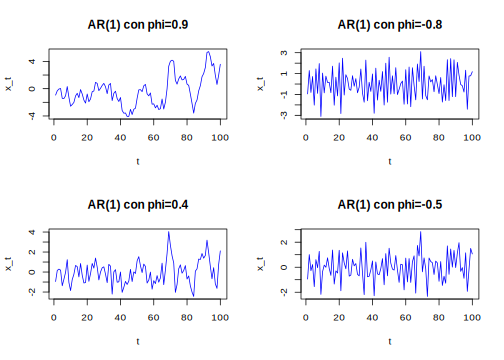
\includegraphics{Serie-de-Tiempo-en-R_files/figure-latex/unnamed-chunk-39-1} 

}

\caption{Simulaciones de procesos autoregresivos de orden 1, AR(1), para distintos valores de $phi_1$}\label{fig:unnamed-chunk-39}
\end{figure}

A continuación mostramos las funciones de autocovarianzas de las series
AR(1) simuladas anteriormente

\begin{Shaded}
\begin{Highlighting}[]
\KeywordTok{par}\NormalTok{(}\DataTypeTok{mfrow=}\KeywordTok{c}\NormalTok{(}\DecValTok{2}\NormalTok{,}\DecValTok{2}\NormalTok{))}
\KeywordTok{acf}\NormalTok{(ar1_}\DecValTok{1}\NormalTok{,}\DataTypeTok{type =} \StringTok{"covariance"}\NormalTok{, }\DataTypeTok{main=}\StringTok{"ACF de la Serie AR(1) con phi=0.9"}\NormalTok{)}
\KeywordTok{acf}\NormalTok{(ar1_}\DecValTok{2}\NormalTok{,}\DataTypeTok{type =} \StringTok{"covariance"}\NormalTok{, }\DataTypeTok{main=}\StringTok{"ACF de la Serie AR(1) con phi=-0.8"}\NormalTok{)}
\KeywordTok{acf}\NormalTok{(ar1_}\DecValTok{3}\NormalTok{,}\DataTypeTok{type =} \StringTok{"covariance"}\NormalTok{, }\DataTypeTok{main=}\StringTok{"ACF de la Serie AR(1) con phi=0.4"}\NormalTok{)}
\KeywordTok{acf}\NormalTok{(ar1_}\DecValTok{4}\NormalTok{,}\DataTypeTok{type =} \StringTok{"covariance"}\NormalTok{, }\DataTypeTok{main=}\StringTok{"ACF de la Serie AR(1) con phi=-0.5"}\NormalTok{)}
\end{Highlighting}
\end{Shaded}

\begin{figure}

{\centering 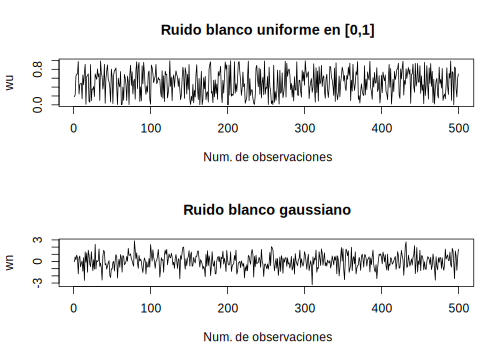
\includegraphics{Serie-de-Tiempo-en-R_files/figure-latex/unnamed-chunk-40-1} 

}

\caption{Funciones de autocovarianzas para las series AR(1) simuladas}\label{fig:unnamed-chunk-40}
\end{figure}

\section{Modelo AR(2)}\label{modelo-ar2}

Un proceso \(AR(2)\) tiene la forma general

\begin{equation}
x_t = \alpha + \phi_1 x_{t-1} + \phi_2 x_{t-2} + w_t
\label{eq:eq-AR2}
\end{equation}

siendo \(\alpha = \mu(1-\phi_1-\phi_2)\), con \(\phi_2\neq 0\). Podemos
calcular su función de media

\begin{eqnarray*}
\mathbb{E}(x_t) &=& \mathbb{E}(\alpha + \phi_1 x_{t-1} + \phi_2 x_{t-2} + w_t) \\
    &=& \alpha+\phi_1\mathbb{E}(x_{t-1})+\phi_2\mathbb{E}(x_{t-2})
\end{eqnarray*}

Por estacionalidad, se tiene que
\(\mathbb{E}(x_t)=\mathbb{E}(x_{t-1})=\mathbb{E}(x_{t-2})\), luego

\[\mathbb{E}(x_t)(1-\phi_1-\phi_2) = \alpha\] Así,
\(\mathbb{E}(x_t) = \frac{\alpha}{1-\phi_1-\phi_2}\), siempre que
\(\phi_1+\phi_2\neq1\). Usando \(\alpha=(1-\phi_1-\phi_2)\mu\) podemos
reescribir el proceso \(AR(2)\) como

\[x_t-\mu = \phi_1(x_{t-1}-\mu)+\phi_2(x_{t-2}-\mu)+w_t.\]

Multiplicando por \(x_{t-h}-\mu\), tenemos

\[(x_{t-h}-\mu)(x_t-\mu) = \phi_1(x_{t-h}-\mu)(x_{t-1}-\mu) + \phi_2(x_{t-h}-\mu)(x_{t-2}-\mu) + (x_{t-h}-\mu)w_t.\]

Tomando valor esperado y usando el hecho de que
\(\mathbb{E}[(x_{t-h}-\mu)w_t]=0\), para \(h>0\), obtenemos

\begin{equation}
\gamma(h) = \phi_1\gamma(h-1)+\phi_2\gamma(h-2) \text{, para }h>0.
\label{eq:eq-ecuacion-momento-AR2}
\end{equation}

Este último resultado se conoce como la \textbf{ecuación de momentos} de
un proceso estacionario \(AR(2)\). Dividiendo
\eqref{eq:eq-ecuacion-momento-AR2} por \(\gamma(0)\), tenemos la propiedad

\begin{equation}
\rho(h) = \phi_1\rho(h-1)+\phi_2\rho(h-2)\text{, para }h>0
\label{eq:eq-ACF-AR2-recursiva}
\end{equation}

para la ACF de \(x_t\). En particular, para paso 1 (\(h=1\)) la ACF
satisface

\[\rho(1) = \phi_1\rho(0)+\phi_2\rho(-1) = \phi_1+\phi_2\rho(1)\]

Por lo tanto, para un proceso \(AR(2)\) estacionario \(x_t\), tenemos

\begin{eqnarray*}
\rho(0) &=& 1 \\
\rho(1) &=& \frac{\phi_1}{1-\phi_2} \\
\rho(h) &=& \phi_1\rho(h-1)+\phi_2\rho(h-2),\quad h\geq2
\end{eqnarray*}

El resultado de la ecuación \eqref{eq:eq-ACF-AR2-recursiva} nos dice que
la ACF de un proceso estacionario \(AR(2)\) satisface la ecuación en
diferencias de segundo orden

\begin{equation}
(1-\phi_1B-\phi_2B^2)\rho(h) = 0
\label{eq:eq-diferencia-ACF}
\end{equation}

donde \(B\) es el operador definido en
\eqref{eq:eq-backward-shift-operator}. La ecuación
\eqref{eq:eq-diferencia-ACF} determina las propiedades de la ACF de un
proceso \(AR(2)\) estacionario. También determina el comportamiento de
los pronósticos de \(x_t\). Correspondiendo a la ecuación en diferencias
anterior, existe una ecuación polinómica de segundo orden

\begin{equation}
x^2-\phi_1x-\phi_2=0
\label{eq:eq-polinomio-2do-orden-AR2}
\end{equation}

Las soluciones de esta ecuación son las raíces características de un
proceso \(AR(2)\) y estas son

\[x=\frac{\phi_1\pm\sqrt{\phi_1^2+4\phi_2}}{2}\]

Denotamos las dos raíces por \(r_1\) y \(r_2\). Si ambos son reales,
entonces la ecuación en diferencias de segundo orden la podemos
factorizar como

\[(1-r_1B)(1-r_2B)\]

y el proceso \(AR(2)\) lo podemos considerar como un proceso \(AR(1)\)
operando sobre otro proceso \(AR(1)\).

La ACF de \(x_t\) es entonces una mezcla de dos decaimientos
exponenciales. Pero si \(\phi_1^2+4\phi_2<0\), entonces \(r_1\) y
\(r_2\) son raíces complejas conjugadas, y el gráfico de la ACF de
\(x_t\) mostrará un amortiguamiento de senos y cosenos.

En aplicaciones financieras y económicas, las raíces caracteríticas
complejas son importantes. Dan lugar al comportamiento de los ciclos
económicos. Por lo tanto, es común que los modelos económicos de series
de tiempo tengan raíces características de valor complejo. Para un
proceso \(AR(2)\) dado por \eqref{eq:eq-AR2} con raíces características
complejas, la longitud \emph{promedio} de un ciclo estocástico es

\[k=\frac{360°}{\arccos(\phi_1/2\sqrt{-\phi_2})},\]

donde el arcocoseno está expresado en grados.

La figura siguiente muestra la ACF de 4 procesos estacionarios
\(AR(2)\). Los procesos \(AR(2)\) mostrados son:

\begin{enumerate}
\def\labelenumi{\alph{enumi})}
\item
  \(x_t=1.2x_{t-1}-0.35x_{t-2}+w_t\)
\item
  \(x_t=0.6x_{t-1}-0.4x_{t-2}+w_t\)
\item
  \(x_t=0.2x_{t-1}+0.35x_{t-2}+w_t\)
\item
  \(x_t=-0.2x_{t-1}+0.35x_{t-2}+w_t\)
\end{enumerate}

\begin{figure}

{\centering 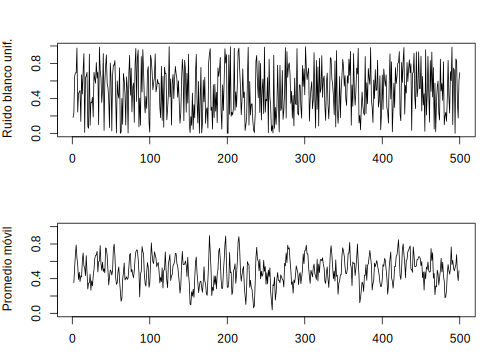
\includegraphics{Serie-de-Tiempo-en-R_files/figure-latex/unnamed-chunk-41-1} 

}

\caption{Cuatro procesos estacionarios AR(2) con distintos valores de phi1 y phi2}\label{fig:unnamed-chunk-41}
\end{figure}

\begin{figure}

{\centering 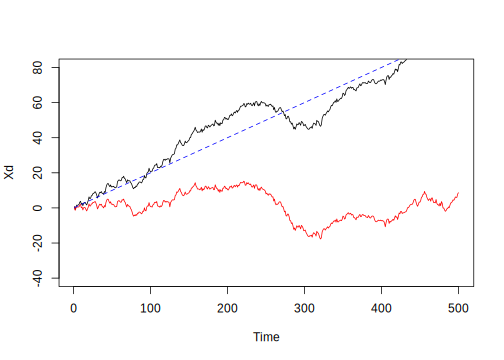
\includegraphics{Serie-de-Tiempo-en-R_files/figure-latex/unnamed-chunk-42-1} 

}

\caption{ACF de 4 procesos estacionarios AR(2) con distintos valores de phi1 y phi2}\label{fig:unnamed-chunk-42}
\end{figure}

La serie (b) tiene raíces características complejas, en efecto

\[\phi_1^2+4\phi_2=(0.6)^2+4\times(-0.4)-1.24<0\]

Se puede notar que n el gráfico de la ACF que este exhibe un
comportamiento de ondas de senos y cosenos. Los otros 3 procesos
\(AR(2)\) tienen raíces características reales, por lo que las ACF
decaen exponencialmente. La condición de estacionaridad de un proceso
\(AR(2)\) es que los valores absolutos de sus raíces características
sean menor que uno, esto es \(|\phi_1|<1, |\phi_2|<1\). Bajo esta
condición, la ecuación recursiva \eqref{eq:eq-ACF-AR2-recursiva} asegura
que la ACF del proceso converge a cero cuando el salto \(h\) crece. Esta
propiedad de convergencia es una condición necesaria para una serie de
tiempo estacionaria. De hecho, la condición también aplica para un
proceso \(AR(1)\) donde la ecuación polinómica es \(x-\phi_1=0\). La
raíz característica es \(x=\phi_1\), la cual debe ser menor que uno en
módulo para que \(x_t\) sea estacionario. Como mostramos antes, para un
proceso estacionario \(AR(1)\) la ACF es \(\rho(h)=\phi^h\),
\eqref{eq:eq-ACF-AR1}.

Así, la condición \(|\phi|<1\), asegura que \(\rho(h)=\phi^h\to0\),
cuando \(h\to\infty\).

\section{Procesos AR(p)}\label{procesos-arp}

Los resultados de los procesos \(AR(1)\) y \(AR(2)\), los podemos
generalizar a procesos \(AR(p)\). Así, la función de media del proceso
\(AR(p)\) estacionario será

\begin{equation}
\mathbb{E}(x_t) = \frac{\alpha}{1-\phi_1-\cdots-\phi_p}
\label{eq:eq-funcion-media-ARp}
\end{equation}

siempre que el denominador sea distinto de cero. La ecuación polinómica
asociada al modelo es

\begin{equation}
x^p-\phi_1x^{p-1}-\phi_2x^{p-2}-\cdots-\phi_p=0
\label{eq:eq-polinomio-ARp}
\end{equation}

la cual nos referimos como la \emph{ecuación característica} del modelo.
Si todas las \emph{raíces caractarísticas} de esta ecuación son menores
qye uno en módulo, esto es \(|r_j|<1\), con \(j=1,\ldots,p\), entonces
la serie \(x_t\) es estacionaria. Para un proceso \(AR(p)\)
estacionario, la ACF satisface la ecuación en diferencias

\[(1-\phi_1B-\phi_2B^2-\cdots-\phi_pB^p)\rho(h)=0\text{, para }h>0.\]

El gráfico de la ACF de un proceso \(AR(p)\) estacionario mostrará una
mezcla de ondas de senos y cosenos con decaimientos exponenciales
dependiendo de la naturaleza de sus raíces características.

\BeginKnitrBlock{example}
\protect\hypertarget{exm:unnamed-chunk-43}{}{\label{exm:unnamed-chunk-43}
}Consideremos el modelo \(AR(3)\) de la forma

\[x_t=0.0047+0.35x_{t-1}+0.18x_{t-2}-0.14x_{t-3}+w_t.\]

Reescribiendo el proceso como

\[x_t-0.35x_{t-1}-0.18x_{t-2}+0.14x_{t-3}=0.0047+w_t\]

obtenemos la correspondiente ecuación en diferencias de orden 3,

\[(1-0.35B-0.18B^2+0.14B^3)=0\]

la cual podemos factorizar como

\[(1+0.52B)(1-0.87B+0.27B^2)=0\]

El primer factor \((1+0.52B)=0\), muestra u ndecaimiento exponencial en
la ACF. Veamos ahora el segundo factor \((1-0.87B-(-0.27)B^2)=0\),
tenemos que \(\phi_1^2+4\phi_2=(0.87)^2+4(-0.27)=-0.3231<0\). Por
consiguiente la ACF mostrará un comportamiento en ondas de senos y
cosenos.
\EndKnitrBlock{example}

\begin{Shaded}
\begin{Highlighting}[]
\NormalTok{xt<-}\KeywordTok{arima.sim}\NormalTok{(}\KeywordTok{list}\NormalTok{(}\DataTypeTok{order=}\KeywordTok{c}\NormalTok{(}\DecValTok{3}\NormalTok{,}\DecValTok{0}\NormalTok{,}\DecValTok{0}\NormalTok{),}\DataTypeTok{ar=}\KeywordTok{c}\NormalTok{(}\FloatTok{0.35}\NormalTok{,}\FloatTok{0.18}\NormalTok{,}\OperatorTok{-}\FloatTok{0.14}\NormalTok{)),}\DataTypeTok{n=}\DecValTok{100}\NormalTok{)}
\KeywordTok{par}\NormalTok{(}\DataTypeTok{mfrow=}\KeywordTok{c}\NormalTok{(}\DecValTok{2}\NormalTok{,}\DecValTok{1}\NormalTok{))}
\KeywordTok{plot}\NormalTok{(xt,}\DataTypeTok{type=}\StringTok{"l"}\NormalTok{,}\DataTypeTok{main=}\StringTok{"Proceso AR(3)"}\NormalTok{)}
\KeywordTok{acf}\NormalTok{(xt, }\DataTypeTok{main=}\StringTok{"ACF para el proceso AR(3)"}\NormalTok{)}
\end{Highlighting}
\end{Shaded}

\begin{center}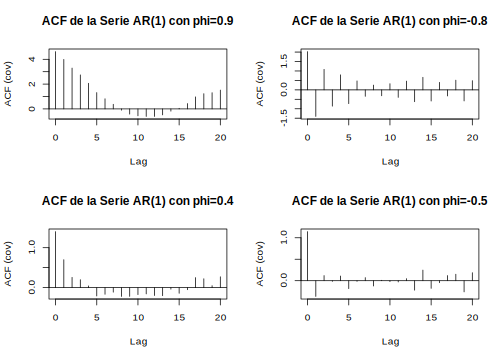
\includegraphics{Serie-de-Tiempo-en-R_files/figure-latex/unnamed-chunk-44-1} \end{center}

\cleardoublepage 

\appendix \addcontentsline{toc}{chapter}{\appendixname}


\bibliography{book.bib,packages.bib}

\backmatter
\printindex

\end{document}
